% Chap05 Derivatives
\section*{Learning Objectives}
By the end of this chapter, the student should be able to:
\begin{itemize}
\item Understand two conceptual views of a single-variable derivative
\item Appreciate the effectiveness of various software tools for computing derivatives
\item See real problems where single-variable derivatives are important in engineering.
\item Make the leap to partial derivatives, which are single-variable derivatives applied to multivariable functions.
\end{itemize}

\section*{Outcomes}
Upon successful completion of this chapter, students will be able to:
\begin{itemize}
 \item Apply the definition of the derivative as rise over run in the limit.
 \item Understand the centrality of the derivative for linear approximation of a function.
 \item Compute a few derivatives via the rise over run definition.
 \item Obtain a sense of when common functions are differentiable and when they are not.
 \item Learn how to compute derivatives with various software packages.
 \item Master the Rules of Differentiation and Understand their Origin.
  \item Apply single-variable derivatives to determine speed from position.
  \item Apply the fact that a strictly positive derivative implies the function is strictly monotonically increasing.
 \item Use L'H\^opital's Rule for limits of indeterminate form.
  \item Compute Jacobians, gradients, and Hessians, with examples using software. 
\item Understand and use the total derivative.
 \end{itemize}


\newpage



\begin{figure}[htb]%
\centering
\subfloat[]{%
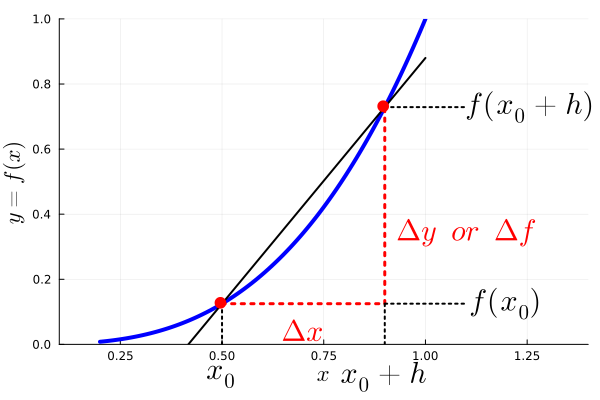
\includegraphics[width=0.45\columnwidth]{graphics/Chap05/DerivativeDefinitionA.png}}%
\hfill
\subfloat[]{%
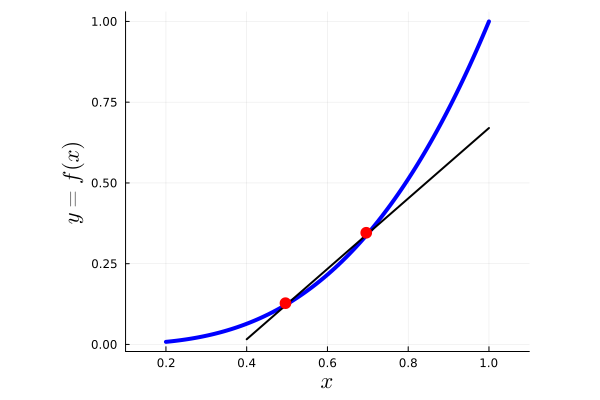
\includegraphics[width=0.45\columnwidth]{graphics/Chap05/DerivativeDefinitionB.png}}%
\hfill
\newline
\subfloat[]{%
	%\centering
 \hspace{-25pt}
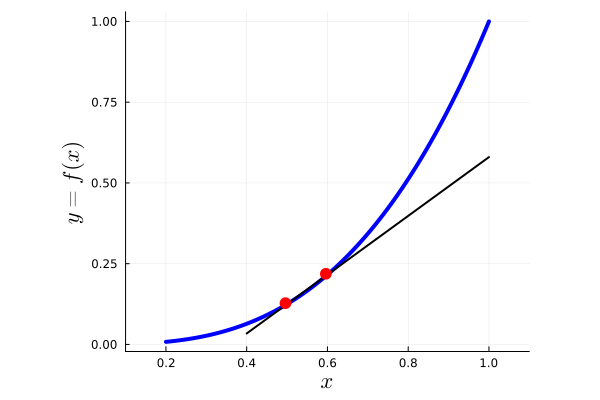
\includegraphics[width=0.45\columnwidth]{graphics/Chap05/DerivativeDefinitionC.png}}%
\hspace{35pt}
\hfill%
\subfloat[]{%
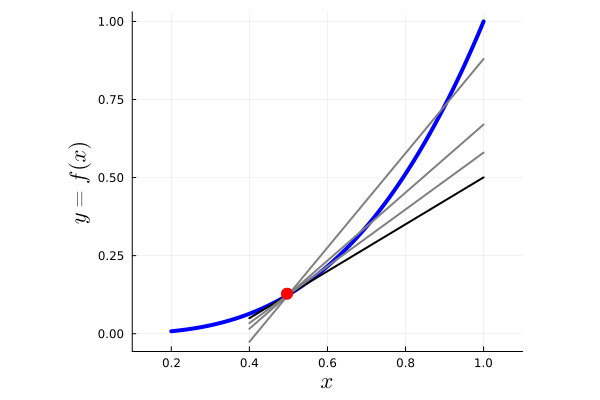
\includegraphics[width=0.45\columnwidth]{graphics/Chap05/DerivativeDefinitionD.png}}%
\hfill
    \caption[]{The derivative of $f:(a, b) \to \real$ at $x_0 \in (a, b)$ is the limiting value of the ``rise over run,'' as $h \to 0$. (a) Graphical definition of all the terms in \eqref{eq:derivAtPoint}. The ``rise'' is $\Delta f := f(x_0+h) - f(x_0)$, and the ``run'' is $\Delta x:= (x_0+h) - x_0 = h$; the slope, of course, is their ratio, $\frac{\Delta f}{\Delta x}$. A line passing through the pair of points $(x_0, f(x_0))$ and $(x_0+h, f(x_0 +h))$ is called a \href{https://en.wikipedia.org/wiki/Secant}{\bf secant line}, where the term ``secant'' is Latin for ``cutting'' (it cuts the function at the two indicated points, as opposed to a ``tangent line'', which touches the function at only one point). (b) and (c) show that as the run, $\Delta x := (x_0 + h) - x_0 = h$, gets smaller and smaller, so does the rise, $\Delta f:= f(x_0 +h) - f(x_0)$. (d) Shows the ``limiting case'' where the secant line becomes a tangent line (indicated by the dark line), the slope of which is the value of the derivative at $x_0$. The lighter lines are the previous secant lines so that we can see the convergence process playing out as $h \to 0$.}
    \label{fig:DefDerivativeAtPoint}
\end{figure}

\section{The Derivative as the Local Slope of a Function}

Figure~\ref{fig:DefDerivativeAtPoint} illustrates the notion of the \textbf{derivative of a function at a point} as the limiting \textbf{slope}, or \textbf{rise over run}, as the run approaches zero (from both sides). 

\begin{tcolorbox}[colback=mylightblue, title = {\bf Derivative at a Point}, breakable]

\begin{definition}
\label{def:derivAtPoint}
The derivative of $f:(a, b) \to \real$ at a point $x_0 \in (a, b)$ is defined as the limiting value of the rise over run, 
 \begin{equation}
\label{eq:derivAtPoint}
    \frac{ df(x_0) }{d x}:= \lim_{h \to 0} \frac{f(x_0 + h) - f(x_0)}{(x_0+h) - x_0} =  \lim_{h \to 0} \frac{f(x_0 + h) - f(x_0)}{h}.
\end{equation}

\bigskip

\textbf{Notes:} Recall that the double-sided limit $\displaystyle \lim_{h \to 0} \frac{f(x_0 + h) - f(x_0)}{h}$ is equivalent to two single-sided limits,
$$\lim_{h \to 0^-} \frac{f(x_0 + h) - f(x_0)}{h} \text{ and } \lim_{h \to 0^+} \frac{f(x_0 + h) - f(x_0)}{h}.$$
Both have to exist, be finite, and equal for the single-sided limit to exist. To show that a function is \textbf{not differentiable at} $x_0$, it is enough to show any one of the following:
\begin{itemize}
    \item The two one-sided limits both exist and are finite, but they have different values.
    \item One of the limits is infinite.
    \item One of the limits does not exist (aka, is undefined).
\end{itemize}

\vspace{.1cm}

If $f:[a, b] \to \real$ is defined on a closed interval, the derivatives at the two endpoints can be defined via single-sided limits, namely
\label{def:derivAtEndPoints}
 \begin{equation}
\label{eq:derivAtBoundaryPoints}
\begin{aligned}
     \frac{ df(a) }{d x} & := \lim_{h \to 0^+} \frac{f(x_0 + h) - f(x_0)}{h} \\
     \frac{ df(b) }{d x} & := \lim_{h \to 0^-} \frac{f(x_0 + h) - f(x_0)}{h}.
\end{aligned}   
\end{equation}
The derivative at points $a < x_0 < b$ is given by \eqref{eq:derivAtPoint}.
\end{definition}
\end{tcolorbox}

\bigskip



\begin{example}
\label{ex:NonDifferentiableFunction}
Explain why the function $f(x):=|x|$ is not differentiable at $x_0=0$. 
\end{example}

\textbf{Solution:} The key is to compute both single-sided limits at the origin. To make this particularly easy, we note that
$$ f(x) := |x| = \begin{cases}
    ~x & x > 0\\
    -x & x < 0 \\
   ~ 0 & x = 0.
\end{cases}$$
Hence, 
\begin{align*}
  \lim_{h \to 0^+} \frac{f(0 + h) - f(0)}{h} & = \lim_{h \to 0^+} \frac{h}{h} = +1 \\
     \lim_{h \to 0^-} \frac{f(0 + h) - f(0)}{h} & = \lim_{h \to 0^-} \frac{-h}{h} = -1.
\end{align*}
Both limits exist and are finite, but they are not equal. Hence, $|x|$ is not differentiable at the origin. You can check that it is differentiable at all other points.

\Qed
\bigskip

\begin{example}
\label{ex:NonDifferentiableFunction02}
Is the function  $$ f(x) :=  \begin{cases}
    1 + x & x > 0\\
    x & x \le 0.
\end{cases}$$
differentiable at $x_0=0$? 
\end{example}

\textbf{Solution:} \Ans No. The key, once again, is to compute a single-sided limit at the origin. If any one of them does not exist or is unbounded, then the derivative is undefined at that point. 
$$
  \lim_{h \to 0^+} \frac{f(0 + h) - f(0)}{h} = \lim_{h \to 0^+} \frac{1+h}{h} = \infty.
$$
This shows that $f$ is not differentiable at the origin. For completeness, we compute the other derivative, namely
$$
  \lim_{h \to 0^-} \frac{f(0 + h) - f(0)}{h} = \lim_{h \to 0^+} \frac{h}{h} = 1.
$$
Note that the ``jump'' discontinuity at the origin made the function not differentiable at that point. 
\Qed

\bigskip
The following two Propositions are actually equivalent (aka, they state the same fact). At this point in your math education, it's OK not to recognize this immediately. 
\bigskip

\begin{propColor}{Never Differentiable at a Point of Discontinuity}{CondNotDifferntiable}
Suppose $f:[a, b] \to \real$ is discontinuous at $x_0 \in [a, b]$. Then, $f$ is nondifferentiable\footnote{AKA, not differentiable.} at $x_0$. \\

\textbf{Note:} $x_0$ could be a point of discontinuity that arises from a ``jump'' in the function's value at $x_0$, as in Example~\ref{ex:NonDifferentiableFunction02}, or it could be due to something wilder, such as 
$$f(x):=\begin{cases}
    \sin(1/x) & x \neq 0 \\ 0 & x = 0
\end{cases}$$ not being continuous at $x_0=0$ due to ``infinitely rapid variation'' in the function's values near the origin.
\end{propColor}

\bigskip

\begin{propColor}{Differentiable Implies Continuous}{DifferntiableImpliesContinuous}
Suppose $f:[a, b] \to \real$ is differentiable at $x_0 \in [a, b]$. Then, $f$ is continuous at $x_0$.    
\end{propColor}
\bigskip

Why are they equivalent? Well, it's the classic rule in Logic: $(A \implies B) \iff (\lnot B \implies \lnot A)$. In our case, let's select $A$ to be ``$f$ is differentiable at $x_0$'' and $B$ to be ``$f$ is continuous at $x_0$''. Then $(A \implies B)$ is Prop.~\ref{thm:DifferntiableImpliesContinuous}. Continuing, $\lnot B$ is ``$f$ is discontinuous at $x_0$'' and $\lnot A$ is ``$f$ is nondifferentiable at $x_0$''. The content of Prop.~\ref{thm:CondNotDifferntiable} is $(\lnot B \implies \lnot A)$. \\


\emstat{Importantly, the two propositions are NOT telling us that a function is differentiable if, and only if, it is continuous. We've already seen that $|x|$ is not differentiable at the origin even though it is continuous everywhere.}

\bigskip


\begin{example}
\label{ex:CommonDerivativesUsingDefinition}
Compute the derivatives of the functions below at an arbitrary point $x \in \real$. 
\begin{enumerate}
\renewcommand{\labelenumi}{(\alph{enumi})}
\setlength{\itemsep}{.2cm}
    \item $f:\real \to \real$ by $f(x)= x^2$.
    \item $g:\real \to \real$ by $g(x) = e^{x}$.
    \item $k:\real \to \real$ by $k(x) = \sin(x)$.
    \item $\ell:(0, \infty) \to \real$ by $\ell(x) = \ln(x)$.
\end{enumerate}

\end{example}

\textbf{Solutions:} 


\begin{enumerate}
\renewcommand{\labelenumi}{(\alph{enumi})}
\setlength{\itemsep}{.2cm}
    \item $f(x)= x^2$. \Ans $\frac{ df(x) }{d x} = 2x$. You can also write the answer so that $\frac{d}{dx}$ looks like an operation being performed on the function: $\frac{ d }{d x}\left(x^2\right) = 2x$. The operation is one of taking the derivative (when it exists).\\
    
In this problem, as requested, we let the arbitrary point be $x$ instead of $x_0$. This will help us to understand that the derivative of a function is often another function.
\begin{align*}
    \frac{ df(x) }{d x} &= \lim_{h \to 0}  \frac{ f(x+h) - f(x)}{h}  ~~(\text{apply definition})\\
    &= \lim_{h \to 0}  \frac{ (x+h)^2 - x^2}{h}  ~~(\text{plug in the function})\\
    &= \lim_{h \to 0}  \frac{ (x^2 + 2h x + h^2) - x^2}{h}  ~~(\text{expand the square})\\
    &=  \lim_{h \to 0}  \frac{ 2h x + h^2}{h} ~~(\text{algebra})\\
    & = \lim_{h \to 0}  2 x + h ~~(\text{more algebra})\\
    & = 2x.
\end{align*}
    
    
    \item $g(x) = e^{x}$.   \Ans $\frac{ dg(x) }{d x} = e^{x}$.  The solution to this problem uses Example~\ref{ex:KeyExponentialLimit}, which showed that $ \displaystyle \lim_{h \to 0}  \frac{ e^{h} - 1}{h} =1$.

\begin{align*}
    \frac{ dg(x) }{d x} &= \lim_{h \to 0}  \frac{ g(x+h) - g(x)}{h}  ~~(\text{apply definition})\\
    &= \lim_{h \to 0}  \frac{ e^{(x+h)} - e^{x}}{h}  ~~(\text{plug in the function})\\
    &= \lim_{h \to 0}  e^{x} \cdot \frac{ e^{h} - 1}{h}  ~~(\text{factor out}~ e^{x})\\
    &= e^{x} \cdot \lim_{h \to 0}  \frac{ e^{h} - 1}{h}  ~~(\text{move }e^x \text{ outside the limit because it is independent of}~ h)\\
    & = e^x \cdot 1 ~~(\text{Example}~\ref{ex:KeyExponentialLimit}) \\
    & = e^x.
\end{align*}
    
    
    \item $k(x) = \sin(x)$. \Ans $\frac{ dk(x) }{d x} =\cos(x)$. The solution requires two trig identities, namely,
\begin{equation}
\begin{aligned}
    \sin(a+b) &= \cos(a) \cdot \sin(b)  + \sin(a) \cdot \cos(b) \\
    2\sin^2\left(\frac{c}{2}\right) &= 1 - \cos(c).
\end{aligned}    
\end{equation}
and $\displaystyle \lim_{h \to 0}  \frac{ \sin(h) }{h} = 1$ from Example~\ref{ex:SqueezeTheorem}. Related video \href{https://youtu.be/mZiPdyHyUvE}{The Limit (do not use L'H\^opital's Rule)} by \bprp.

    
\begin{align*}
    \frac{ dk(x) }{d x} &= \lim_{h \to 0}  \frac{ k(x+h) - k(x)}{h}  ~~(\text{apply definition})\\
    &= \lim_{h \to 0}  \frac{ \sin(x+h) - \sin(x) }{h}  ~~(\text{plug in the function})\\
    &= \lim_{h \to 0}  \frac{ \left(\cos(x) \cdot \sin(h) + \sin(x) \cdot \cos(h) \right)- \sin(x) }{h}  ~~(\text{use the first identity})\\
    &=  \cos(x) \cdot \lim_{h \to 0}  \frac{ \sin(h) }{h} + \sin(x) \cdot \lim_{h \to 0}  \frac{ \left( \cos(h) -1 \right) }{h} ~~(\text{algebra})\\
    &=  \cos(x) \cdot \lim_{h \to 0}  \frac{ \sin(h) }{h} - \sin(x) \cdot \lim_{h \to 0}  2 \cdot \frac{ \sin^2\left( \frac{h}{2} \right) }{h} ~~(\text{use the second identity})\\
     &=  \cos(x) \cdot 1 -  \sin(x) \cdot \lim_{h \to 0} \sin\left( \frac{h}{2} \right) \cdot \frac{ \sin\left( \frac{h}{2} \right)  }{\frac{h}{2} } ~~(\text{more algebra})\\
     & = \cos(x),
\end{align*}
because from Prop.~\ref{thm:LimitProdRatio}, when we have a product of functions where at least one has a finite limit, then the limit of the product is the product of the limits. Moreover,
$$ \lim_{h \to 0}  \sin\left( \frac{h}{2} \right)=0 \text{ and } \lim_{h \to 0} \frac{ \sin\left(\frac{h}{2}\right)  }{\frac{h}{2}} =1.$$
Therefore, 
\begin{align*}
 \lim_{h \to 0} \left( \sin\left( \frac{h}{2} \right) \right) \cdot \left( \frac{ \sin\left( \frac{h}{2} \right)  }{\frac{h}{2}} \right)&= \underbrace{\left(\lim_{h \to 0}  \sin\left( \frac{h}{2} \right) \right)}_{0} \cdot \underbrace{\left( \lim_{h \to 0} \frac{ \sin\left(\frac{h}{2}\right)  }{\frac{h}{2}} \right) }_{1}~~(\text{Applying Prop.~\ref{thm:LimitProdRatio} and the above limits})\\
     & = 0 \cdot 1 \\
     & = 0.
\end{align*}

 \item $\ell(x) = \ln(x)$. \Ans $\frac{ d\ell(x) }{d x} =\frac{1}{x}$. \\

 We worked this one in Example~\ref{ex:eToPowerxDerivativeNatLogx}-(c).


\end{enumerate} 

\Qed
\vspace*{.2cm}

That's how derivatives are computed via the definition. As a practicing engineer, you will do that like, never in your career, and in your engineering courses, you are unlikely to be asked to compute a derivative by the definition. Hence, we'll not belabor it. Instead, as with continuous functions, we'll close this Section with a list of common functions and their derivatives...once we introduce a second common notation for the derivative of a function.

\vspace*{.2cm}

\begin{tcolorbox}[colback=mylightblue, title = {\bf Notation for Differentiation}, breakable]

\begin{definition}
\label{def:NewtonVsLeibnizNotation}
In Newton's notation for the derivative, the primary objects are functions, such as  $f ( x ) = x^2$, and derivatives are written with a prime, as in $f'( x ) = 2 x$; some claim that Lagrange introduced this notation on the basis of Newton's work. In Leibniz's notation, the primary objects are relationships, such as $y = x^2$, and derivatives are written as a ratio, as in  $\frac{dy}{dx} = 2 x$. Both notations are quite common, and we will even see a third notation (based on dots) when we focus on derivatives with respect to time of a trajectory, such as $x(t)$.
 \begin{equation}
\label{eq:NewtonVsLeibnizNotation}
\begin{aligned}
     f'(x) &: = \lim_{h \to 0} \frac{f(x + h) - f(x)}{h} ~~\textbf{Newton Style}\\
     \frac{df(x)}{dx} &:= \lim_{h \to 0} \frac{f(x + h) - f(x)}{h} ~~\textbf{Leibniz Style}.
\end{aligned}   
\end{equation}

\textbf{Note:} Once again, we could create a perfect bubble in the course where one and only one notation is used, but then you would be at a disadvantage in other courses and life.
\end{definition}
\end{tcolorbox}

\bigskip


\bigskip


% Define a new save box
\newsavebox{\mybox}

% Save the tabular content inside the box
\sbox{\mybox}
{
\renewcommand{\arraystretch}{1.5}
%\begin{tabular}{|l|l|l|}
\begin{tabular}{|>{\bfseries\boldmath}l|>{\bfseries\boldmath}l|>{\bfseries\boldmath}l|}
\hline
Function & Derivative & Domain \\
\hline
$f(x) = c$ & $f'(x) = 0$ & $x \in \real$ \\
$f(x) = x^n$ & $f'(x) = nx^{n-1}$ & $x \in \real$ \\
$f(x) = e^x$ & $f'(x) = e^x$ & $x \in \real$ \\
$f(x) = \ln(x)$ & $f'(x) = \frac{1}{x}$ & $x > 0$ \\
$f(x) = \sin(x)$ & $f'(x) = \cos(x)$ & $x \in \real$ \\
$f(x) = \cos(x)$ & $f'(x) = -\sin(x)$ & $x \in \real$ \\
$f(x) = \tan(x)$ & $f'(x) = \sec^2(x)$ & $x \neq \frac{\pi}{2} + k\pi, \, k \in \whole$ \\
$f(x) = \tan(x)$ & $f'(x) = 1 + \tan^2(x)$ & $x \neq \frac{\pi}{2} + k\pi, \, k \in \whole$ \\
$f(x) = \cot(x)$ & $f'(x) = -\csc^2(x)$ & $x \neq k\pi, \, k \in \whole$ \\
$f(x) = \sec(x)$ & $f'(x) = \sec(x)\tan(x)$ & $x \neq \frac{\pi}{2} + k\pi, \, k \in \whole$ \\
$f(x) = \csc(x)$ & $f'(x) = -\csc(x)\cot(x)$ & $x \neq k\pi, \, k \in \whole$ \\
$f(x) = \sinh(x)$ & $f'(x) = \cosh(x)$ & $x \in \real$ \\
$f(x) = \cosh(x)$ & $f'(x) = \sinh(x)$ & $x \in \real$ \\
$f(x) = \tanh(x)$ & $f'(x) = {\rm sech}^2(x)$ & $x \in \real$ \\
\hline
\end{tabular}
}

\begin{propColor}{Common Functions, Their Derivatives, and Domains}{CommonDiffferentiableFuns}

The following functions are differentiable on the indicated domains. Here, we use Newton's notation for the derivative, namely
$$
    f'(x) : = \lim_{h \to 0} \frac{f(x + h) - f(x)}{h}.
$$

\vspace*{.3cm}
\begin{center}
\usebox{\mybox}
\end{center}
\bigskip

\textbf{Note:} $1 + \tan^2(x)= \left( \frac{\cos(x)}{\cos(x)}\right)^2  + \left( \frac{\sin(x)}{\cos(x)}\right)^2 =  \frac{\sin^2(x) + \cos^2(x)}{\cos^2(x)}   = \left( \frac{1}{\cos(x)}\right)^2  = \sec^2(x) $. Both forms are common for the derivative of $\tan(x)$. In a similar manner, $-\csc^2(x) = -\frac{1}{\sin^2(x)} = - \frac{\sin^2(x) + \cos^2(x)}{\sin^2(x)} = - \left(1 + \cot^2(x)\right)$.

\end{propColor}

\bigskip
\section{The Derivative as a Local Linear Approximation of a Function}
\label{sec:LocalLinearApproxFunction}

Let $f:(a, b) \to \real$ and let $x_0 \in (a, b)$. Suppose we wanted to approximate the function by a line, $y = y_0 + m\cdot (x-x_0)$, near the point $x_0$. Fig.~\ref{fig:DefDerivativeAtPoint} suggests that the derivative is doing something like that. Let's explore it a bit more deeply.\\

We pose
\begin{equation}
    \label{eq:AffineScalarApprox01}
    f(x) \approx  y_0 + m \cdot (x-x_0)
\end{equation}
for $|x-x_0| < \delta$ and some $\delta>0$. What values should we assign to $y_0$ and $m$? Well, if we plug $x =x_0$ into \eqref{eq:AffineScalarApprox01}, we obtain
$$ f(x_0) = y_0.$$
Hence, 
\begin{equation}
    \label{eq:AffineScalarApprox02}
    f(x) \approx  f(x_0) + m( \cdot x-x_0).
\end{equation}
Next, because we are used to limits, we plug in $x=x_0 + h$ into \eqref{eq:AffineScalarApprox02}, yielding
$$ f(x_0 + h) \approx  f(x_0) + \underbrace{m \cdot h}_{h=(x_0 + h)-x_0}.$$
A little algebra gives us
\begin{equation}
    \label{eq:AffineScalarApprox03}
  \big(  f(x_0 + h) - f(x_0) \approx m \cdot h  \big) \iff \left( m \approx  \frac{ f(x_0 + h) - f(x_0) }{h} \right).
\end{equation}
The approximation should be better and better with smaller and smaller $h$. In the limit, we have
\begin{equation}
    \label{eq:AffineScalarApprox04}
m = \lim_{h \to 0} \frac{ f(x_0 + h) - f(x_0) }{h},
\end{equation}
as long as the limit exists. In other symbols, if $f$ is differentiable at $x_0$, then
\begin{equation}
    \label{eq:AffineScalarApprox05}
    f(x) \approx  f(x_0) +  \frac{df(x_0)}{dx} \cdot (x-x_0)
\end{equation}
is a \textbf{local linear approximation} to the function near the point $x_0$.\\

\begin{tcolorbox}[colback=mylightblue, title = {\bf (Optional Read:) More Formal Definition of a Linear Approximation of a Function Near a Point}, breakable]

\begin{definition} Let \(f(x)\) be a differentiable function at \(x_0\). The function \(y(x) = y_0 + m(x - x_0)\) is said to be a \textbf{linear approximation} of \(f(x)\) near \(x_0\) if
\[
\lim_{x \to x_0} \frac{f(x) - \left( y_0 + m(x - x_0) \right)}{x - x_0} = 0.
\]
\end{definition}

Roughly speaking, this definition implies that the error between \( f(x) \) and its linear approximation \( y(x) \)  ``quadratic'' in $x -x_0$.\\

\textbf{Claim:} The only possible values for \( y_0 \) and \( m \) such that \( y(x) = y_0 + m \dot(x - x_0) \) is a linear approximation of \( f(x) \) near \( x_0 \) are \( y_0 = f(x_0) \) and \( m = f'(x_0) \). \\


\textbf{Proof:} Assume that \( y(x) = y_0 + m(x - x_0) \) is a linear approximation of \( f(x) \) near \( x_0 \). By the definition of linear approximation, we have the condition,
\[
\lim_{x \to x_0} \frac{f(x) - \left( y_0 + m(x - x_0) \right)}{x - x_0} = 0.
\]

Expanding the numerator gives,

\[
f(x) - \left( y_0 + m(x - x_0) \right) = f(x) - y_0 - m(x - x_0).
\]
thus, the condition becomes,

\[
\lim_{x \to x_0} \frac{f(x) - y_0 - m(x - x_0)}{x - x_0} = 0.
\]

We can rewrite this as,

\[
\lim_{x \to x_0} \left( \frac{f(x) - f(x_0)}{x - x_0} + \frac{f(x_0) - y_0}{x - x_0} - m \right) = 0.
\]

Using the fact that \( \lim_{x \to x_0} \frac{f(x) - f(x_0)}{x - x_0} = f'(x_0) \), we obtain,

\[
f'(x_0) + \lim_{x \to x_0} \frac{f(x_0) - y_0}{x - x_0} - m = 0.
\]

Now, observe that \( \lim_{x \to x_0} \frac{f(x_0) - y_0}{x - x_0} \) is only well-defined if \( f(x_0) = y_0 \), otherwise the limit would not exist (it would go to infinity). Therefore, we must have,

\[
y_0 = f(x_0).
\]

Substituting this back into the equation, we obtain,
\[
f'(x_0) - m = 0,
\]

which implied,

\[
m = f'(x_0).
\]

Thus, the only possible values for \( y_0 \) and \( m \) are \( y_0 = f(x_0) \) and \( m = f'(x_0) \).

\Qed
\end{tcolorbox}

Later in the Chapter, we will see how derivatives help us to build local quadratic, cubic, ..., $n$-th degree polynomial approximations to functions. These have two names: Maclaurin series when the approximation is performed at the origin (i.e., $x_0 = 0$) and \href{https://en.wikipedia.org/wiki/Taylor_series}{Taylor Series} when $x_0 \neq 0$. 

\bigskip

\begin{factColor}{(Optional Read:) Quality of the Approximation of a Linear Approximation}{QualityLinearApproximationm}
To approximate a function \( f(x) \) at a point \( x \) using its behavior near \( x \), we can expand it in terms of a small increment \( h \). The first-order approximation, often referred to as the linear approximation, assumes that \( f(x+h) \) can be expressed as:

\[
f(x+h) \approx f(x) + f'(x) \cdot h,
\]

which implies that the change in \( f \) is primarily governed by its derivative at \( x \). This approximation is valid for small values of \( h \), where higher-order terms become negligible. 

To rigorously understand the accuracy of this approximation, we consider the error term,
\[
{\rm Error(h)} := f(x+h) - \left(f(x) + f'(x) \cdot h\right).
\]
The first-order approximation assumes that this error is of order \( h^2 \), meaning it diminishes much faster than \( h \) as \( h \to 0 \). Mathematically, we can write:

\[
\lim_{h \to 0} \frac{f(x+h) - f(x) - f'(x) \cdot h}{h^2} = 0.
\]

This statement ensures that the remainder of the approximation is proportional to \( h^2 \) and becomes insignificant for small \( h \). Thus, the first-order approximation provides a simple yet powerful tool to estimate \( f(x+h) \), while the error term analysis assures its accuracy.
\end{factColor}

\emstat{It's not worth doing much more with derivatives until you believe they are very easy to compute with modern software tools. Once you see that you can throw a ``derivative party'' without breaking a sweat, you'll be more inclined to understand how useful derivatives can be.}

% \bigskip
% \bigskip
% \bigskip
% \bigskip

\section{Software Tools for Computing Derivatives}

This section is based on ROB 101 \textit{Computational Linear Algebra}: Lab 10, developed by Dr. Alphonsus Antwi Adu-Bredu when he was a PhD student at the University of Michigan, Department of Robotics. He presents three methods to compute derivatives. Here is a link to the \href{https://www.dropbox.com/s/lc4g6qqbnrb826n/ROB_101_Julia_Programming_Guide_31January2023.pdf?dl=0}{ROB 101 Programming Guide}.

\subsection{Symbolic Derivatives}
\label{sec:SymbolicDerivatives}

Symbolic means computing derivatives and manipulating functions the way a human would on a sheet of paper. You define variables that are ``symbolic'' (aka, do not take on numerical values, such as $x$, $y$, or $z$), and you manipulate them as variables. It's pretty incredible that a machine designed to crunch numbers can do that. \\

\begin{lstlisting}[language=Julia,style=mystyle]
using Symbolics # Only need to do this once per session

# Create a custom function to make differentiation convenient
function deriv(f, x)
    return expand_derivatives(Differential(x)(f))
end

# Sample Usage
@variables x # Makes x a symbolic variable
f = x^3*cos(x) + x^2*sin(x)^2 + log(3x) # Note we did not say f(x) =, just f = 
dfdx = deriv(f, x)
\end{lstlisting}
\textbf{Output} 
$$
\frac{1}{x} - x^{3} \sin\left( x \right) + 2 \sin^{2}\left( x \right) x + 3 x^{2} \cos\left( x \right) + 2 x^{2} \cos\left( x \right) \sin\left( x \right)
$$
Recall that in Julia, $\log(x) = \ln(x)$ and all trig functions are in radians. \\

\vspace*{.2cm}
The above gives us the derivative as a function of x. If we want to evaluate it at a point, say $x_0 = 0.5$, we can do so as follows, with a convenient, custom-made function  
\vspace*{.2cm}
\begin{lstlisting}[language=Julia,style=mystyle]
function evaluate(f, x0)
   return  Symbolics.value(substitute(f, (Dict(x => x0))))
end

# Example use
@show dfdx
evaluate(dfdx, .5)
\end{lstlisting}
\textbf{Output} 
\begin{verbatim}
dfdx = 1 / x + 2x*(sin(x)^2) + 3(x^2)*cos(x) + 2(x^2)*cos(x)*sin(x) - (x^3)*sin(x)

3.0384753223601586
\end{verbatim}
\vspace*{.2cm}
\textbf{Note:} The output of \texttt{substitute(f, (Dict(x => x0)))} has Type \texttt{Num} as you can check with the
command \texttt{typeof}
\begin{lstlisting}[language=Julia,style=mystyle]
val_numeric = substitute(dfdx, (Dict(x => 0.5))) # Will be Type Num

@show typeof(val_numeric)

val = Symbolics.value(val_numeric) # converts to Float64
\end{lstlisting}
\textbf{Output} 
\begin{verbatim}
typeof(val_numeric) = Num

3.0384753223601586
\end{verbatim}
It is recommended that you use\footnote{Yes, you have to write your version of the function!} the ``evaluate'' command created above. It is, for some reason, not a part of the Symbolic.jl package.

\vspace*{.2cm}
Continuing with our demonstration of symbolic differentiation, one can even compute the derivative of the derivative! It goes like so:
\vspace*{.2cm}
\begin{lstlisting}[language=Julia,style=mystyle]
d2fdx2 = deriv(dfdx, x)
\end{lstlisting}
\textbf{Output} 
$$\frac{-1}{x^{2}} + 2 \sin^{2}\left( x \right) + 2 \cos^{2}\left( x \right) x^{2} - x^{3} \cos\left( x \right) + 6 x \cos\left( x \right) - 2 \sin^{2}\left( x \right) x^{2} - 6 x^{2} \sin\left( x \right) + 8 x \cos\left( x \right) \sin\left( x \right)$$
\vspace*{.2cm}
And, we can go completely bonkers and put the derivative operation in a loop, like so
\vspace*{.2cm}
\begin{lstlisting}[language=Julia,style=mystyle]
@variables x
f = x^3*cos(x) + x^2*sin(x)^2 + log(3x)
N=5
temp = f
for k = 1:N
    temp= deriv(temp, x)
end
dNfdxN = temp
\end{lstlisting}
\textbf{Output} 
\begin{align*}
   \frac{-32}{x^{5}} - 60 \cos\left( x \right) - 80 \cos^{2}\left( x \right) x - 4 x^{3} \frac{2}{x^{8}} - x^{3} \sin\left( x \right) + 60 x \sin\left( x \right) \\
   \hspace*{.5cm}
   + 80 \sin^{2}\left( x \right) x - 64 x^{11} \frac{-1}{x^{16}} + 15 x^{2} \cos\left( x \right) \\ - 160 \cos\left( x \right) \sin\left( x \right) + 32 x^{2} 
   \cos\left( x \right) \sin\left( x \right). 
\end{align*}

\vspace*{.2cm}
\textbf{Note that the awkward expression, $$-4 x^{3} \frac{2}{x^{8}} - 64 x^{11} \frac{-1}{x^{16}},$$ was not simplified}. We can fix that as follows,
\vspace*{.2cm}
\begin{lstlisting}[language=Julia,style=mystyle]
# Added a simplify operation
function deriv(f, x)
    df = Differential(x)(f)
    return simplify(expand_derivatives(df)) # Note the simplify command
end

# Example use
@variables x
f = x^3*cos(x) + x^2*sin(x)^2 + log(3x)
N=5
temp = f
for k = 1:N
    temp= deriv(temp, x)
end
dNfdxN = temp
\end{lstlisting}
\textbf{Output} 
\begin{align*}
    \frac{24}{x^{5}} + 6 \left(  - \cos\left( x \right) - 4\sin\left( 2x \right) \right) - 54\cos\left( x \right) - 56\sin\left( 2x \right) - x^{3} \sin\left( x \right) + 15x^{2} \cos\left( x \right) + 60x \sin\left( x \right) + 16x^{2} \sin\left( 2x \right) - 80x \cos\left( 2x \right)
\end{align*}

\textcolor{red}{\bf The ``cost'' is that the function runs slower.} Hence, it's your call: to \texttt{simplify} or not to \texttt{simplify}, that is the question!

\textbf{Advantages of Symbolic Differentiation}
\begin{itemize}
    \item Symbolic Differentiation allows you to compute exact derivatives up to machine precision.
    \item Symbolic Differentiation is also a great tool for analysis. Being able to generate closed-form derivatives of a model facilitates the understanding of the dynamics of the model.
    \item Symbolic Differentiation is also significantly useful for generating closed-form derivatives of functions as code. Closed-loop controllers running on real-time systems often have to run at frequencies in the 1kHz range. This constrains the control loop to a time budget of 1 millisecond. Given this time budget, operations in the controller (such as computing derivatives and Jacobians) have to be as fast as possible. Being able to generate closed-form parameterized functions for derivatives and Jacobians offline using Symbolic differentiation that can then be evaluated online in microseconds can be very useful in speeding up your controller and meeting the controller time budget.
\end{itemize}


\subsection*{Disadvantages of Symbolic Differentiation}
\begin{itemize}
    \item The main disadvantage of symbolic derivatives is that they tend to get gnarly and exponentially long very quickly. This phenomenon is called \textbf{Expression swell}. Imagine taking the derivative of a function 
    $$
    h(x) = f(x)g(x)
    $$ 
    where $f(x)$ is itself the product $f(x) = u(x)v(x)$, the derivative of $h(x)$ ends up as this gnarly function 
    $$
    \frac{d}{dx}h(x) = \left(\frac{d}{dx}u(x)v(x) + u(x)\frac{d}{dx}v(x)\right)g(x) + u(x)v(x)\frac{d}{dx}g(x)
    $$
    leading to inefficient code. We will learn the \textbf{Product Rule} in Chapter~\ref{sec:DiffRules}. 
\end{itemize}

\subsection{Numerical Differentiation}

Numerical Differentiation, also called \textbf{finite differences}, was the primary method we used in ROB 101 \textit{Computational Linear Algebra}. 

\begin{tcolorbox}[title=\textbf{Numerical Approximations of a Derivative}, breakable]

Common approximations of a derivative are based on ``not letting the limit go all the way to zero'' but stopping at $h$ small.
 \begin{equation}
\label{eq:forwardDifferenceV01}
    \frac{ df(x_0) }{d x}:= \lim_{h \to 0} \frac{f(x_0 + h) - f(x_0)}{h}.
\end{equation}
In practice, we will use ``small values'' for $h$ and never compute the exact limit. Hence, we have an \textbf{approximation for the derivative} at a point, namely
\begin{equation}
\label{eq:forwardDifference}
    \frac{df(x_0)}{dx}\approx \frac{f(x_0 + h) - f(x_0)}{h},
\end{equation}
which is called a \textbf{forward difference approximation to the derivative}.\\

We can also do a \textbf{backward difference approximation to the derivative},
\begin{equation}
\label{eq:backwardDifference}
   \frac{df(x_0)}{dx}\approx \frac{f(x_0) - f(x_0-  h)}{h},
\end{equation}
and a \textbf{symmetric difference approximation}, where we go both forward and backward from the point $x_0$,
\begin{equation}
\label{eq:symmetricDifference}
   \frac{df(x_0)}{dx}\approx \frac{f(x_0 + h)- f(x_0-  h)}{2 h}.
\end{equation}
The forward and backward difference approximations to the derivative are, in fact, exact for linear functions, while the symmetric difference approximation is \textit{exact} for quadratic polynomials. The symmetric difference is also sometimes called a \textbf{central difference}.\\

\textbf{If the derivative of $\mathbf{f(x)}$ at a point $\mathbf{x_0}$ exists, then for $\mathbf{h}$ sufficiently small, the forward difference, backward difference, and symmetric difference approximations to the derivative will always agree. If they provide different answers, then the limit in \eqref{eq:forwardDifferenceV01} does not exist, and the function is said to be nondifferentiable.}

\end{tcolorbox}

\bigskip

In Julia, you do numerical derivatives as follows. \\


\begin{lstlisting}[language=Julia,style=mystyle]
using FiniteDiff # Julia package for finite difference approximations of derivatives.

# Example function
g(x) = x^3*cos(x) + x^2*sin(x)^2 + log(3x)

val = FiniteDiff.finite_difference_derivative(g, 0.5)
\end{lstlisting}
\textbf{Output} 
\begin{verbatim}
3.038475322499568
\end{verbatim}

\textcolor{red}{\bf The ``true'' (symbolic) value was $3.0384753223601586$; their difference is $1.394 \times 10^{-10}$.} That seems pretty good! Note that the \texttt{FiniteDiff} package chooses the value of ``$h>0$'' for you, which is pretty sweet. 

\vspace*{.2cm}

\subsection*{Advantages of Numerical Differentiation}
\begin{itemize}
    \item Numerical differentiation is the simplest differentiation method to implement. It only depends on the function values and not on any set of differential calculus rules.
    \item In view of this, numerical differentiation can be applied to any differentiable function to get reasonably accurate results.
\end{itemize}

\subsection*{Disadvantages of Numerical Differentiation}
\begin{itemize}
    \item Finite Difference suffers from \textit{Truncation error} resulting in inaccurate derivatives when the step size is large.
    \item Finite Difference can also be expensive to compute for functions with large input dimensions. This is more important when we get to Jacobians and gradients.
    \item It is not easy to ``iterate'' numerical differentiation methods. We had to develop special formulas for that in ROB 101.
\end{itemize}



\subsection{Automatic Differentiation}
\label{sec:AutomaticDifferentiation}

Similar to Symbolic Differentiation, \textbf{Automatic Differentiation (aka, AD)} uses differential calculus rules to compute derivatives. \textcolor{blue}{\bf However, its goal is to return a numerical solution instead of a single closed-form analytical expression}. As such, Automatic Differentiation keeps track of intermediate variables and their derivatives to speed up computation. It decomposes the function into primitive operations using the ``chain rule'', evaluates the operations and their derivatives, and stores them in intermediate variables. We cover the \textbf{chain rule} in Chapter~\ref{sec:DiffRules}. Your author thinks of Automatic Differentiation as ``the chain rule meets databases''! It is very efficient. 

There are two primary forms of automatic differentiation, \textbf{Forward Mode AD}
\begin{itemize}
    \item In forward mode AD, the derivative information is propagated from the input variables through to the output of the function.
    \item This is done by augmenting each intermediate variable in the computation with its derivative (or tangent) with respect to the input variables.
    \item Forward mode is particularly efficient when the number of input variables is small compared to the number of output variables.
\end{itemize}

There is also \textbf{Reverse Mode AD}
\begin{itemize}
    \item In reverse mode AD, the derivative information is propagated from the output back to the input variables.
    \item This is done by computing the adjoint or cotangent of each intermediate variable, which represents the rate of change of the output with respect to that intermediate variable.
    \item The adjoints are then used to compute the gradient of the output with respect to the input variables.
    \item Reverse mode is particularly efficient when the number of output variables is small compared to the number of input variables. This property makes it especially popular in deep learning, where the objective is typically scalar (e.g., loss) but the input (e.g., parameters of a neural network) is high-dimensional.
\end{itemize}

Both forward and reverse modes of AD are exact methods (up to machine precision) and are more accurate than numerical differentiation, which can suffer from truncation and rounding errors. In addition to these primary forms, there are also hybrid methods that combine aspects of both forward and reverse modes to optimize the computation of derivatives for specific types of functions or computational graphs (e.g., Neural Networks). 

% \begin{center}
% \setlength{\fboxrule}{2pt}  % Setting the thickness of the border line
%    \fbox{ \parbox{0.9\linewidth}{\textcolor{red}{\bf At this point in your Calculus education, keeping all these methods straight is not important.} What you should take away is that differentiation is an operation to extract information from functions. Until recently, differentiation was a painful manual process. Today, you have tons of options for computing derivatives. Modern AI would not exist without these methods; it relies especially on Automatic Differentiation for the training process of Neural Networks. Each tool has its place. {\bf In other science and engineering courses, you may be terrified by the complicated functions you are asked to differentiate because you have to do it by hand, maybe even on an exam. As a practicing engineer, it's cake. Crazy world, huh?}
% }
% } 
% \end{center}

\emstat{\textcolor{blue}{\bf At this point in your Calculus education, keeping all these methods straight is not important.} What you should take away is that differentiation is an operation to extract information from functions. Until recently, differentiation was a painful manual process. Today, you have tons of options for computing derivatives. Modern AI would not exist without these methods; it relies especially on Automatic Differentiation for the training process of Neural Networks. Each tool has its place. {\bf In other science and engineering courses, you may be terrified by the complicated functions you are asked to differentiate because you have to do it by hand, maybe even on an exam. As a practicing engineer, it's cake. Crazy world, huh?}}


To appreciate how automatic differentiation works, let's take a look at an example. Consider the function,
$$ f(x) = \sin(x^2 + 2x). $$
Using forward mode automatic differentiation, we can compute its derivative by breaking down the function into elementary operations.

\subsection*{Intermediate Variables}
\begin{align*}
v_1 &= x^2 \\
v_2 &= 2x \\
v_3 &= v_1 + v_2 \\
f(x) &= \sin(v_3)
\end{align*}

\subsection*{Derivatives}
Here, we are using the ``prime'' notation for the first derivative of a quantity.
\begin{align*}
v_1' &= 2x \quad \text{(derivative of } x^2 \text{)} \\
v_2' &= 2 \quad \text{(derivative of } 2x \text{)} \\
v_3' &= v_1' + v_2' \quad \text{(derivative of a sum equals sum of the derivatives)}  \\
f'(x) &= \cos(v_3) \cdot v_3' \quad \text{(chain rule, which we have not yet covered)} 
\end{align*}

\subsection*{Evaluation}
For $ x = 1 $:
\begin{align*}
v_1 &= 1 \\
v_2 &= 2 \\
v_3 &= 3 \\
f(1) &= \sin(3) \\
v_1' &= 2 \\
v_2' &= 2 \\
v_3' &= 4 \\
f'(1) &= \cos(3) \cdot 4
\end{align*}

Thus, the value of the derivative of the function at $x = 1$ is $4\cos(3)=-3.9599699864017817$.\\

To keep things coherent, we return to our previous function and compute its derivative using Forward-mode Automatic Differentiation.


\begin{lstlisting}[language=Julia,style=mystyle]
using ForwardDiff # load the ForwardDiff.jl package as usual
                  # only need to do once per session

f2(x) = x^3*cos(x) + x^2*sin(x)^2 + log(3x) # define the function

x0 = 0.5 # specific point where we want to evaluate the derivative

df2dx = ForwardDiff.derivative(f2, x0)
\end{lstlisting}
\textbf{Output} 
\begin{verbatim}
3.0384753223601586
\end{verbatim}

\subsection{Guidelines on Choosing Differentiation Methods}

\subsection*{\textcolor{blue}{Symbolic Differentiation}}
\begin{itemize}
    \item \textbf{When to Use:} For functions that have a known algebraic form and when you need an explicit formula for the derivative.
    \item \textbf{Advantages:}
    \begin{itemize}
        \item Provides exact, closed-form expressions for derivatives.
        \item Useful for understanding the underlying behavior and properties of a function.
    \end{itemize}
    \item \textbf{Limitations:}
    \begin{itemize}
        \item Can lead to complex and lengthy expressions for even moderately complicated functions.
        \item Not suitable for functions without an explicit mathematical expression.
    \end{itemize}
\end{itemize}

\subsection*{\textcolor{blue}{Numerical Differentiation}}

\begin{itemize}
    \item \textbf{When to Use:} When you have discrete data points or when an analytical solution is difficult to obtain.
    \item \textbf{Advantages:}
    \begin{itemize}
        \item Simple to implement and understand.
        \item Doesn't require knowledge of the function's underlying algebraic form.
    \end{itemize}
    \item \textbf{Limitations:}
    \begin{itemize}
        \item Can introduce errors due to truncation and rounding.
        \item Accuracy depends on the choice of step size.
    \end{itemize}
\end{itemize}

\subsection*{\textcolor{blue}{Automatic Differentiation (AD)}}

\begin{itemize}
    \item \textbf{When to Use:} For complex functions where symbolic differentiation is impractical, and when high accuracy is needed. Common in computational applications and machine learning.
    \item \textbf{Advantages:}
    \begin{itemize}
        \item Provides exact derivatives up to machine precision.
        \item Can handle a wide range of functions, including those defined by algorithms or programs.
    \end{itemize}
    \item \textbf{Limitations:}
    \begin{itemize}
        \item Might be overkill for simple functions.
        \item Requires specialized software or libraries.
    \end{itemize}
\end{itemize}

\emstat{
{\textcolor{red}{\bf General Advice}}\\

\textcolor{blue}{\bf For learners just starting with calculus, it's beneficial to begin with symbolic differentiation to grasp the fundamental concepts. As you progress and encounter more complex functions or real-world data, exploring numerical and automatic differentiation methods will be valuable.} }

\section{Differentiation Rules that all Engineers are Expected to Understand}
\label{sec:DiffRules}

Proposition~\ref{thm:CommonDiffferentiableFuns} provided the derivatives of many common or elementary functions, but failed to consider more complicated functions, such as 
\begin{itemize}
    \item $e^{\sin(x)}$
    \item $\cos(\omega_0 x + \theta_0)$
    \item $\sin(x^3) + \tan(x)$
    \item $x \cdot \ln(x)$,
\end{itemize}
which are compositions of elementary functions. Determining their derivatives via the limit definition would be very slow and painful! Instead, as hinted at in our discussion of Automatic Differentiation, there are \textbf{Differentiation Rules} that are used to compute the derivatives. 

As a practicing engineer, in discussions with colleagues, you will be expected to know the following means of computing derivatives. \textbf{More immediately, in most of your engineering courses, you will need competency in the following derivative rules in order to understand lectures, complete HW, and pass exams.} \textcolor{blue}{\bf All of the differentiation rules can be derived from our result in Chapter~\ref{sec:LocalLinearApproxFunction} relating differentiation to linear approximations of functions.} An animated, quite beautiful demonstration of these rules using this idea is provided by \href{https://youtu.be/kuOxDh3egN0?t=1669}{\bf Mathologer: Why is calculus so ... EASY ?}; here, we've jumped ahead in the video to the relevant location. While you are welcome to start it from the beginning, we are not ready for that just yet; you may wish to come back to this video when we do \textbf{antiderivatives} in Chapter~\ref{chap:AntiDerivFundThmCalc}.

\subsection{Differentiating by the Rules}

The Rules all in one place; only the Rules. 

\begin{propColor}{Differentiation Rules}{DifferentiationRules}
Here are the rules of differentiation:

   \begin{enumerate}
   \renewcommand{\labelenumi}{(\alph{enumi})}
    \setlength{\itemsep}{.2cm}

    \item \textbf{Sum/Difference Rule}: 
    If $f(x) = g(x) + h(x)$ or $f(x) = g(x) - h(x)$, then
   $$f'(x) = g'(x) + h'(x) \text{ or } f'(x) = g'(x) - h'(x). $$

    \item \textbf{Product Rule}: 
    If $f(x) = g(x) \cdot h(x)$, then
   $$f'(x) = g'(x) \cdot  h(x) + g(x) \cdot h'(x). $$
    In particular, if $g(x) = c$, a constant, then
     $$f'(x) = c \cdot h'(x). $$

    \item \textbf{Quotient Rule or Ratio Rule}: 
    If $f(x) = \frac{g(x)}{h(x)} $and $h(x) \neq 0$, then
   $$f'(x) = \frac{g'(x) \cdot h(x) - g(x) \cdot h'(x)}{\left(h(x) \right)^2}. $$
   In particular, if $g(x) = c$, a constant, then
   $$f'(x) = -c \cdot \frac{h'(x)}{\left(h(x) \right)^2}. $$

    \item \textbf{Chain Rule}: 
    If $f(x) = g(h(x)) $, then
   $$f'(x) = g'(h(x)) \cdot h'(x) .$$

          \item \textbf{Chain Rule} (Another way to state it): Mentally, decompose $f(x) = g(h(x))$ as $g(y)$ evaluated at $y = h(x)$. Then, 
   $$ \frac{d}{dx}\left( g(h(x)) \right) =  \frac{dg(y)}{dy}\Big|_{y = h(x)} \cdot \frac{dh(x)}{dx}, $$
   where $\Big|_{y = h(x)}$ means to evaluate $y$ at $h(x)$, or equivalently, substitute in $h(x)$ for $y$. \\
   
   \textcolor{blue}{\bf Find one of these forms of the Chain Rule that you can master and stick with it! The Chain Rule shows up everywhere in Calculus.}

   %     \item \textbf{Chain Rule} (Another way to state it): 
   %  If $y =f(u) $ and $u = g(v)$, then
   % $$\frac{dy}{dv} = \left. \frac{df(u)}{du}\right|_{u = g(v)} \cdot \frac{dg(v)}{dv} .$$
   % The result is a function of $v$ because all of the $u$'s in $\frac{df(u)}{du}$ have been substituted by $u = g(v)$. Indeed, the meaning of the notation $ \left. \frac{df(u)}{du}\right|_{u = g(v)}$ is ``the derivative of $f$ with respect to $u$, \textbf{evaluated at} $u = g(v)$.'' Using the prime notation for the derivative, we can also write it as $f'(g(v)) \cdot g'(v)$. \textcolor{blue}{\bf Find one of these forms of the Chain Rule that you can master and stick with it! The Chain Rule shows up everywhere in Calculus.}


    \item \textbf{Exponential Rule}: 
    If $f(x) = a^x$, where $a$ is a positive constant, then
   $$f'(x) = \ln(a) \cdot a^x .$$
   In particular, if  $a=e$, Euler's constant, then
     $$f'(x) = e^x. $$

    \item \textbf{Logarithm Rule}: 
    If $f(x) = \log_a(x) $, where $a$ is a positive constant, then
   $$f'(x) = \frac{1}{x \ln(a)}. $$
   In particular, if  $a=e$, Euler's constant, then
     $$f'(x) = \frac{1}{x}. $$

            \item \textbf{Power Rule}: 
    If $f(x) = x^n$, where $n \in \nat$, the counting numbers, then
   $$f'(x) = n x^{n-1}$$
   and there is no restriction on $x$.   


     \item \textbf{Generalized Power Rule}: 
    If $f(x) = x^\alpha$, where $\alpha \in \real$ and $x>0$, then
   $$f'(x) = \alpha x^{\alpha - 1}.$$
   Here, when the exponent (power) is an arbitrary real number, we need $x>0$. When the exponent is a counting number, $f'(x) = n x^{n-1}$, and there is no restriction on $x$.


\end{enumerate} 

It's pretty incredible what the \texttt{Symbolics} and \texttt{ForwardDiff} packages are doing for us! The are many online sources for the proofs of the differentiation rules. Here are a few.
\begin{itemize}
    \item \href{https://tutorial.math.lamar.edu/classes/calci/DerivativeProofs.aspx}{Paul's Online Notes}
    \item \href{https://openstax.org/books/calculus-volume-1/pages/3-3-differentiation-rules}{openstax.org Differentiation Rules}
    \item \href{https://youtu.be/kuOxDh3egN0?t=1669}{\bf Mathologer: Why is calculus so ... EASY ?} (Recall that Leibniz's notation for the derivative is $\frac{df}{dx}$, an increment in $f$ over an increment in $x$. The prime notation is due to Newton. {\bf Mathologer shows how the $\frac{df}{dx}$ notation eases the derivation of the rules of differentiation}.) \\
    
    As we show below, it's really all about linear approximations of functions about a point.
\end{itemize}

\end{propColor}

\subsection{The How and Why of the Rules}

In this section, some of the examples explain why the rules are true, while other examples illustrate the application of the rules. 

\vspace*{.2cm}
\begin{example} 
\label{ex:deriveChainRule}
Derive the Chain Rule using our result in Chapter~\ref{sec:LocalLinearApproxFunction} relating differentiation to linear approximations of functions.
    
\end{example}
\textbf{Solution:} Using the prime notation for derivatives, we write the linear approximations for $f$ and $g$ about points $x$ and $y$ as
\begin{align*}
    g(x+h) &\approx g(x) + g'(x)\cdot h ~~\text{for $h$ small} \iff \lim_{h \to 0} \frac{g(x+h) - g(x)}{h} = g'(x) \\[1em]
    f(y+\delta) &\approx f(y) + f'(y)\cdot \delta ~~\text{for $\delta$ small} \iff \lim_{\delta \to 0} \frac{f(y+\delta) - f(y)}{\delta} = f'(y); \\
\end{align*}
shortly, we'll be motivated to take $y=g(x)$ and $\delta=g'(x)\cdot h$.\\

By the definition of the derivative of $f \circ g$ at $x$,
$$\left(f\circ g(x) \right)' = \left(f(g(x)) \right)' = \lim_{h \to 0} \frac{f(g(x+h)) - f(g(x))}{h} .$$
As Step 1, in the above formula, we replace $g(x+h)$ by it's linear approximation about $x$, 
$$\left(f(g(x)) \right)' = \lim_{h \to 0} \frac{f(g(x) + g'(x) \cdot h)) - f(g(x))}{h} .$$
As Step 2, in the above formula, we identify $f(g(x) + g'(x) \cdot h))$ as $f(y + \delta)$. We can then replace $f$ with its linear approximation about $y=g(x)$ and $\delta=\delta(h):=g'(x)\cdot h$, where we note that $h \to 0$ implies $\delta(h) \to 0$. This gives us,
\begin{align*}
    \left(f(g(x)) \right)' &= \lim_{h \to 0} \frac{f(g(x)) + f'(g(x)) \cdot g'(x) \cdot h - f(g(x))}{h} \\[1em]
    &  = \lim_{h \to 0} \frac{ f'(g(x)) \cdot g'(x) \cdot h }{h} \\[1em]
      &  =  f'(g(x)) \cdot g'(x) .
\end{align*}
{\bf Again, the Mathologer \href{https://youtu.be/kuOxDh3egN0?t=1669}{\bf video} animates the above proof.} The animation even includes the important point that all of this works because of the equivalence between differentiation and linear approximation of a function near a point.
\Qed

\vspace*{.2cm}
\begin{example} 
\label{ex:deriveProductRule}
Derive the Product Rule using our result in Chapter~\ref{sec:LocalLinearApproxFunction} relating differentiation to linear approximations of functions.
    
\end{example}
\textbf{Solution:} Using the prime notation for derivatives, we write the linear approximations for $f$ and $g$ about a point $x$ as
\begin{align*}
    g(x+h) &\approx g(x) + g'(x)\cdot h ~~\text{for $h$ small} \iff \lim_{h \to 0} \frac{g(x+h) - g(x)}{h} = g'(x) \\[1em]
    f(x+ h) &\approx f(x) + f'(x)\cdot h ~~\text{for $h$ small} \iff \lim_{h \to 0} \frac{f(x + h) - f(x)}{h} = f'(x). \\
\end{align*}


By the definition of the derivative of $f(x) \cdot g(x)$ at $x$,
$$ = \left(f(x) \cdot g(x) \right)' = \lim_{h \to 0} \frac{f(x+h) \cdot g(x+h)- f(x) \cdot g(x)}{h} .$$
We replace both $f(x+h)$ and  $g(x+h)$ by their linear approximations about $x$, and expand out the multiplication

\begin{align*}
    \left(f(x) \cdot g(x)  \right)' &= \lim_{h \to 0} \frac{\left( f(x) + f'(x) \cdot h  \right) \cdot \left(g(x) + g'(x) \cdot h \right) - f(x) \cdot g(x) }{h} \\[1em]
                                    &= \lim_{h \to 0} \frac{\left( f(x) \cdot g(x) + f(x) \cdot g'(x) \cdot h + f'(x) \cdot g(x) \cdot h +  f'(x) \cdot g'(x) \cdot h^2 \right) - f(x) \cdot g(x) }{h} \\[1em]
                                    & =  \lim_{h \to 0} \frac{ f(x) \cdot g'(x) \cdot h + f'(x) \cdot g(x) \cdot h +  f'(x) \cdot g'(x) \cdot h^2 }{h} \\[1em]
                                    & =  f(x) \cdot g'(x)  + f'(x) \cdot g(x)  + \lim_{h \to 0} \frac{   f'(x) \cdot g'(x) \cdot h^2 }{h} \\[1em]
                                    & =  f(x) \cdot g'(x)  + f'(x) \cdot g(x)
\end{align*}
because
$$ \lim_{h \to 0} \frac{   f'(x) \cdot g'(x) \cdot h^2 }{h} =   \lim_{h \to 0} f'(x) \cdot g'(x) \cdot h=  f'(x) \cdot g'(x)  \cdot\lim_{h \to 0}~ h  =0.$$
Again, the Mathologer \href{https://youtu.be/kuOxDh3egN0?t=1669}{video} animates the above proof.


\Qed

\vspace*{.2cm}

\begin{factColor}{Practice Videos}{PracticeVideos}

A great source of practice examples: \href{https://www.youtube.com/results?search_query=differntiation+nancy+pi}{\bf A Nancy Pi Playlist on Differentiation}. Below are some of the key videos.
    \begin{itemize}
         \item \href{https://youtu.be/QqF3i1pnyzU}{Derivatives... How?} (basic intro, product rule, quotient rule)
         \item \href{https://youtu.be/H-ybCx8gt-8}{The Chain Rule... How? When? } \textcolor{blue}{\bf Excellent Video! Be sure to watch to the end.} We will borrow some of Nancy Pi's ideas in the examples that follow.

         \item \href{https://youtu.be/U_qp0isxQYU}{More Chain Rule} means more practice,

    \end{itemize}   
Other sources are \href{https://youtu.be/ahwtdXvlp9w}{Calculus I Tutorial: how to use the product rule, quotient rule, and chain rule} by \bprp, and \href{https://youtu.be/AdLAkD-r9Rs}{Differentiation Formulas} by The Organic Chemistry Tutor, is basically a list that is written out on the screen, which does not sound enticing. However, it has a lot of derivatives!  \\

In ROB 101, you had a HW problem similar to this video \href{https://www.youtube.com/shorts/QW9T4ZqfTww}{Derivative without Equations} by \bprp.\\

Finally, your author finds this video's topic spot on: \href{https://youtu.be/S-5LFiuieCE}{HOW TO READ CALCULUS OUT LOUD! LIMITS, DERIVATIVES \& INTEGRAL SYMBOLS} by 
\textcolor{blue}{\bf I Need to Pass Calculus...} (what a cool channel name). Share your thoughts in class.
    
\end{factColor}

\vspace*{.2cm}

\renewcommand{\arraystretch}{1.5}
\begin{table}[htb]
\centering
\begin{tabular}{|c |c|c|c|c|c|c|c|c|}
\hline
Function & $c$ & $x^n$ & $e^x$ & $\ln(x)$ & $\sin(x)$ & $\cos(x)$ & $\tan(x)$ & $\atan(x)$\\
\hline
Derivative & $0$ & $nx^{n - 1}$ & $e^x$ & $\frac{1}{x}$ & $\cos(x)$ & $-\sin(x)$ & $1 + \tan^2(x)$ & $\frac{1}{1 + x^2}$\\
\hline
\end{tabular}
\caption{Common Elementary Functions and their Derivatives (Worth committing to memory to showcase your expertise).}
\label{tab:CommonFunctionsAndTheirDerivatives}
\end{table}

\begin{example} Using Table~\ref{tab:CommonFunctionsAndTheirDerivatives} and the Rules of Differentiation, compute by hand the derivatives of the following functions.

 \begin{enumerate}
   \renewcommand{\labelenumi}{(\alph{enumi})}
    \setlength{\itemsep}{.2cm}

    \item $f(x) = 3x^2 + 2x + 4$ 

    \item $f(x) = \frac{1}{x}$ 

    \item $f(x) = \frac{1}{x^2}$ 

    \item $f(x) = \frac{\sin(x)}{x}$ 

    \item $f(x) = \sin(x^3 + 4x)$ 

    \item $f(x) = e^{\sin(x^3 + 4x)}$ 

    \item $f(x) = e^{-\sfrac{(x-x_c)^2}{s^2}} = \exp\left(-\frac{(x-x_c)^2}{s^2} \right)$  (Radial Basis Function)

    \end{enumerate}

 It is suggested to check your work using the \texttt{Symbolic} differentiation tools from Chapter~\ref{sec:SymbolicDerivatives}.    
\end{example}

\textbf{Solutions:} 

 \begin{enumerate}
   \renewcommand{\labelenumi}{(\alph{enumi})}
    \setlength{\itemsep}{.2cm}

    \item $f(x) = 3x^2 + 2x + 4$ \Ans $f'(x) = 6 x + 2$ uses the Sum Rule, Constant Rule $(c)' = 0$, and the Power Rule $\left( x^k \right)' = k x^{k-1}$. The rest you can handle.

    \item $f(x) = \frac{1}{x}$ \Ans $f'(x) =  -\frac{1}{x^2}$ uses the Quotient Rule and noting else. Here, $g(x)=1$ and $h(x) = x$. Hence, 
    $$f'(x) = \frac{g'(x) \cdot h(x) - g(x) \cdot h'(x)}{\left(h(x) \right)^2}= \frac{0 \cdot x - 1 \cdot 1}{x^2} = -\frac{1}{x^2}.$$

    \item $f(x) = \frac{1}{x^2}$ \Ans $f'(x) =  -\frac{2x}{x^4} = -2\frac{1}{x^3}$ uses the Quotient Rule. Here, $g(x)=1$ and $h(x) = x^2$. Hence, 
    $$f'(x) = \frac{g'(x) \cdot h(x) - g(x) \cdot h'(x)}{\left(h(x) \right)^2}= \frac{0 \cdot x^2 - 1 \cdot 2x}{\left(x^2 \right)^2} = -2\frac{1}{x^3}.$$

    \item $f(x) = \frac{\sin(x)}{x}$ \Ans  $f'(x) =   \frac{x \cdot \cos(x) - \sin(x)}{x^2} $ uses the Quotient Rule. 
    Here, $g(x)=\sin(x)$ and $h(x) = x$. 
    Hence, 
    $$f'(x) = \frac{g'(x) \cdot h(x) - g(x) \cdot h'(x)}{\left(h(x) \right)^2}= \frac{\cos(x) \cdot x - 1 \cdot \sin(x)}{\left(x \right)^2} = \frac{x \cdot \cos(x) - \sin(x)}{x^2}.$$

    \item $f(x) = \sin(x^3 + 4x)$  \Ans $f'(x) = \left(3 x^2 + 4\right) \cdot  \cos(x^3 + 4x)$ uses the Chain Rule and the Power Rule. Here, $g(x) = \sin(x)$ and $h(x) = x^3 + 4x$. Hence, 
     $$f'(x) = g'(h(x)) \cdot h'(x) = \underbrace{\cos(x^3 + 4x)}_{g'(h(x))} \cdot \underbrace{\left(3 x^2 + 4\right)}_{h'(x)} = \left(3 x^2 + 4\right)\cdot  \cos(x^3 + 4x),$$
     where it is traditional to move the polynomial terms in front of the trigonometric terms, but it is not mandatory to do so.

    \item $f(x) = e^{\sin(x^3 + 4x)}$ \Ans $f'(x) =\left(3 x^2 + 4\right) \cdot  \cos(x^3 + 4x) \cdot e^{\sin(x^3 + 4x)}$ uses the Chain Rule \textbf{TWICE} and the Power Rule. Here, $g(x) = e^x$ and $h(x) = \sin(x^3 + 4x)$. Fortunately for us, we already computed $h'(x) = \left(3 x^2 + 4\right) \cdot  \cos(x^3 + 4x)$  in the previous part via the Chain Rule, so we only have one application of the Chain Rule to do here! Hence, 
     $$f'(x) = g'(h(x)) \cdot h'(x) = \underbrace{e^{\sin(x^3 + 4x)}}_{g'(h(x)) } \cdot \underbrace{\left(3 x^2 + 4\right) \cdot  \cos(x^3 + 4x)}_{h'(x)} = \left(3 x^2 + 4\right) \cdot  \cos(x^3 + 4x) \cdot  e^{\sin(x^3 + 4x)}.$$
     You can write the terms in any order you wish!

     \item $f(x) = e^{-\sfrac{(x-x_c)^2}{s^2}}$  \Ans $f'(x) = -2\frac{(x-x_c)}{s^2} \cdot e^{-(x-x_c)^2 / s^2}$ uses the Chain Rule and the Power Rule. Here, $g(x) = e^x$ and $h(x) = -\frac{(x-x_c)^2}{s^2}$. Hence, $$f'(x) = g'(h(x)) \cdot h'(x) = \underbrace{\left(e^{-\frac{(x-x_c)^2}{s^2}}\right)}_{g'(h(x)) } \cdot \underbrace{\left(-2\frac{(x-x_c)}{s^2}\right)}_{h'(x)} =-2\frac{(x-x_c)}{s^2} \cdot e^{-(x-x_c)^2 / s^2}.$$
     You can write the terms in any order.

    \end{enumerate}




\begin{lstlisting}[language=Julia,style=mystyle]
@variables x

fa = 3x^2 + 2x + 4

fb = 1/x

fc = 1/(x^2) 

fd = sin(x)/x

fe = sin(x^3 + 4x)

ff = exp( ( sin(x^3 + 4x) ) )

@variables xc s # additional variables in the radial basis function
                # which are treated as constants because we are differentiating
                # with respect to x

fg = exp(-(x-xc)^2 / s^2)

# With the simplify operation
function deriv(f, x)
    df = Differential(x)(f)
    return simplify(expand_derivatives(df)) # Note the simplify command
end
\end{lstlisting}
\textbf{Output} 
\begin{verbatim}
deriv (generic function with 1 method)
\end{verbatim}

\begin{lstlisting}[language=Julia,style=mystyle]
@show deriv(fa, x)

@show deriv(fb, x)

@show deriv(fc, x)

@show deriv(fd, x)

@show deriv(fe, x)

@show deriv(ff, x)

@show deriv(fg, x);
\end{lstlisting}
\textbf{Output} 
\begin{verbatim}
deriv(fa, x) = 2 + 6x
deriv(fb, x) = -1 / (x^2)
deriv(fc, x) = -2 / (x^3)
deriv(fd, x) = (x*cos(x) - sin(x)) / (x^2)
deriv(fe, x) = (4 + 3(x^2))*cos(x^3 + 4x)
deriv(ff, x) = (4 + 3(x^2))*cos(x^3 + 4x)*exp(sin(x^3 + 4x))
deriv(fg, x) = (-2(x - xc)*exp(((xc - x)*(x - xc)) / (s^2))) / (s^2)
\end{verbatim}

\Qed

\vspace*{.2cm}

We next work examples that are ``similar'' to the power rule. \\

\begin{example} 
\label{ex:GeneralizedPowerExponentialLogarithmRules}
The Generalized Power Rule, Exponential Rule, and Logarithm Rules of Differentiation in Prop.~\ref{thm:DifferentiationRules} can all be derived from the Chain Rule and the Logarithm Rules in Prop.~\ref{thm:PropertiesLogs}. Use this idea to derive the derivatives of the following functions.

 \begin{enumerate}
   \renewcommand{\labelenumi}{(\alph{enumi})}
    \setlength{\itemsep}{.2cm}

    \item $f(x) = x^y$, where $x>0$ and $y\in \real$ is a constant.

    \item $f(x) = \sqrt[a]{x}$, where $x > 0$ and $a \neq 0$ is a constant.

    \item $f(x) =a^x$, where $x\in \real$ and $a>0$ is a constant.

    \end{enumerate}

    
    \textbf{Hint:} For $u>0$ and $v\in \real$, the Logarithm Rules from Prop.~\ref{thm:PropertiesLogs} yield,
    $$u^v = e^{\ln(u^v)} =   e^{v \cdot \ln(u)}.$$ 
    This ``observation'' is key to computing the derivatives of the above functions.
    
\end{example}

\textbf{Solutions:} 

 \begin{enumerate}
   \renewcommand{\labelenumi}{(\alph{enumi})}
    \setlength{\itemsep}{.2cm}

    \item  $f(x) = x^y$, where $x>0$ and $y\in \real$ is a constant. \Ans $f'(x) = y \cdot x^{y-1}$ uses the Logarithm Rules and the Chain Rule. As in the Hint, we write
    $$ f(x) = e^{\ln(x^y)} = e^{y \cdot \ln(x)}.$$
    We choose $g(x) = e^x$ and $h(x) = y \cdot \ln(x)$. We note that $$ h'(x) = y \cdot \left(\ln(x) \right)' = \frac{y}{x}$$
    because $\left(\ln(x) \right)' = \frac{d}{dx} \ln(x) = \frac{1}{x}$ and $y$ is a constant.     
    Hence, 
     $$f'(x) = g'(h(x)) \cdot h'(x) = \underbrace{\left(e^{y \cdot \ln(x)} \right)}_{g'(h(x))} \cdot \underbrace{\left(\frac{y}{x}\right)}_{h'(x)} = \underbrace{\left( x^y\right)}_{g'(h(x))} \cdot \underbrace{\left(\frac{y}{x}\right)}_{h'(x)} = y \cdot x^{y-1},$$
     where we used $e^{y \cdot \ln(x)} = x^y.$\\

     \textbf{Note:} As long as you are careful about the domain of the function, namely, $x>0$, this works like the Power Rule.

      \item  $f(x) = \sqrt[a]{x}$ where $x>0$ and $a \neq 0$ is a constant. \Ans $f'(x) = \frac{1}{a} \cdot x^{\frac{1-a}{a}}$ follows directly from part (a) because 
      $$ = \sqrt[a]{x} = x^{\frac{1}{a}}, $$
      and we identify $y = \frac{1}{a}$. The rest is algebra; indeed, $$y-1 = \frac{1}{a}-1 =  \frac{1 - a}{a}.$$

      \textbf{Note:} If we take $n=2$, we have 
      $$\boxed{\left( \sqrt{x} \right)' = \frac{d }{dx} \sqrt{x} =  \frac{d \sqrt{x}}{dx}   = \frac{1}{2} x^{-\frac{1}{2}} = \frac{1}{2 \sqrt{x}},}$$ 
      where we have emphasized the multiple ways in which the derivative operation can be written. You are allowed to choose a favorite, but you need to be able to read all of them.

      \item $f(x) =a^x$, where $x\in \real$ and $a>0$ is a constant. \Ans $f'(x) = \ln(a) \cdot a^x$ uses the Logarithm Rules and the Chain Rule. As in the Hint, we write
    $$ f(x) = e^{\ln(a^x)} = e^{x \cdot \ln(a)}.$$
    We choose $g(x) = e^x$ and $h(x) = x \cdot \ln(a)$. We note that $h(x)$ is linear in $x$ because $a$ is a constant and, therefore, $$ h'(x) = \ln(a).$$
     Hence, 
     $$f'(x) = g'(h(x)) \cdot h'(x) = \underbrace{\left(e^{x \cdot \ln(a)} \right)}_{g'(h(x))} \cdot \underbrace{\ln(a)}_{h'(x)} = \underbrace{\left( a^x \right)}_{g'(h(x))} \cdot \underbrace{\ln(a)}_{h'(x)} = \ln(a) \cdot a^x,$$
     where we used $e^{x \cdot \ln(a)} = a^x.$\\

     \textbf{Note:} If $a=e$, Euler's constant, then $\ln(a) = \ln(e) = 1$ and $f'(x) = \left(e^x \right)' = e^x.$ \\

     \textcolor{red}{\bf Second Note:} {\bf Almost all of you will, at least once in your academic career, say that $(a^x)' = \frac{d}{dx} a^x = a^x$, forgetting the term $\ln(a)$}.  \textcolor{red}{\bf So, be careful with this one! The good news is, in most engineering courses, you will only see the natural exponential, $e^x$.}
     
    \end{enumerate}

\begin{lstlisting}[language=Julia,style=mystyle]
@variables x y n a # y, n, and a are all treated as constants
                   # because we are taking derivatives with respect
                   # to the variable x

fa = x^y

fb = x^(1/n)

fc = a^x

@show deriv(fa, x)

@show deriv(fb, x)

@show deriv(fc, x);
\end{lstlisting}
\textbf{Output} 
\begin{verbatim}
deriv(fa, x) = y*(x^(y - 1))

deriv(fb, x) = (x^((1 - n) / n)) / n

deriv(fc, x) = (a^x)*log(a)
\end{verbatim}
    \Qed

    \vspace*{.2cm}

\begin{rem} We have derived all of the Rules of Differentiation with the exception of the Quotient Rule. It can be derived following the same pattern as in Examples \ref{ex:deriveChainRule}
and \ref{ex:deriveProductRule}. \textcolor{blue}{\bf Look for it in HW!} 
\end{rem} 


\subsection{Bonus Examples}

  \begin{example} (Looks Can be Deceiving) From the Generalized Power Rule, 
  $$ \frac{d}{dx}\sqrt{x} =\frac{d}{dx} x^{\frac{1}{2}} = \frac{1}{2} \cdot x^{\frac{1}{2} -1}  = \frac{1}{2} \cdot x^{-\frac{1}{2}} =  \frac{1}{2} \cdot \frac{1}{\sqrt{x}}.$$ 
  But, what would be 
  $$\frac{d}{dx}\left( \sqrt{x}^{\sqrt{x}} \right)?$$       
  \end{example}

\textbf{Solution:} We give two solutions based on a common technique developed in Example~\ref{ex:GeneralizedPowerExponentialLogarithmRules}.\\

\textbf{Option 1:} The problem looks terrifying until we recall our power rules: $\left(x^a\right)^b = x^{a \cdot b}$. For us, $a = \frac{1}{2}$ and $b = \sqrt{x} = x^{\frac{1}{2}}$. Hence, we seek to differentiate 
$$ \sqrt{x}^{\sqrt{x}} = x^{\frac{1}{2} \sqrt{x}} = e^{\ln\left( x^{\frac{1}{2} \sqrt{x}} \right)} =  e^{\frac{1}{2} \sqrt{x} \cdot \ln\left( x \right)}.$$

\textbf{Key Differentiation Fact:} For $h(x)$ differentiable, $\frac{d}{dx} e^{h(x)} =  e^{h(x)} \cdot h^\prime(x) =  e^{h(x)} \cdot \frac{d}{dx} h(x)$.\\

Hence, 
\begin{align*}
    \frac{d}{dx}\left( \sqrt{x}^{\sqrt{x}} \right) &= \frac{d}{dx}\left(   e^{\frac{1}{2} \sqrt{x} \cdot \ln\left( x \right)}\right)\\[1em]
    & =  e^{ \frac{1}{2} \sqrt{x} \cdot \ln\left( x \right) } \cdot \frac{d}{dx} \left( \frac{1}{2} \sqrt{x} \cdot \ln\left( x \right) \right) \\[1em]
    &= e^{ \frac{1}{2} \sqrt{x} \cdot \ln\left( x \right) } \cdot \frac{1}{2} \cdot\frac{d}{dx} \left(  \sqrt{x} \cdot \ln\left( x \right) \right) \\[1em]
    & \sqrt{x}^{\sqrt{x}} \cdot \frac{1}{2} \left(  \frac{1}{2} \cdot \frac{1}{\sqrt{x}} \cdot \ln(x) + \sqrt{x} \cdot \frac{1}{x} \right) \\[1em]
    & = \sqrt{x}^{\sqrt{x}} \cdot \frac{1}{4 \sqrt{x}} \left(  \ln(x) + 2\right)\\[1em]
    &  = \frac{1}{4} \left( \ln(x) + 2 \right) \cdot \sqrt{x}^{\sqrt{x} - \frac{1}{2}}.
\end{align*}

\textbf{Option 2:} We solve a more general case first! That's right, sometimes generality can oblige us to focus. What is $\frac{d}{dx}\left( f(x)^{g(x)} \right)$, assuming $f:\real \to (0, \infty)$ and $g:\real \to \real$ are both differentiable? It's not so bad, because
$$  f(x)^{g(x)} = e^{\ln\left(  f(x)^{g(x)}\right)} = e^{g(x) \cdot \ln(f(x))}.$$

\textbf{Key Differentiation Facts:} For $h(x)$ differentiable,
\begin{align*}
    \frac{d}{dx} e^{h(x)} &=  e^{h(x)} \cdot h^\prime(x) =  e^{h(x)} \cdot \frac{d}{dx} h(x) \\
    \frac{d}{dx} \ln(h(x)) &= \frac{1}{h(x)} \cdot h^\prime(x) ~~(\text{for $h(x)$ positive}).
\end{align*}

Hence, the Chain Rule and Product Rule give
\begin{align*}
    \frac{d}{dx} e^{g(x) \cdot \ln(f(x))} &= e^{g(x) \cdot \ln(f(x))} \cdot \frac{d}{dx}\left( g(x) \cdot \ln(f(x)) \right)  \\[1em]
    & = e^{g(x) \cdot \ln(f(x))} \cdot \left(g'(x) \cdot \ln(f(x)) + g(x) \cdot \frac{1}{f(x)} \cdot f'(x)\right)\\[1em]
    &= f(x)^{g(x)} \cdot \left(g'(x) \cdot \ln(f(x)) + \frac{g(x)}{f(x)} \cdot f'(x)\right).
\end{align*}

In our problem $f(x) = g(x) = \sqrt{x}$, and the problem statement gave us $f'(x) = g'(x) = \frac{1}{2} \cdot \frac{1}{\sqrt{x}}$. Hence,
\begin{align*}
    \frac{d}{dx}\left( \sqrt{x}^{\sqrt{x}} \right) &= \sqrt{x}^{\sqrt{x}} \cdot\left( \frac{1}{2} \cdot \frac{1}{\sqrt{x}} \cdot \ln\left( \sqrt{x}\right) + \frac{\sqrt{x}}{\sqrt{x}} \cdot  \frac{1}{2} \cdot \frac{1}{\sqrt{x}} \right) \\[1em]
    &= \frac{1}{2} \sqrt{x}^{\sqrt{x}} \cdot \frac{1}{\sqrt{x}} \cdot \left( \frac{1}{2} \ln(x) + 1 \right)\\[1em]
    & =  \frac{1}{4} \left( \ln(x) + 2 \right) \cdot \sqrt{x}^{\sqrt{x} - \frac{1}{2}}.
\end{align*} 

The problem comes from \href{https://youtu.be/zRvRq0DsMG0}{in-class derivative vs derivative on the test!} by \bprp. The take-home message: when confronted with a complicated-looking differentiation problem that involves powers (aka, exponents), $x^y = e^{\ln\left(x^y\right)}$ can be a powerful opening gambit, as long as the quantity $x$ is positive, thereby ensuring that $\ln(x)$ makes sense. 
\Qed. 

\bigskip

\begin{figure}[htb]%
\centering
\subfloat[]{%
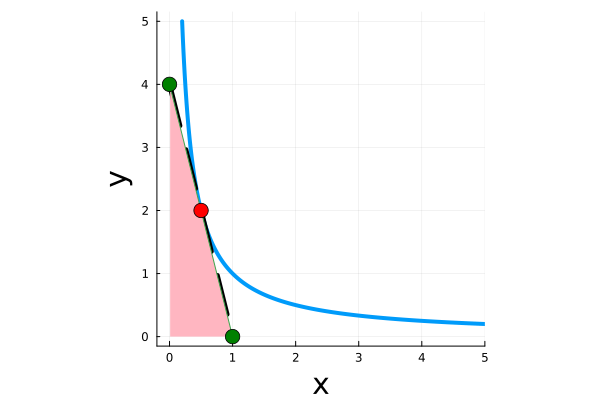
\includegraphics[width=0.33\columnwidth]{graphics/Chap05/WhatsSpecialAboutOneOverXhalf.png}}%
\hfill
\subfloat[]{%
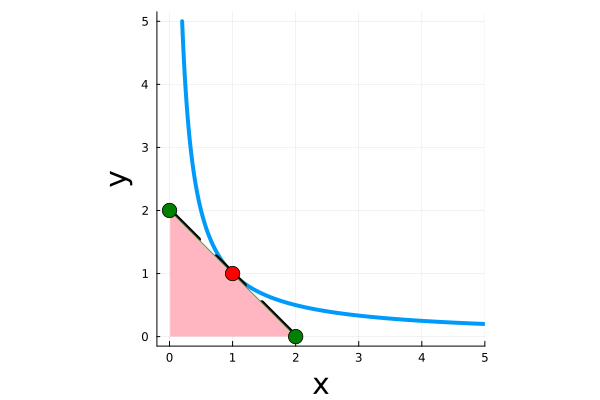
\includegraphics[width=0.33\columnwidth]{graphics/Chap05/WhatsSpecialAboutOneOverXone.png}}%
\hfill
\subfloat[]{%
\hfill
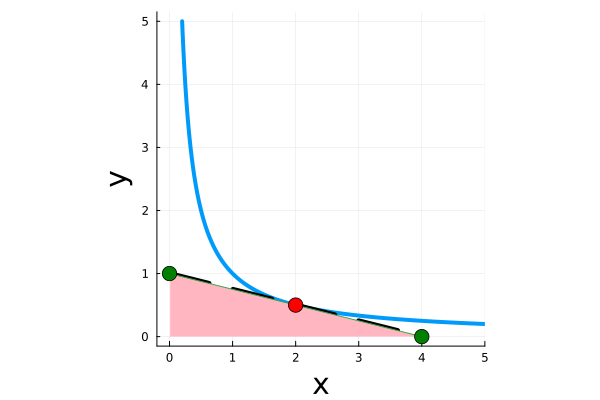
\includegraphics[width=0.33\columnwidth]{graphics/Chap05/WhatsSpecialAboutOneOverXtwo.png}}%
\hfill
    \caption[]{The blue line is the graph of $\frac{1}{x}$. The black dashed line is tangent to the red dot. The two green dots are the $x$- and $y$-intercepts for the tangent line. The pink triangle is the area between the tangent line and the $(x,y)$-axes. Its area is the same for all choices of the tangent point. \href{https://youtu.be/Nq6E8EeePVk}{Why the area under the tangent line of $1/x$ is special} by \bprp. }
    \label{fig:AreaAlwaysTwo}
\end{figure}

\vspace*{.2cm}

\begin{example} Compute the area highlighted in Fig.~\ref{fig:AreaAlwaysTwo}.
    
\end{example}
\textbf{Solution:} The formula for the tangent line is precisely the linear approximation of $f(x)=\frac{1}{x}$ at a point $x_0=a$. Hence, from \eqref{eq:AffineScalarApprox05},
$$y = f(a) + f'(a) \cdot (x - a).$$
Because $f'(x) =-\frac{1}{x^2}$, we arrive at 
$$y = \frac{1}{a} - \frac{1}{a^2} (x - a) =  \frac{2}{a} - \frac{1}{a^2} x. $$
Hence, the $y$-intercept of the line is the point $(0, \frac{2}{a})$ and the $x$-intercept is the point $(2a, 0)$. The area of the triangle is
$$\frac{1}{2} b \cdot h = \frac{1}{2} \cdot 2a \cdot  \frac{2}{a} = 2,$$
independent of the choice of $a>0$. 

\Qed

\vspace*{.2cm}




\section{Use Cases of the Single-variable Derivative}

That's really all the theory for derivatives of a function depending on a single variable. Before moving on to multivariable functions, we illustrate why derivatives are such a useful tool.





\begin{figure}[htb]%
\centering
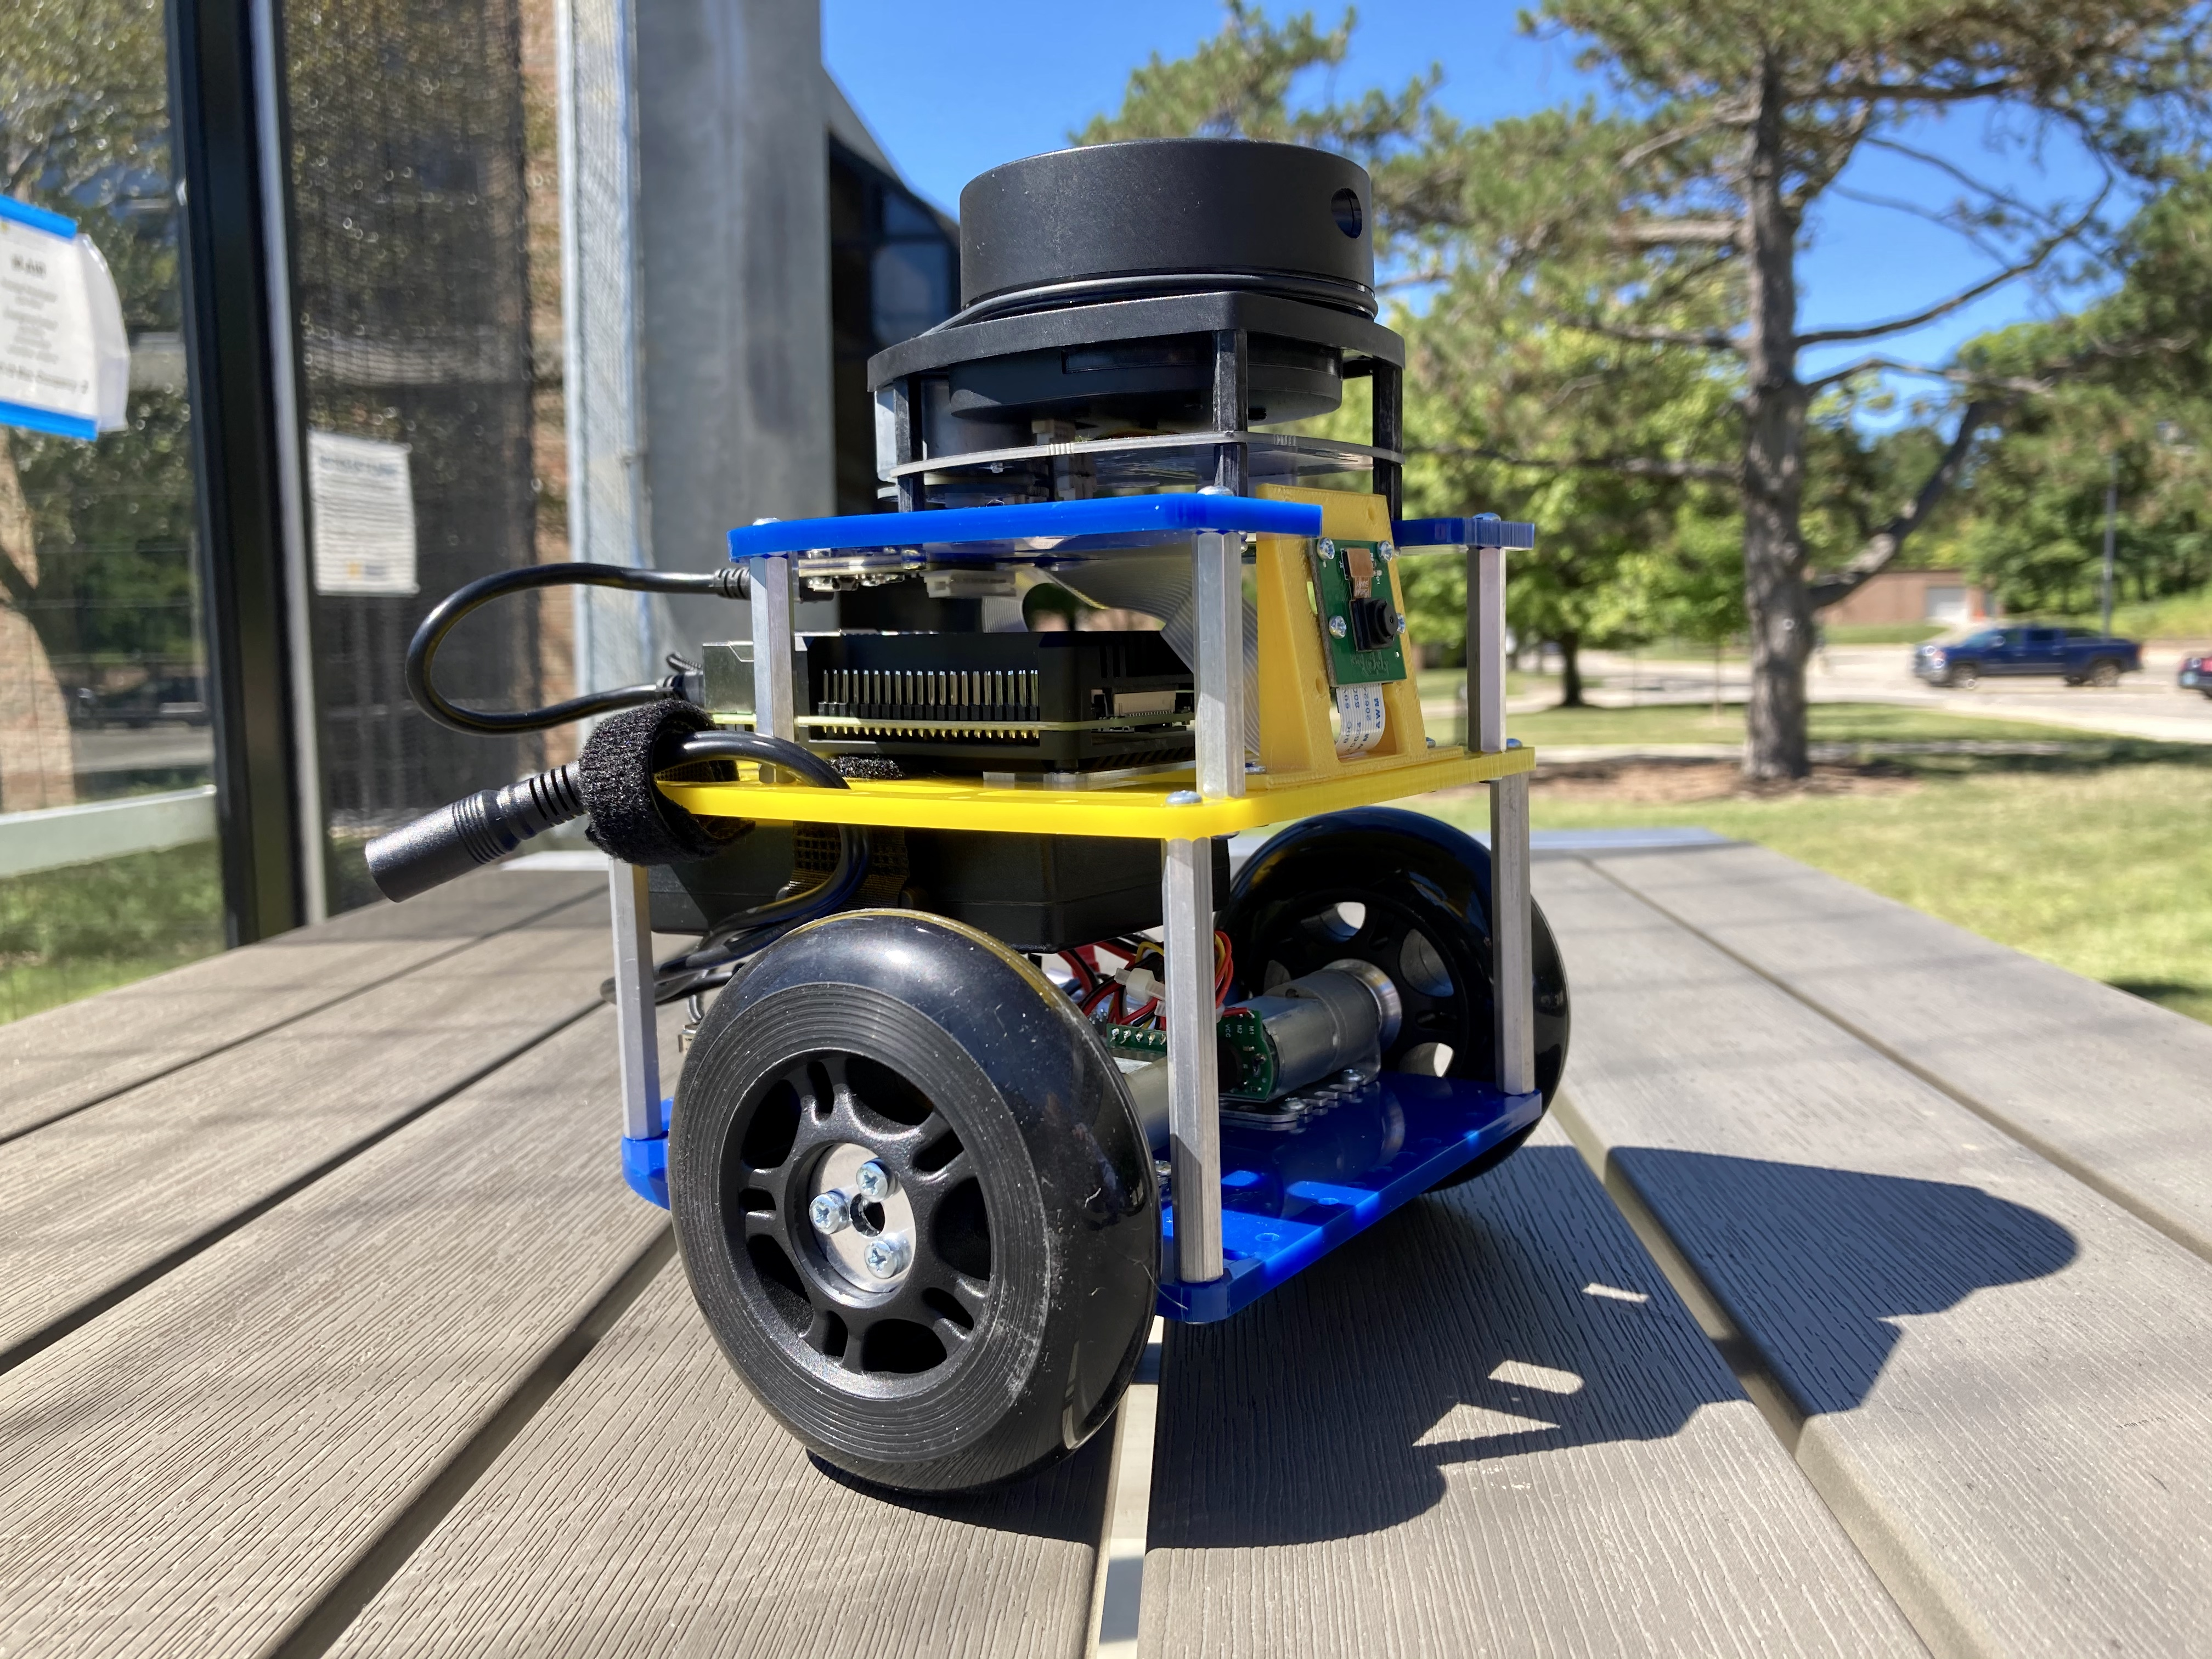
\includegraphics[width=0.6\columnwidth]{graphics/Chap03/MBotROB330.jpeg}%
    \caption[]{The same small mobile robot that we showed in Chapter~\ref{sec:Speed2ChangePosition}. The user commands wheel speed. If both wheels move at the same speed, the robot moves in a straight line. If one wheel turns faster than the other, the robot turns toward the side of the slower wheel. Yet, somehow, our ``Planning Team'' has given us position trajectories (aka, position curves in $\real^2$), instead of velocity. We need to convert the position trajectories to velocity commands because our ``Control Team'' is still working on the position trajectory tracking controller for the robot. It will not be available until Chapter~\ref{chap:LaplaceTransformFeedbackControl}.}
    \label{fig:MbotRoboticsChap05}
\end{figure}

\begin{figure}[htb]%
\centering
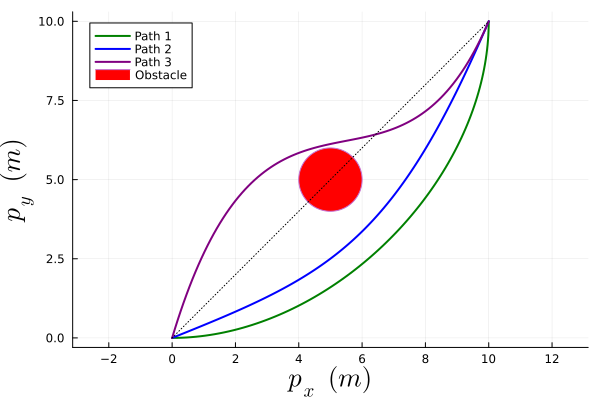
\includegraphics[width=0.6\columnwidth]{graphics/Chap05/MobileRobotPositionTrajectory.png}%
    \caption[]{The Planning Team has proposed the indicated paths for the robot to follow, each of which avoids the obstacle indicated in red. As explained in Fig.~\ref{fig:MbotRoboticsChap05}, our robot accepts the velocity of the paths. We can use Calculus to convert the paths to velocity commands because velocity is the (time) rate of change of position. Hence, $v(t) = \frac{d}{dt} p(t)$.}
    \label{fig:MobileRobotPositionTrajectory}
\end{figure}

%\clearpage
\subsection{From Position to Velocity}

The Planning Team of our company, \company, has given us the paths in $\real^2$ shown in Fig.~\ref{fig:MobileRobotPositionTrajectory}. Each path gets us from 
$${\rm Point~ A}= \left[
\begin{array}{c}
0 \\
0 \\
\end{array}
\right]  \text{ to } {\rm Point~ B}= \left[
\begin{array}{c}
10 \\
10 \\
\end{array}
\right],$$ 
while avoiding the obstacle shown in red. Good job, Planning Team! Shown by a dotted black line is a straight line connecting the two points, which goes right through the obstacle and would destroy the robot. That's why we called on the Planning Team for help! Our job is the following:

\begin{center}
\setlength{\fboxrule}{2pt}  % Setting the thickness of the border line
   \fbox{ \parbox{0.9\linewidth}{\textcolor{blue}{\bf {\large Task:} Select the path that has the \textbf{lowest peak speed so as to minimize the chance of the wheels slipping while maneuvering}}, where \textcolor{red}{\bf speed is defined to be the Euclidean norm of the velocity vector.} At each point in time, velocity has $x$- and $y$-components, making it a 2-vector. The norm is $$|| (v_x, v_y)|| = \sqrt{(v_x)^2 + (v_y)^2}.$$
   }
} 
\end{center}

Yep, we have one task, but to complete it, we have to do several things
\begin{enumerate}
\renewcommand{\labelenumi}{(\alph{enumi})}
\setlength{\itemsep}{.2cm}
    \item Have the Planning Team send us the equations for the position curves, parameterized by time; once again, they just sent us a plot of $p_{y}$ versus $p_{x}$; we want the actual functions of time.  
    \item Differentiate the position curves (functions) to obtain velocity. 
    \item Compute the instantaneous speed of each curve from the instantaneous velocity.
    \item Search over the speed curves to find the peak speed.
    \item Choose the best curve for our robot, the one that demands the lowest peak speed (thereby inducing the least chance of wheel slippage). 
\end{enumerate}

\vspace*{.2cm}

Below are the formulas that were finally sent to us. They are a little awkward, but Julia will not care. 
\begin{equation}
\label{eq:PositionTrajectories}
\begin{aligned}
   {\rm path}_1(t) &= \left[
\begin{array}{c}
0.37500000 t - 0.00007813 t^3 \\
0.00937500 t^2 - 0.00007813 t^3 \\
\end{array}
\right]\\
%%
{\rm path}_2(t) &=  \left[
\begin{array}{c}
 - 0.00562500 t^2 + 0.37500000 t + 0.00006250 t^3 \\
 - 0.00187500 t^2 + 0.15000000 t + 0.00010938 t^3 \\
\end{array}
\right]\\
%
%
{\rm path}_3(t)&= \left[
\begin{array}{c}
0.00187500 t^2 + 0.22500000 t - 0.00003125 t^3 \\
 - 0.03187500 t^2 + 0.75000000 t + 0.00048438 t^3 \\
\end{array}
\right].
\end{aligned}
\end{equation}

Next, we place the functions in Julia and do the rest of the work there. Why? Because differentiating the polynomials line by line using the Power Rule is now too easy for you. And because doing the work in code provides documentation that we can share with other members of \company.


\begin{lstlisting}[language=Julia,style=mystyle]
# Paths from the Planning Team
using LinearAlgebra
@variables t

path1 = [0.375t - 7.812500000000002e-5(t^3), 
    0.009375000000000001(t^2) - 7.812500000000002e-5(t^3)]

path2 = [0.375t + 6.250000000000001e-5(t^3) - 0.0056250000000000015(t^2), 
    0.15000000000000002t + 0.00010937500000000003(t^3) - 0.0018750000000000004(t^2)]

path3 = [0.0018750000000000004(t^2) + 0.225t - 3.125000000000001e-5(t^3), 
    0.75t + 0.0004843750000000001(t^3) - 0.03187500000000001(t^2)]

# Derivatives of the paths
v1 = deriv(path1, t)
v2 = deriv(path2, t)
v3 = deriv(path3, t)

# Range of t values
t_values = collect(0:0.01:40)


v1_traj = evaluate(v1, t_values)
v2_traj = evaluate(v2, t_values)
v3_traj = evaluate(v3, t_values)

# The rows are indexed by time. We want to apply 
# norm to the columns. That is easy to do in Julia
speed_1 = norm.(eachcol(v1_traj))
speed_2 = norm.(eachcol(v2_traj))
speed_3 = norm.(eachcol(v3_traj))

# Compute max speeds
@show maximum(speed_1)
@show maximum(speed_2)
@show maximum(speed_3)

# Make Speed Plots vs time

# Define an array of colors
colors = [:green, :blue, :purple, :orange]  

plot1=plot(t_values, speed_1, linewidth=2, linecolor=colors[1], label="Speed 1", 
    xlabel=L"$t ~~(s)$", ylabel=L"$Speed ~~(m/s)$",
    yguidefontsize=18, xguidefontsize=18)
plot1=plot!(t_values, speed_2, linewidth=2, linecolor=colors[2], label="Speed 2")
plot1=plot!(t_values, speed_3, linewidth=2, linecolor=colors[3], label="Speed 3")

display(plot1)
png(plot1, "MobileRobotSpeeds")
\end{lstlisting}
\textbf{Output} 
\begin{verbatim}
maximum(speed_1) = 0.39774756441743303
maximum(speed_2) = 0.5711829829397932
maximum(speed_3) = 0.7830229881682913
\end{verbatim}

\begin{center}
    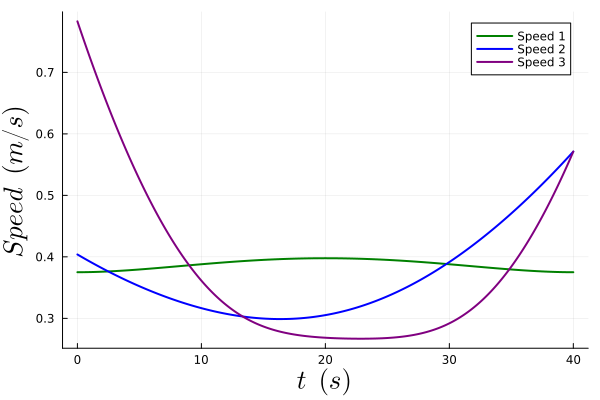
\includegraphics[width=0.45\columnwidth]{graphics/Chap05/MobileRobotSpeeds.png}
\end{center}

\vspace*{.2cm}

\begin{center}
\setlength{\fboxrule}{2pt}  % Setting the thickness of the border line
   \fbox{ \parbox{0.9\linewidth}{\textcolor{red}{\bf \large Conclusion:} Each of the paths gets us from Point A to Point B in 40 seconds. {\bf Path 1 is the best by our criterion of lowest peak speed.} All of them will likely work. We can give props to the Planning Team!
}
}
\end{center}

\vspace*{.2cm}

Here is the ``upgraded'' \texttt{evaluate} function, using Julia's multiple dispatch feature.

\begin{lstlisting}[language=Julia,style=mystyle]
# evaluate has here been extended to use multiple dispatch

# Method when f is a symbolic expression and x0 is a Float64
function evaluate(f::Any, x0::Float64)
    vars = Symbolics.get_variables(f)
    return Symbolics.value(substitute(f, (Dict(first(vars) => x0))))
end

# Method when f is a function and x0 is a Float64
function evaluate(f::Function, x0::Float64)
    return f(x0)
end

# Method when f is a vector of symbolic expressions and x0 is a vector of Float64                
function evaluate(f::Vector{Any}, x0::Vector{Float64})
    vars = Symbolics.get_variables(f[1])
    var = first(vars)
    return hcat([float.(Symbolics.value.(substitute.(f, Ref(var => x_val)))) for x_val in x0]...)
end                

    
# Method when f is a vector of symbolic expressions and x0 is a vector of Float64                
function evaluate(f::Vector{Num}, x0::Vector{Float64})
    vars = Symbolics.get_variables(f[1])
    var = first(vars)
    return hcat([float.(Symbolics.value.(substitute.(f, Ref(var => x_val)))) for x_val in x0]...)
end 

# Method when f is a vector of functions and x0 is a vector of Float64
function evaluate(f::Vector{Function}, x0::Vector{Float64})
    return [fi(xi) for (fi, xi) in zip(f, x0)]
end
      
\end{lstlisting}
\textbf{Output} 
\begin{verbatim}
evaluate (generic function with 5 methods)
\end{verbatim}

\begin{funColor}{Taking Stock: Relations between Differentiation and Integration}{RelationsDifferentiationIntegration}

In the above, we differentiated with respect to time the $(x,y)$-coordinates of a position trajectory and obtained a velocity profile as a function of time. Back in Chapter~\ref{sec:Speed2ChangePosition}, we did the opposite: we started with $(x,y)$-coordinates of a velocity profile and integrated them to obtain position trajectories.  In symbols, this is what we have done,
\begin{equation}
\label{eq:RelationsDifferentiationIntegration}
\begin{aligned}
 v(t) &= \begin{bmatrix} v_x(t) \\ v_y(t) \end{bmatrix} = \begin{bmatrix} \frac{d p_x(t)}{dt} \\ \frac{d p_y(t)}{dt} \end{bmatrix} \\[1em]  
    p(t) &= \begin{bmatrix} p_x(t) \\ p_y(t) \end{bmatrix} = 
    \begin{bmatrix} p_x(t_0) +  \int_{t_0}^t v_x(\tau) d\tau\\[0.5em]  
    p_y(t_0) + \int_{t_0}^t v_y(\tau) d\tau\end{bmatrix}.   
\end{aligned}    
\end{equation}
In other words, it seems that we can go back and forth in the sense that
\begin{itemize}
    \item If we apply the differentiation operator to a function (or vector of functions), we can ``undo it'' via integration; and 
    \item if we apply the integration operator to a function (or vector of functions), we can ``undo it'' via differentiation.
\end{itemize}
In plain words, one operation is the inverse of the other! This is remarkable. Differentiation takes a very local view of a function to extract its slope at a point, while definite integration focuses on an arbitrarily large (but bounded) region of the function's domain to compute the area under the function. \\

One possibility is that this is simply an accident of physics (F = ma), and for more general functions, the inverse relationships between differentiation and integration fall apart. Another possibility is that they hold very broadly. Which is it?\\

Chapter~\ref{chap:AntiDerivFundThmCalc} shows that the inverse relationships between differentiation and integration hold very broadly. Moreover, these relationships will give us a new way of computing integrals. There is lots of cool stuff to come!    
\end{funColor}

\begin{table}[ht]
\centering
\begin{tabular}{lcc}
\toprule
Function ($f(x)$) & Derivative ($f'(x)$) & Monotonicity \\
\midrule
$x^3$ & $3x^2$ & Strictly Increasing \\
$-x^3$ & $-3x^2$ & Strictly Decreasing \\
$\ln(x)$ & $\frac{1}{x}$ & Strictly Increasing for $x > 0$ \\
$e^x$ & $e^x$ & Strictly Increasing \\
$e^{-x}$ & $-e^{-x}$ & Strictly Decreasing \\
$\tan(x)$ & $1 + \tan^2(x)$ & Strictly Increasing (in its domain) \\
$\frac{1}{1 + x^2}$ & $-\frac{2x}{(1+x^2)^2}$ & Strictly Decreasing for $x \ge  0$ \\
\addlinespace
$\frac{1}{1 + x^2}$ & $-\frac{2x}{(1+x^2)^2}$ & Strictly Increasing for $x \leq 0$ \\
\addlinespace
$\frac{x^2}{x^2 + 1}$ & $\frac{2x}{(x^2+1)^2}$ & Strictly Increasing for $x \ge  0$\\
\bottomrule
\end{tabular}
\caption{Monotonicity of functions through the lens of their derivatives.}
\label{tab:Monotonicity}
\end{table}

\subsection{If the Derivative does not Change Sign, the Function is Monotonic}
\label{sec:DerivativeAndMonotonicity}

In Chapter~\ref{sec:MonotonicFunctionsAndInverseFunctions}, we learned that a strictly monotonic function (increasing or decreasing) has an inverse as long as the codomain of the function has been chosen properly (it must equal the function's range). We address here how to use a function's derivative to check monotonicity, both strict and non-strict.

Let $I \subset \real$ be an open interval and let $f:I \to \real$ be a function on $I$. For convenience, we recall the various forms of monotonicity:
\begin{itemize}
    \item $f$ is \textbf{nondecreasing} if $y > x \implies f(y) \ge f(x)$;
    \item $f$ is \textbf{strictly increasing} if $y > x \implies f(y) > f(x)$. Similarly, 
    \item $f$ is \textbf{nonincreasing} if $x < y\implies f(x) \le f(y)$;
    \item $f$ is \textbf{strictly decreasing} if $x < y\implies f(x) < f(y)$. 
    \item \textbf{Note:} A constant function is both nondecreasing and nonincreasing but is neither strictly increasing nor strictly decreasing.     
\end{itemize}

\vspace*{.2cm}

\begin{propColor}{Monotonic Functions}{Monotonicity}
Let $I \subset \real$ be an open interval and let $f:I \to \real$ be a differentiable function on $I$. The following statements are true. 
\begin{enumerate}
\renewcommand{\labelenumi}{(\alph{enumi})}
\setlength{\itemsep}{.2cm}
    \item If $\frac{df(x)}{dx} \ge 0$ for all $x\in I$, then $f$ is nondecreasing.
    \item If $\frac{df(x)}{dx} \le 0$ for all $x\in I$, then $f$ is nonincreasing.
    \item If $\frac{df(x)}{dx} > 0$ for all $x\in I$, then $f$ is strictly increasing.
    \item If $\frac{df(x)}{dx} < 0$ for all $x\in I$, then $f$ is strictly decreasing.
\end{enumerate}

The last two statements can be relaxed just a bit. 
\begin{enumerate}
\renewcommand{\labelenumi}{(\alph{enumi})}
\setlength{\itemsep}{.2cm}
    \item[(c')] If $\frac{df(x)}{dx} =0 $ for a finite number of $x\in I$ and  $\frac{df(x)}{dx} > 0 $ elsewhere, then $f$ is strictly increasing.
    \item[(d')] If $\frac{df(x)}{dx} =0 $ for a finite number of $x\in I$ and  $\frac{df(x)}{dx} < 0 $ elsewhere, then $f$ is strictly decreasing.
\end{enumerate}
These ``friendly amendments'' are important for a function such as $x^3$, where the derivative $3 x^2$  vanishes at the origin. Otherwise, you would be saying the function is strictly increasing on $(-\infty, 0)$ and $(0, \infty)$, and be perplexed about what is happening for $x=0$. That would not be good!    
\end{propColor}

\vspace*{.2cm}

Several examples of Prop.~\ref{thm:Monotonicity} are given in Table~\ref{tab:Monotonicity}. Traditionally, a proof of Prop.~\ref{thm:Monotonicity} is based on the Fundamental Theorem of Calculus, developed later in the book. Fortunately for us, the limit definition of a derivative provides good insight into why it is true! Indeed, consider
$$\frac{df(x)}{dx} = \lim_{h \to 0^+} \frac{f(x+h) -f(x)}{h},$$
where $x+h >x$ plays the role of $y>x$ because $h$ is greater than zero when we take the limit from the right. For the derivative to be strictly greater than zero at $x$, it must be true that $f(x+h) > f(x)$. And then $f(x+2h) > f(x +h)$ follows from $\frac{df(x+h)}{dx} >0$, and so forth. While this reasoning is only qualitative, you get the idea. 




\begin{funColor}{Once Upon A Time ...}{PurchaseLHopitalRule}
   {\bf ...} you could purchase mathematical results and claim them as your own! L'H\^opital's Rule is named for the French mathematician Guillaume-François-Antoine, Marquis de L'H\^opital, who purchased the formula from his teacher, the Swiss mathematician Johann Bernoulli. Recall that the number $e$ was discovered by the Swiss mathematician Jacob Bernoulli. They were \href{https://en.wikipedia.org/wiki/Bernoulli_family#:~:text=In%20addition%20to%20Jacob%20and,%E2%80%931726)%2C%20son%20of%20Johann}{brothers}. Can you imagine buying some math results to improve your standing in society? \\

   \textbf{Note:} L'H\^opital is also spelled L'Hospital. In French, the circumflex is used to indicate that an ``s'' has been dropped. The circumflex is also present in the French word ``h\^otel'', which we use in English as ``hotel'', but we also have ``hostel'', as in a ``Youth Hostel''. The ways we have incorporated French into English can be very confusing. One example: the French word ``entr\'ee'' means ``starter'' or ``appetizer'' on a ``carte (menu)'' in France. We, of course, use it as ``plat principal'', aka the main dish. Yikes!
\end{funColor}


\subsection{L'H\^opital's Rule for Evaluating Limits}

L'H\^opital's Rule is a powerful tool used to evaluate limits that take the form $\frac{0}{0}$ or $\frac{\pm \infty}{\pm \infty}$. Such forms are called \textbf{indeterminate}. Named after the French mathematician Guillaume de l'H\^opital, this rule simplifies the process of finding such limits by differentiating the numerator and the denominator of the function.

\begin{propColor}{L'H\^opital's Rule}{LHopitalRule}
Let $I:=(a, b)$ be an open interval, $x_0 \in I$ a point in $I$, and $f:I \to \real$ and $g:I \to \real$ two functions that are differentiable on $I$ except possibly at $x_0$. If $f$ and $g$ satisfy the additional conditions,

\begin{enumerate}
\renewcommand{\labelenumi}{(\alph{enumi})}
\setlength{\itemsep}{.2cm}
    \item  For all $x\in I$, $x \neq x_0$, $g'(x) \neq 0$.
    \item  $\displaystyle \lim_{x \to x_0} f(x) = \lim_{x \to x_0} g(x) = 0$ or $ |\lim_{x \to x_0} f(x)| = | \lim_{x \to x_0} g(x)| = \infty$ (means the limits of $f$ and $g$ can be $\pm \infty$).
    \item   $\displaystyle \lim_{x \to x_0} \frac{f'(x)}{g'(x)}$ exists  (can be finite or infinite, but it must exist).
    \end{enumerate}
    Then, 
    \begin{equation}
        \label{eq:LhoptialRule}
        \lim_{x \to x_0} \frac{f(x)}{g(x)} = \lim_{x \to x_0} \frac{f'(x)}{g'(x)}.
    \end{equation}

    \textbf{Notes:} 
    \begin{itemize}
        \item In the above we have expressed the result using two-sided limits. It also works for one-sided limits, $x \to x_0^-$ or $x \to x_0^+$, and for $x \to \pm \infty$.
        \item What if $\displaystyle \lim_{x \to x_0} \frac{f'(x)}{g'(x)}$ is also indeterminate? Then you can apply L'H\^opital's Rule to $\frac{f'(x)}{g'(x)}$ and work with the second derivatives, $\frac{f''(x)}{g''(x)}$, etc. This can go on until you run out of steam or get an answer. Usually, one application suffices.
    \end{itemize}
\end{propColor}

\vspace*{.2cm}

\begin{example} Consider the function $ \frac{\sin(x)}{x} $ as $ x $ approaches 0. Both the numerator and the denominator approach 0, placing us in the indeterminate form $\frac{0}{0}$. Can we apply L'Hôpital's Rule?
\end{example}

\solution Differentiating the numerator (aka, $f(x) = \sin(x)$), we obtain $ \cos(x) $, and differentiating the denominator (aka, $g(x) = x$), yields 1, which is non-zero. Therefore, the limit becomes,
$$
\lim_{{x \to 0}} \frac{\cos(x)}{1} = \cos(0) = 1.
$$
Because all the conditions for L'H\^opital's Rule are met, we conclude
$$
\lim_{{x \to 0}} \frac{\sin(x)}{x} = \lim_{{x \to 0}} \frac{\cos(x)}{1} = \cos(0) = 1.
$$    

\Qed


\textbf{Bottom line:} L'H\^opital's Rule is a convenient method for evaluating limits of indeterminate forms. It saves time and simplifies the process by allowing us to differentiate the numerator and the denominator to find the limit. \\

Another \textbf{indeterminate form } is $0 \cdot \infty$. Can  L'H\^opital's Rule help there as well? Yes, because we can rewrite it in the standard form treated in Prop.~\ref{thm:LHopitalRule}, as we illustrate next.

\vspace*{.2cm}

\begin{example} Determine the following limits.

\begin{enumerate}
\renewcommand{\labelenumi}{(\alph{enumi})}
\setlength{\itemsep}{.2cm}

    \item $\displaystyle \lim_{{x \to \infty}} x e^{-x}$.
   
    
    \item $\displaystyle \lim_{{x \to \infty}} \frac{x^2 + 3x + 2}{2x^2 + 4x + 1}$


    \item $\displaystyle \lim_{{x \to 0}} \frac{\ln(1+x)}{x}$

    \item $\displaystyle \lim_{{x \to \infty}} x \ln\left(\frac{1}{x}\right)$


\item $\displaystyle \lim_{{x \to 0}} \frac{e^x - \cos(x)}{x}$

\end{enumerate}   

\textbf{Note:} The first two problems can be solved using the results of Chapter~\ref{sec:LimitInfinityEasy} and Chapter~\ref{sec:ExponentialGrowth}. It's good to see them through the lens of L'H\^opital. Part (d) of the problem could \textcolor{red}{\bf easily trip you up}. Definitely take a look at it for yourself before reading the solutions.
    
\end{example}

\textbf{Solutions:}

\begin{enumerate}
\renewcommand{\labelenumi}{(\alph{enumi})}
\setlength{\itemsep}{.2cm}

    \item \Ans $\displaystyle \lim_{{x \to \infty}} x e^{-x} =0$.\\

    This problem has the indeterminate form $\infty \cdot 0$. We rewrite it in the form $\frac{\infty}{\infty}$, via
 \begin{align*}
     \lim_{{x \to \infty}} x e^{-x} &= \lim_{{x \to \infty}} \frac{x}{e^{x}} ~~ (\text{reciprocal property of exponentials})\\
     &=  \lim_{{x \to \infty}} \frac{1}{e^{x}}~~(\text{differentiate numerator and denominator})\\
     &= 0.
 \end{align*}

    We could have also rewritten it in the form  $\frac{0}{0}$, but as you will see, it leaves us with a harder problem to solve in this case. In other problems, the opposite is true. Hence, there is ``art'' in the application of mathematical tools! And thank goodness for that! Because if there weren't any art involved (aka, you could just turn a crank), a bot could easily take our jobs as engineers.

   \begin{align*}
     \lim_{{x \to \infty}} x e^{-x} &= \lim_{{x \to \infty}} \frac{e^{-x}}{\frac{1}{x}} ~~ (x = \frac{1}{1/x})\\
     &=  \lim_{{x \to \infty}} \frac{-e^{-x}}{\frac{-1}{x^2}}~~(\text{differentiate numerator and denominator})\\
     &= ~\text{a mess!}
 \end{align*}  

    
   
    \item \Ans $\displaystyle \lim_{{x \to \infty}} \frac{x^2 + 3x + 2}{2x^2 + 4x + 1} = \frac{1}{2}$\\

    This problem uses L'H\^opital's Rule twice. Its indeterminate form is $\frac{\infty}{\infty}$, so it falls directly into the L'H\^opital framework.
\begin{align*}
     \lim_{{x \to \infty}} \frac{x^2 + 3x + 2}{2x^2 + 4x + 1} &=   \lim_{{x \to \infty}} \frac{2x+3}{4x + 4}~~ (\text{differentiate numerator and denominator})\\
     &=  \lim_{{x \to \infty}} \frac{2}{4}~~(\text{differentiate numerator and denominator once more})\\
     &= \frac{1}{2}.
\end{align*}


    
    \item \Ans $\lim_{{x \to 0}} \frac{\ln(1+x)}{x} = 1$. \\

    The indeterminate form of this problem is $\frac{0}{0}$, so it falls directly into the L'H\^opital framework.
 
\begin{align*}
     \lim_{{x \to 0}} \frac{\ln(1+x)}{x}&=   \lim_{{x \to 0}} \frac{\frac{1}{x+1}}{1}~~ (\text{differentiate numerator and denominator})\\
     &=  1.
\end{align*}
    

\item \Ans $\displaystyle \lim_{{x \to \infty}} x \ln\left(\frac{1}{x}\right) = -\infty$.\\

\textcolor{red}{\bf This is not an indeterminate form\footnote{Plus infinity times minus infinity is not indeterminate. To be indeterminate, we need $\frac{0}{0}$ or $\frac{\pm \infty}{\pm \infty}$.}, and thus L'H\^opital's Rule does not apply.} It is still valid to assign $f(x) := x$ and $g(x) := \ln\left(\frac{1}{x}\right)$. Then, we note,
\begin{align*}
    \lim_{{x \to \infty}} f(x) & = \lim_{{x \to \infty}} x\\
    &= \infty\\
    \\
 \lim_{{x \to \infty}} g(x) & = \lim_{{x \to \infty}} \ln\left(\frac{1}{x}\right) \\
 &= \lim_{{x \to \infty}} -\ln\left(x\right) ~~(\text{logarithm rules})\\
    &= - \infty.    
\end{align*}
Hence, 
$$\lim_{{x \to \infty}} f(x) \cdot g(x) = -\infty,$$
because something large and positive times something large and negative is something (super) large and negative.\\

\emstat{Now, suppose we skipped the above analysis and applied L'H\^opital's Rule \textcolor{red}{\bf \large blindly!} We might do something like this
\begin{align*}
     \lim_{{x \to \infty}} x \ln\left(\frac{1}{x}\right) & =  \lim_{{x \to \infty}} \frac{\ln\left(\frac{1}{x}\right)}{\frac{1}{x}} ~~ (x = \frac{1}{1/x}) \\
     &= \lim_{{x \to \infty}} \frac{x \cdot \frac{-1}{x^2}}{\frac{-1}{x^2}} ~~(\text{differentiate numerator and denominator with the Chain Rule}) \\
     &= \lim_{{x \to \infty}} x ~~(\text{cancel like terms in the numerator and denominator}) \\
     & = \infty.
\end{align*}
That means we blew the sign on the limit! Or, we might even say, our error is $-2 \cdot \infty$ ($-\infty - \infty$, actual limit minus computed limit). Crazy! But, that is what happens when you misapply L'Hopital's Rule, as ChatGPT4 did for your author! You gotta be careful.}


Here is another VALID solution using logarithm rules.
\begin{align*}
     \lim_{{x \to \infty}} x \ln\left(\frac{1}{x}\right) & =  \lim_{{x \to \infty}} x \cdot \left( \ln(1) - \ln(x) \right) ~~ (\ln(a/b) = \ln(a) - \ln(b))\\
     &= \lim_{{x \to \infty}} -x \cdot \ln(x)~~(\ln(1) = 0) \\
     & = -\infty,
\end{align*}
because, $\displaystyle \lim_{{x \to \infty}} x = \infty$ and $\displaystyle \lim_{{x \to \infty}} \ln(x) = \infty$.

\item \Ans $\displaystyle \lim_{{x \to 0}} \frac{e^x - \cos(x)}{x} = 1$\\

This problem's indeterminate form is $\frac{0}{0}$, so it falls directly into the L'H\^opital framework.
\begin{align*}
      \lim_{{x \to 0}} \frac{e^x - \cos(x)}{x} &=   \lim_{{x \to 0}} \frac{e^x + \sin(x)}{1}~~ (\text{differentiate numerator and denominator})\\
     &=  1.
\end{align*}
\end{enumerate}    

\Qed


% \begin{rem}
%     All four conditions for L'H\^opital's rule are \textbf{necessary} (from \href{https://en.wikipedia.org/wiki/L%27H%C3%B4pital%27s_rule#:~:text=Cases%20where%20theorem%20cannot%20be%20applied%20(Necessity%20of%20conditions)}{Wikipedia}):
% \begin{itemize}

% \item \textbf{Indeterminacy of form:} $\displaystyle \lim_{x \to x_0} f(x) = \lim_{x \to x_0} g(x) = 0 $ or $\pm \infty $; 
% \item \textbf{Differentiability of functions:} $f(x) $and $g(x) $are differentiable on an open interval $I$ except possibly at a point $x_0$ contained in $I$ (the same point used in the limit); 
% \item \textbf{Non-zero derivative of denominator:} $g'(x) \ne 0 $ for all $x $ in $I$ with $x \ne x_0 $; and
% \item \textbf{Existence of limit of the quotient of the derivatives:} $\displaystyle \lim_{x \to x_0} \frac{f'(x)}{g'(x)}$ exists.
% \end{itemize}
% {\bf If even one of the above conditions is not satisfied, L'H\^opital's rule is not valid} \textcolor{red}{\bf (i.e., it CANNOT be applied)}.
%  \end{rem} 

 \begin{factColor}{Need to Apply  L'H\^opital's Rule with Care}{lhopitalRulesNecessity}
         All four conditions for L'H\^opital's rule are \textbf{necessary} (from \href{https://en.wikipedia.org/wiki/L%27H%C3%B4pital%27s_rule#:~:text=Cases%20where%20theorem%20cannot%20be%20applied%20(Necessity%20of%20conditions)}{Wikipedia}):
\begin{itemize}

\item \textbf{Indeterminacy of form:} $\displaystyle \lim_{x \to x_0} f(x) = \lim_{x \to x_0} g(x) = 0 $ or $\pm \infty $; 
\item \textbf{Differentiability of functions:} $f(x)$ and $g(x) $are differentiable on an open interval $I$ except possibly at a point $x_0$ contained in $I$ (the same point used in the limit); 
\item \textbf{Non-zero derivative of denominator:} $g'(x) \ne 0 $ for all $x $ in $I$ with $x \ne x_0 $; and
\item \textbf{Existence of limit of the quotient of the derivatives:} $\displaystyle \lim_{x \to x_0} \frac{f'(x)}{g'(x)}$ exists.
\end{itemize}
{\bf If even one of the above conditions is not satisfied, L'H\^opital's rule is not valid} \textcolor{red}{\bf (i.e., it CANNOT be applied)}.
 \end{factColor}
 

\vspace*{.2cm}

\begin{example} Compute $\displaystyle \lim_{x \to \infty} \sqrt[x]{x}$.
    
\end{example}
\textbf{Solution:} \href{https://www.youtube.com/shorts/2V9BkfIoqv8?feature=share}{1 in 1 Minute} by \bprp (do not hesitate to adjust the playback speed).
\Qed

\begin{center}
\setlength{\fboxrule}{2pt}  % Setting the thickness of the border line
   \fbox{ \parbox{0.9\linewidth}{
   \textcolor{blue}{\bf \large Want more examples?} \bf
   \begin{itemize}
       \item \href{https://www.youtube.com/watch?v=tsptFBqf2Ug}{L'H\^ opital's Rule: Ultimate Study guide} by \bprp
       \item \href{https://youtu.be/Gh48aOvWcxw}{L'Hopital's rule} by The Organic Chemistry Tutor.
       \item \href{https://youtu.be/uhxGH7OhrIM}{What is L'Hospital's rule?} by \href{https://www.kristakingmath.com/about-krista}{Krista King}. (She also talks about Johann Bernoulli.)
   \end{itemize}
} % close parbox
}  % close fbox
\end{center}




\rule{\linewidth}{2.0pt}
\begin{lstlisting}[language=Julia,style=mystyle]
# Reminder about our function 

using Symbolics

# For scalar functions
function deriv(f::Symbolics.Num, x::Symbolics.Num)
    df = Differential(x)(f)
    return simplify(expand_derivatives(df))  # Note the simplify command
end

# For vector-valued functions
function deriv(f::Vector{Symbolics.Num}, x::Symbolics.Num)
    df = []
    for component in f
        df_comp = Differential(x)(component)
        push!(df, simplify(expand_derivatives(df_comp)))  # Note the simplify command
    end
    return df
end
\end{lstlisting}
\textbf{Output} 
\begin{verbatim}
deriv (generic function with 2 methods)
\end{verbatim}

\begin{lstlisting}[language=Julia,style=mystyle]
@variables x1 x2 x3

fa = [x1 * (x2)^2; exp(3*x1) + cos(4*x2)]
fb = exp(3*x1) + cos(4*x2) # not a vector, hence no brackets!
fc = [x1 * (x2)^2; x2*( sin(x1) )^3 + 11; 4*(x1)^2 + ( x2 +3 )^2]
fd = [x1*x2*(x3)^3; x2*exp(x1*x3); x1]



@show dfadx1 = deriv.(fa, x1)
@show dfadx2 = deriv.(fa, x2)
println(" ")
@show dfbdx1 = deriv.(fb, x1)
@show dfbdx2 = deriv.(fb, x2)
println(" ")
@show dfcdx1 = deriv.(fc, x1)
@show dfccx2 = deriv.(fc, x2)
println(" ")
@show dfddx1 = deriv.(fd, x1) # the dfddxi is really dfd/dxi
@show dfddx2 = deriv.(fd, x2)
@show dfddx3 = deriv.(fd, x3);
\end{lstlisting}
\textbf{Output} 
\begin{verbatim}
dfadx1 = deriv.(fa, x1) = Num[x2^2, 3exp(3x1)]
dfadx2 = deriv.(fa, x2) = Num[2x1*x2, -4sin(4x2)]
 
dfbdx1 = deriv.(fb, x1) = 3exp(3x1)
dfbdx2 = deriv.(fb, x2) = -4sin(4x2)
 
dfcdx1 = deriv.(fc, x1) = Num[x2^2, 3x2*(sin(x1)^2)*cos(x1), 8x1]
dfccx2 = deriv.(fc, x2) = Num[2x1*x2, sin(x1)^3, 2(3 + x2)]
 
dfddx1 = deriv.(fd, x1) = Num[x2*(x3^3), x2*x3*exp(x1*x3), 1]
dfddx2 = deriv.(fd, x2) = Num[x1*(x3^3), exp(x1*x3), 0]
dfddx3 = deriv.(fd, x3) = Num[3x1*x2*(x3^2), x1*x2*exp(x1*x3), 0]
\end{verbatim}
\Qed

\section*{Explaining the \texttt{Num} Type in Julia}

I asked ChatGpt4 to explain the \texttt{Num} Type in the expression \texttt{Num}$[x_2^2, 3 \cdot x_2 \cdot (\sin(x_1)^2) \cdot \cos(x_1), 8x1]$. Here's what it said. ``\textbf{Num: In the context of Julia and symbolic computation:} \texttt{Num} is a type that holds symbolic numbers or expressions. These are not evaluated until you explicitly ask Julia to do so. They can be variables, standard mathematical functions, or more complex expressions.'' ChatGPT4 did not say this, but it should have: {\bf The key thing is, you can continue taking derivatives like so},\\

\begin{lstlisting}[language=Julia,style=mystyle]
@show d2fadx1dx1 = deriv.(dfadx1 , x1)
@show d2fadx1dx2 = deriv.(dfadx1 , x2)
println(" ")
@show d2fadx2dx1 = deriv.(dfadx2 , x1)
@show d2fadx2dx2 = deriv.(dfadx2 , x2)
println(" ")
\end{lstlisting}
\textbf{Output} 
\begin{verbatim}
d2fadx1dx1 = deriv.(dfadx1, x1) = Num[0, 9exp(3x1)]
d2fadx1dx2 = deriv.(dfadx1, x2) = Num[2x2, 0]
 
d2fadx2dx1 = deriv.(dfadx2, x1) = Num[2x2, 0]
d2fadx2dx2 = deriv.(dfadx2, x2) = Num[2x1, -16cos(4x2)]
\end{verbatim}
where the correct mathematical notation would be
$$\frac{\partial^2 f_a(x_1, x_2)}{\partial x_1^2} = \frac{\partial^2 f_a(x_1, x_2)}{\partial x_1 \partial x_1} = \left[ \begin{array}{c}
        0\\ 9 e^{3 x_1}
    \end{array}\right] ~\text{ and } ~ \frac{\partial^2 f_a(x_1, x_2)}{\partial x_1 \partial x_2} = \left[ \begin{array}{c}
        2 x_2\\ 0
    \end{array}\right]$$

    $$ \frac{\partial^2 f_a(x_1, x_2)}{\partial x_2 \partial x_1} = \left[ \begin{array}{c}
        2 x_2\\ 0
    \end{array}\right] ~\text{ and } ~ \frac{\partial^2 f_a(x_1, x_2)}{\partial x_2^2} =\frac{\partial^2 f_a(x_1, x_2)}{\partial x_2 \partial x_2} = \left[ \begin{array}{c}
        2 x_1\\ -16 \cos(4 x_2)
    \end{array}\right].$$

And then you take derivatives of those expressions as well; see \href{https://youtu.be/BUIleGfqAeo}{Introduction to Higher Order Partial Derivatives Notation and Example} by the Math Sorcerer. \textbf{Our final remark here is the following:}

\begin{center}
\setlength{\fboxrule}{2pt}  % Setting the thickness of the border line
   \fbox{ \parbox{0.9\linewidth}{\textcolor{blue}{\bf Is it OK to use $\bm{\frac{\partial}{ \partial x_1}}$ for computing the derivative of a function that only depends on $\bm{x_1}$?} \textcolor{red}{\bf \large Technically, it's not wrong, but it'll make you stand out in an uncomfortable sort of way!} It's better to show your finesse and adopt the ``customary'' notation, $\frac{d}{dx}$. And besides, other Profs and GSIs \textcolor{red}{\bf might mark you wrong}. {\bf Just don't do it!} 
}
} 
\end{center}


 \begin{figure}[ht]%
\centering
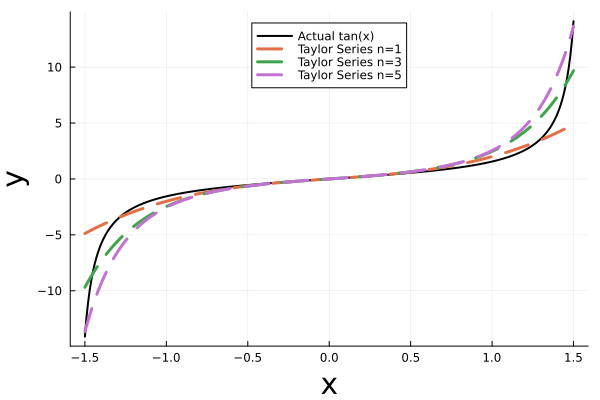
\includegraphics[width=0.6\columnwidth]{graphics/Chap05/TaylorSeriesTangent.png}%
    \caption[]{\textbf{(Taylor-Maclaurin Expansion for Tangent)} Taylor and Maclaurin studied polynomial approximations of functions based on higher-order derivatives. As such, their work extends the notion of a function's linearization, which only uses the first derivative. Because of Taylor series, people often say ``\textcolor{blue}{\bf first-order Taylor approximation}'' when they really mean the ``\textcolor{blue}{\bf linearization of a function}''. Hey, it is what it is!}
    \label{fig:TaylorSeriesTangent}
\end{figure}

 \subsection{Higher-order Derivatives Lead to Taylor's and Maclaurin's Expansions}

  In Chapter~\ref{sec:LocalLinearApproxFunction}, we showed how the notion of a linear approximation to a function near a point and the derivative of the function at that same point go hand in hand; they are really two sides of the same coin. As hinted at in Fig.~\ref{fig:TaylorSeriesTangent}, why stop at a linear approximation of a function? Why not use higher-order derivatives to propose a \href{https://en.wikipedia.org/wiki/Taylor_series}{polynomial approximation} that may be able to provide better accuracy? Progress on this question began 700 years ago by the Indian mathematician, Madhava of Sangamagrama, and then accelerated under ``the relatively more recent'' investigation by Issac Newton in the mid to late 1600's. The general theory came together under Brook Taylor in 1715. The importance of Taylor's work became more clear when Colin Maclaurin used it to characterize maxima, minima, and inflection points of functions in 1725. Today, the uses of Taylor approximations range from the creation of faster and more accurate numerical integration routines to highly efficient \href{https://developer.nvidia.com/rtx/ray-tracing}{ray tracing} algorithms that render photo-realistic images in video games. 

  \subsubsection{Fundamental Idea}

 We start with a very simple proposition that lays bare the essence of Taylor series.
 \bigskip


 \begin{propColor}{Local Polynomial Approximation}{FoundationTaylorTheorm} Consider a function\( f:(a, b) \to \real \) that is $n$-times differentiable at $0 \in (a, b)$, the origin. Then the polynomial
\begin{equation}
    p(x):=a_n \frac{x^n}{n!} + a_{n-1} \frac{x^{(n-1)}}{(n-1)!} +\cdots + a_2 \frac{x^2}{2!} + a_1 x + a_0 
\end{equation}
matches the values of $f$ and its first $n$ derivatives at the origin if, and only if, 
\begin{equation}
    a_k = f^{(k)}(0) =\frac{d^k f(x)}{dx^k} \Big|_{x=0}.
\end{equation}

\bigskip

\textbf{Note:} We have added factorial terms to the monomials. This is because 
  $$ \frac{d}{dx} \left( \frac{x^k}{k !} \right) = \frac{x^{k-1}}{(k-1) !}, \quad \frac{d^2}{dx^2} \left( \frac{x^k}{k !} \right) = \frac{x^{k-2}}{(k-2) !},\quad \frac{d^3}{dx^3} \left(\frac{x^k}{k !}  \right)=\frac{x^{k-3}}{(k-3) !}, ~~\text{etc}.$$ 

  \bigskip

\textbf{Note 2:} A similar result holds for 
$$q(x):= \sum_{k=0}^n a_k\frac{(x-x_0)^k}{k !} = a_n \frac{(x-x_0)^n}{n!} + \cdots + a_2 \frac{(x-x_0)^2}{2!} + a_1 (x-x_0) + a_0, $$
that is, $p(x)$ shifted by $x_0$. Then we need $a_k = f^{(k)}(x_0)$.
     
 \end{propColor}
 \textbf{Proof:} It is super informative to look at the second-order case first. We are interested in constructing a polynomial
\[
p(x) = a_2 \frac{x^2}{2!} + a_1 x + a_0
\]
that matches the function \(f\) and its first two derivatives at the origin.

\textbf{Function Value at the Origin:} For the polynomial \(p(x)\) to match the value of \(f(x)\) at \(x=0\), we must have
\[
p(0) = a_0 = f(0).
\]
This establishes that the constant term \(a_0\) is equal to \(f(0)\), the value of the function at the origin.

\textbf{First Derivative:} The first derivative of \(p(x)\) is
\[
p'(x) = 2a_2 \frac{x}{2!} + a_1 = \bm{a_2 x + a_1}.
\]
Matching the first derivative of \(p(x)\) with that of \(f(x)\) at \(x=0\) yields
\[
p'(0) = a_1 = f'(0).
\]
This shows that the coefficient \(a_1\) is determined by the first derivative of \(f\) at the origin.

\textbf{Second Derivative:} The second derivative of \(p(x)\) is
\[
p''(x) = a_2.
\]
Matching the second derivative of \(p(x)\) with that of \(f(x)\) at \(x=0\) gives
\[
p''(0) = a_2 = f''(0).
\]
This confirms that the coefficient \(a_2\) is equal to the second derivative of \(f\) at the origin. \\

\textcolor{blue}{\bf (Optional Read) Proof by Induction:} \textbf{Base Case:} For \(k=0\), we have \(p(0) = f(0)\), which implies \(a_0 = f(0)\). This is because all other terms in \(p(x)\) contain \(x\) and therefore vanish at \(x=0\).

\textbf{Induction Hypothesis:}  Assume that for some \(k \geq 0\), the \(k\)th derivative of \(p(x)\) equals
\[
p^{(k)}(x) = a_k + a_{k+1} \frac{x}{1!} + a_{k+2} \frac{x^2}{2!} + \cdots + a_n \frac{x^{n-k}}{(n-k)!},
\]
and that it matches the \(k\)th derivative of \(f(x)\) at \(0\), i.e.,
\[
p^{(k)}(0) = f^{(k)}(0) = a_k.
\]

\textbf{Inductive Step:} We must show that if the hypothesis holds for \(k\), it also holds for \(k+1\). Consider the \((k+1)\)st derivative of \(p(x)\):
\[
p^{(k+1)}(x) = a_{k+1} + a_{k+2} \frac{x}{1!} + \cdots + a_n \frac{x^{n-(k+1)}}{(n-(k+1))!}.
\]
Evaluating this at \(x=0\) gives
\[
p^{(k+1)}(0) = a_{k+1},
\]
which, by the definition of \(p(x)\), must equal \(f^{(k+1)}(0)\). Therefore, for the polynomial \(p(x)\) to match \(f\) and its first \(n\) derivatives at \(0\), we have
\[
a_{k+1} = f^{(k+1)}(0):=\frac{d^{k+1} f(x)}{dx^{k+1}} \Big|_{x=0}.
\]

By the principle of mathematical induction, this completes the proof, showing that each coefficient \(a_k\) of the polynomial \(p(x)\) must be chosen as \(a_k = f^{(k)}(0)\) for the polynomial to match \(f\) and its first \(n\) derivatives at the origin.


 \Qed

 \subsubsection{The Actual Taylor and Maclaurin Polynomials}



\vspace*{.2cm}

\begin{tcolorbox}[colback=mylightblue, title = {\bf Taylor and Maclaurin Polynomials}, breakable]
Let \( f:(a, b) \to \real \) be a function defined on an open interval $(a, b)$ and let $x_0 \in (a, b)$. Recall that if $f$ is once differentiable at $x_0$, then 
 $$ f(x) \approx f(x_0) + \frac{ df(x_0)}{dx} \cdot (x - x_0) ~~\text{or with the prime notation}~~f(x) \approx  f(x_0) + f'(x_0) \cdot (x - x_0) $$
is the \textbf{linear approximation} of the function about $x_0$.\\

\begin{definition} 
\label{def:TaylorPolynomial}
Suppose that \( f:(a, b) \to \real \) is $n$-times differentiable at $x_0$. Then
\begin{equation}
f(x) \approx f(x_0) + f'(x_0)(x-x_0) + f''(x_0)\cdot \frac{(x-x_0)^2}{2!} + \cdots + f^{(n)}(x_0)\frac{(x-x_0)^n}{n!},
\end{equation}
is the \textbf{$\bm{n}$-th degree Taylor expansion of $\bm{f}$ about the point $\bm{x_0}$}. For the special case $x_0=0$ (the origin), 
\begin{equation}
f(x) \approx f(0) + f'(0)\cdot x + f''(0)\cdot \frac{x^2}{2!} + \cdots + f^{(n)}(0)\cdot \frac{x^n}{n!} 
\end{equation}
is called an \textbf{$\bm{n}$-th degree Maclaurin polynomial or Maclaurin expansion}.
\end{definition}

\bigskip

\textbf{Note:} The Taylor expansion is the unique polynomial of degree $n$ that exactly matches the values of $f$ and its first $n$ derivatives at the point $x_0$.\\

\textbf{Note 2:} There is a nice theory for quantifying the approximation error when using a Taylor expansion. Here is a very clear \href{https://www.dropbox.com/scl/fi/n9of97gbhtll4rgy5l005/Estimation-of-the-Taylor-Remainder.pdf?rlkey=xyzk8aiuroo6wjl2aiqbzbbyf&dl=0}{written document} by the University of South Carolina and here is a \href{https://www.youtube.com/watch?v=lY0LzJXTgeo}{video} by the Organic Chemistry Tutor.
\end{tcolorbox}

\vspace*{.2cm}


\subsubsection{Taking it to the Limit}

Many functions can be differentiated an infinite number of times. For example, $e^x$ is \textbf{infinitely differentiable} because $\frac{d}{dx} e^x = e^x$ implies that  $\frac{d^k}{dx^k} e^x = e^x$ for all $k\ge 1$. Sine and cosine are also infinitely differentiable because of the simple chain of derivatives,
$$\frac{d}{dx} \sin(x) = \cos(x) \quad \text{and} \quad \frac{d}{dx} \cos(x) = -\sin(x).  $$
In fact, the \(k\)-th derivative of \(\sin(x)\) is
\[
\frac{d^k}{dx^k} \sin(x) = 
\begin{cases} 
~~~ \sin(x) & \text{if } k \equiv 0 \pmod{4} \\
~~~ \cos(x) & \text{if } k \equiv 1 \pmod{4} \\
-\sin(x) & \text{if } k \equiv 2 \pmod{4} \\
-\cos(x) & \text{if } k \equiv 3 \pmod{4}
\end{cases}
\]
and the \(k\)-th derivative of \(\cos(x)\) is
\[
\frac{d^k}{dx^k} \cos(x) = 
\begin{cases} 
~~~ \cos(x) & \text{if } k \equiv 0 \pmod{4} \\
-\sin(x) & \text{if } k \equiv 1 \pmod{4} \\
-\cos(x) & \text{if } k \equiv 2 \pmod{4} \\
~~~ \sin(x) & \text{if } k \equiv 3 \pmod{4}.
\end{cases}
\]
For functions that are infinitely differentiable, one can propose an \textbf{infinite} Taylor or Maclaurin series representation of the function.  \\

\begin{factColor}{(Infinite) Taylor Series Expansion}{TaylorSeries}

The Taylor series expansion of an infinitely differentiable function $f(x)$ around a point $x_0$ is given by,
\begin{equation}
    f(x) = f(x_0) + f'(x_0)(x-x_0) + \frac{f''(x_0)}{2!}(x-x_0)^2 + \frac{f'''(x_0)}{3!}(x-x_0)^3 + \cdots = \lim_{n \to \infty} \sum_{k=0}^{n} \frac{f^{(k)}(x_0)}{k!}(x-x_0)^k,
\end{equation}
where $f^{(k)}(x_0)$ denotes the $k$-th derivative of $f$ evaluated at the point $x_0$. \\

Whether or not the limit in an infinite Taylor series converges is a highly technical question that we will not explore. Nevertheless, there are three CONVERGENT infinite Maclaurin series that show up frequently in Engineering and STEM. We highlight them below:\\

\textbf{Expansion for $e^x$}
\begin{equation}
\label{eq:taylorSeriesNaturalExponetial}
    e^x = 1 + x + \frac{x^2}{2!} + \frac{x^3}{3!} + \cdots = \lim_{n \to \infty} \sum_{k=0}^{n}  \frac{x^k}{k!},
\end{equation}

\textbf{Expansion for $\sin(x)$}
\begin{equation}
    \sin(x) = x - \frac{x^3}{3!} + \frac{x^5}{5!} - \frac{x^7}{7!} + \cdots = \lim_{n \to \infty} \sum_{k=0}^{n}  \frac{(-1)^k x^{2k+1}}{(2k+1)!},
\end{equation}

\textbf{Expansion for $\cos(x)$}
\begin{equation}
    \cos(x) = 1 - \frac{x^2}{2!} + \frac{x^4}{4!} - \frac{x^6}{6!} + \cdots = \lim_{n \to \infty} \sum_{k=0}^{n}  \frac{(-1)^k x^{2k}}{(2k)!}.
\end{equation}

If we were to add a fourth one, it would be the expansion for $\ln(1 + x)$.
    
\end{factColor}

\subsubsection{Deriving Euler's Formula from Fact~\ref{thm:TaylorSeries}}

Euler's formula, $e^{\im x} = \cos(x) + \im \sin(x)$, follows from the three Taylor series in Fact~\ref{thm:TaylorSeries}. Here is how it goes. We first DEFINE $e^{\im x}$ by substituting \(\im x\) for \(x\) into \eqref{eq:taylorSeriesNaturalExponetial}. Yes, otherwise, we do not know how to evaluate the function with a complex argument. However, we know how to perform algebra on terms like $(\im x)^k$. \\

\textcolor{blue}{\bf This approach to defining $\bm{e^{\im x}}$ through a power series is in and of itself a powerful use of Taylor series}; continuing, we have 
\[
e^{\im x} := 1 + \im x + \frac{(\im x)^2}{2!} + \frac{(\im x)^3}{3!} + \frac{(\im x)^4}{4!} + \cdots
\]
Then, because $\im^k = \begin{cases}
    ~~1 & k = 0~~{\rm mod}~~ 4\\
   ~~\im & k = 1~~{\rm mod} ~~4\\
   -1 & k = 2~~{\rm mod} ~~4\\
   -\im & k = 3~~{\rm mod}~~ 4,\\
\end{cases}$
the above simplifies to,
\[
e^{\im x} = 1 + \im x - \frac{x^2}{2!} - \im \frac{x^3}{3!} + \frac{x^4}{4!} + \im \frac{x^5}{5!} \cdots
\]

Grouping the real and imaginary parts, yields
\[
e^{\im x} = \left(1 - \frac{x^2}{2!} + \frac{x^4}{4!} - \cdots\right) + \im \left(x - \frac{x^3}{3!} + \frac{x^5}{5!} - \cdots\right)
\]

The series within the parentheses are recognized as the Taylor series expansions of \(\cos(x)\) and \(\sin(x)\), respectively,
\[
\cos(x) = 1 - \frac{x^2}{2!} + \frac{x^4}{4!} - \cdots
\]
\[
\sin(x) = x - \frac{x^3}{3!} + \frac{x^5}{5!} - \cdots
\]

Therefore, by direct comparison, we obtain
\[
e^{\im x} = \cos(x) + \im \sin(x).
\]
\Qed

\subsubsection{Don't Fall for the Hype}

 Thanks to ROB 101 \textit{Computational Linear Algebra}, you know how to fit polynomials to functions. You also know how to build approximations with radial basis functions. For many applications, these sorts of approximations are superior to Taylor expansions. Taylor expansions are one tool among many in your algorithmic toolbox. \\

 \begin{funColor}{Taylor Series are often Over Hyped}{TaylorSeriesSlam}
 When the pinnacle of calculus applications you have to offer a student is the Taylor series, consider yourself in dire straits. This blunt truth cuts through the academic grandeur that has elevated the Taylor series to a pedestal for over seven decades. Despite its theoretical elegance, the harsh reality is that, beyond the realm of first-order linearizations, Taylor series rarely grace the practical world of engineering. This stark contrast exposes a glaring discrepancy between traditional calculus education and the actual demands of engineering practice. The hyping of Taylor series as a major application of Calculus not only misleads but also underprepares students for the challenges they will face in applying Calculus creatively outside the classroom. In essence, if the Taylor series is your go-to case study for the wonders of Calculus, you're not just propagating an untruth; you're supporting a profound educational failure that has persisted for far too long.
 \end{funColor}

\subsubsection{For Further Learning}
\begin{itemize}
\item \href{https://youtu.be/BLkz5LGWihw}{Higher order derivatives} by \threebb.

    \item \href{https://youtu.be/3d6DsjIBzJ4}{Taylor series}  by \threebb.

    \item \href{https://www.youtube.com/watch?v=epgwuzzDHsQ}{Taylor \& Maclaurin Polynomials: Intro} Khan Academy.

    \item \href{https://www.youtube.com/watch?v=ebfOSDj4j3I}{Taylor Series and Power Series Made Easy (with Pictures): Review of Calculus} by Steve Brunton.

    \item \href{https://youtu.be/H0Zbg_CqMCs}{Taylor Series of the Exponential Function and Euler's Formula!} by Steve Brunton.
\end{itemize}



\begin{table}[ht]
\centering
\begin{tabular}{|c|c|c|}
\hline
\( m \) & Expression for \( {\rm Im} \left\{  (1 + i)^m\right\} \) & Answer \\
\hline
0 & \( {\rm Im} \left\{  (1 + i)^{0}\right\} \) & 0 \\
1 & \( {\rm Im} \left\{  (1 + i)^1\right\} \) & 1 \\
2 & \( {\rm Im} \left\{  (1 + i)^2\right\} \) & 2 \\
3& \( {\rm Im} \left\{  (1 + i)^3\right\} \) & 2 \\
4 & \( {\rm Im} \left\{  (1 + i)^4\right\} \) & 0 \\
5 & \( {\rm Im} \left\{  (1 + i)^5\right\} \) & $-2^2$ \\
6& \( {\rm Im} \left\{  (1 + i)^6\right\} \) & $-2^3$\\
7& \( {\rm Im} \left\{  (1 + i)^7\right\} \) & $-2^3$ \\
\hline
\end{tabular}
\caption{A Y2K generalization can be found in this table of values for \( m \), expressions for \( {\rm Im} \left\{  (1 + i)^m\right\} \), and computed numbers.}
\end{table}

\subsection {(Optional Read:) Y2K or \bprp~ Strikes Again}

While the original \href{https://en.wikipedia.org/wiki/Year_2000_problem}{Y2K Problem} was of potential major significance for our engineered world, the following problem has zero engineering relevance. Nevertheless, many of us got into engineering because we liked math. Hence, scratching that itch is a worthwhile endeavor. \\

\textbf{Problem:} Compute $ \left. \frac{d^{2000}}{dx^{2000}}\left( e^x \cdot \sin(x) \right) \right|_{x=0}.$ Yes, the Y2K derivative of $e^x \cdot \sin(x)$ evaluated at the origin. \\

\Ans ~~1~BCE\footnote{The year immediately before 1 CE (Common Era) is 1 BCE (Before Common Era). There is no year 0 in the Gregorian calendar system, so it jumps directly from 1 BCE to 1 CE. Does this mean that 1 BCE, being the year before 1 CE, functions as zero?.}.\\

\textbf{Why:} Recall Euler's formula: $e^{\im x} = \cos(x) + \im \sin(x)$. Hence, we can write
$$ \sin(x) = {\rm Im} \{ e^{\im x} \},$$
where ${\rm Im}$ stands for the imaginary part. Our problem can, therefore, be written as 
$$ \left. \frac{d^{2000}}{dx^{2000}}\left( {\rm Im} \{e^x \cdot e^{\im x} \} \right) \right|_{x=0} =  
\left. {\rm Im} \left\{\frac{d^{2000}}{dx^{2000}}\left( e^x \cdot e^{\im x}  \right) \right|_{x=0}\right\} = \left. {\rm Im} \left\{\frac{d^{2000}}{dx^{2000}}\left(e^{(1 + \im)  x}  \right) \right|_{x=0}\right\}. $$

This greatly simplifies things because 
$$\left. \frac{d^k}{dx^k}\left( e^{\alpha x} \right) \right|_{x=0} = \left. \alpha^k \cdot e^{\alpha x} \right|_{x=0} = \alpha^k,$$
even for $\alpha \in \cp$.
It follows that, 
$$ \left. \frac{d^{2000}}{dx^{2000}}\left( e^x \cdot \sin(x) \right) \right|_{x=0}  =   {\rm Im}\{ (1 + \im)^{2000} \},$$
and while this may look painful, it is not! We first note that 
$$(1+ \im)^2 = (1 + 2 \im +(\im)^2)) = (1 + 2 \im -1) = 2\im. $$
Then, we note that 
$$(1+ \im)^8 = ( 2\im)^4 = 2^4, $$
because $\im^4 = (-1)^2 = 1.$ Do you see where this is going? $2000 = 8 \cdot 250.$
Hence, using our exponent rules, 
$$ (1 + \im)^{2000} = \left( (1 + \im)^{8} \right)^{250} = \left( 2^4 \right)^{250} = 2^{1000},$$
a real number. We conclude that 
$$\left. \frac{d^{\rm Y2K}}{dx^{\rm Y2K}}\left( e^x \cdot \sin(x) \right) \right|_{x=0} = \left. \frac{d^{2000}}{dx^{2000}}\left( e^x \cdot \sin(x) \right) \right|_{x=0} = {\rm Im} \left\{ (1 + \im)^{2000} \right\} = {\rm Im} \left\{ 2^{1000}\right\} = 0.$$

Here's the link to \bprp's \href{https://youtu.be/xu5elUhRg4E?t=190}{video} solving the tiebreaker problems from the 2022 Berkeley Math Tournament. The Berkeley version of the problem is ever so slightly different. After watching the video, can you generalize the problem to 
$$\text{\bf Find:}~~ \left. \frac{d^{\rm Year}}{dx^{\rm Year}}\left( e^x \cdot \sin(x) \right) \right|_{x=0}?$$

\textbf{Hint:} Given in the footnote\footnote{Write ${\rm Year} = 8 \cdot N + m$, where $m \in \{0, 1, 2, \ldots, 7\}$. Then the answer is $2^{4 \cdot N} \cdot {\rm Im} \left\{ (1 +\im)^m \right\}$. You are almost there.} so that you can play with the problem first. Scratch that itch!

%%%%%%%%%%%%%
\section{Partial Derivatives}


Because you have taken Linear Algebra already, where you solved problems involving thousands of variables, working with functions of a single variable must seem somewhat ``tame''. The training of modern AI Neural Networks involves literally billions of variables where their derivatives are computed via Automatic Differentiation (AD); see Chapter~\ref{sec:AutomaticDifferentiation}. While we will NOT attempt any examples of this magnitude (look for a course on Deep Learning), we will treat \textbf{multivariable (aka, multivariate)} functions in \(n>1\) variables. It is suggested that you review Chapter 11.5 in the ROB 101 \textit{Computational Linear Algebra} \href{https://grizzle.robotics.umich.edu/education/rob101.html}{textbook}.

\subsection{Intuition}

Imagine you're standing somewhere on the side of a mountain, and you want to know how fast you're ascending or descending. You can use partial derivatives to figure this out. Partial derivatives are a way of measuring how a function changes when one of its inputs changes while keeping all of the other inputs the same. Since you're standing on a mountain, let's take the function as your altitude (aka, height) and the inputs as your \((x, y)\) position on the mountain.

If you compute the local slope of your function as \(x\) varies while holding \(y\) constant, it is called a \textbf{partial derivative with respect to \(\bm{x}\)}. \textcolor{blue}{\bf Why partial?} Because you are only considering a ``small part of the variables'' (one at a time) and not ``all of them'' (together). The partial derivative with respect to \(x\) would tell you the rate of change of your altitude as you move a small amount in an eastward direction (i.e., move to the right), \textcolor{blue}{\bf while keeping \(y\) constant}. A partial derivative with respect to \(y\) would tell you the rate of change of your altitude as you move a small amount northward (i.e., straight ahead), \textcolor{blue}{\bf while keeping \(x\) constant}. It is the ``slope'' or rate of change taken one variable at a time, a kind of divide and conquer approach. Don't worry; we can still obtain information on the ``slope'' when all variables are considered.

\textbf{A partial derivative is a little like how a basis for vectors allows you to understand how much each individual basis vector contributes to a given vector, and by adding up all of the contributions, you can reconstruct the entire vector}. Recall, if
\[
\{u_1, u_2, \ldots, u_n\}
\]
is a basis for \(\mathbb{R}^{n}\), then we can write any vector \(v \in \mathbb{R}^{n}\) as a linear combination of the basis vectors, that is,
\[
v = \alpha_1 u_1 + \alpha_2 u_2 + \cdots + \alpha_n u_n.
\]
The quantity \(\bm \alpha_i \bm u_i\) is the \textbf{component of \(\bm v\)} lying in the \textbf{direction \(\bm u_i\)}.

We will see that partial derivatives are EXACTLY LIKE THIS, and in the best possible way. \textbf{How's that? Best possible way!} We use the natural basis vectors, \(\{e_1, e_2, \ldots, e_n\}\), to define partial derivatives. For definiteness, we recall that in \(\mathbb{R}^{n}\), the \textbf{natural basis vectors (aka, canonical basis vectors)} are the columns of the \(n \times n\) identity matrix, that is,
\[
e_1:= \left[ \begin{array}{c} 1 \\ 0 \\ 0 \\ \vdots \\ 0 \end{array}\right], ~e_2:= \left[ \begin{array}{c} 0 \\ 1 \\ 0 \\ \vdots \\ 0 \end{array}\right], ~e_3:= \left[ \begin{array}{c} 0 \\ 0 \\ 1 \\ \vdots \\ 0 \end{array}\right], \ldots, ~e_n:= \left[ \begin{array}{c} 0 \\ 0 \\ 0 \\ \vdots \\ 1 \end{array}\right]
\]

\subsection{Partial Derivatives: Single-variable Derivatives meet Multivariable Functions}
\label{sec:PartialDerivatives}

To set the stage, let's note that if \(f:\mathbb{R}^{n} \to \mathbb{R}^{m}\) is a vector-valued function depending on \(x=(x_1, x_2, \ldots, x_n)\), \(x_0 \in \mathbb{R}^{n}\), and \(h \in \mathbb{R}\), then \(g(h):= f(x_0 + h \cdot e_i)\) if only a function of \(h\); it is a single-variable function. As an example, consider
\[
f(x_1, x_2) := \left[ \begin{array}{c} x_1 \cdot x_2 \\ e^{x_1} + \sin(x_2) \end{array}\right]
\]
and let \(x_0= (3, \frac{\pi}{4})\). Then
\[
g(h):= f(x_0 + h \cdot e_1) = f\left( \left[ \begin{array}{c} 3 \\ \frac{\pi}{4} \end{array}\right] + h\cdot \left[ \begin{array}{c} 1 \\ 0 \end{array}\right]\right) =f(3+h, \frac{\pi}{4}) = \left[ \begin{array}{c} (3 + h) \cdot \frac{\pi}{4}\\ e^{3 + h} + \sin\left(\frac{\pi}{4}\right) \end{array}\right],
\]
and
\[
\gamma(h):= f(x_0 + h \cdot e_2) = f\left( \left[ \begin{array}{c} 3 \\ \frac{\pi}{4} \end{array}\right] + h\cdot \left[ \begin{array}{c} 0 \\ 1 \end{array}\right]\right) = f(3, \frac{\pi}{4} +h) = \left[ \begin{array}{c} 3 \cdot \left( \frac{\pi}{4} +h \right) \\ e^{3} + \sin\left(\frac{\pi}{4} +h\right) \end{array}\right].
\]

Each of these functions depends on \(h\) alone. And where \(h\) shows up in the function is dictated by which basis vector \(e_i\) is used in forming \(f(x_0 + h \cdot e_i)\). The first function depends on \(h\) everywhere that \(f\) depends on \(x_1\), and the second function depends on \(h\) everywhere that \(f\) depends on \(x_2\). Once again, this is a divide-and-conquer strategy that works very well. Moreover, because these functions depend on a single variable, we can use our limit concept from Def.~\ref{def:derivAtPoint} to define a partial derivative! \textbf{Yes, partial derivatives are ``rise over run'' computed one variable at a time}.

\begin{tcolorbox}[colback=mylightblue, title = {\bf Partial Derivative at a Point}, breakable]

\begin{definition}
\label{def:partialDerivAtPoint}
Suppose \(f:\mathbb{R}^{n} \to \mathbb{R}^{m}\) is a vector-valued function depending on \(x=(x_1, x_2, \ldots, x_n)\) and that \(x_0 \in \mathbb{R}^{n}\) is a point (aka, a fixed vector). The \textbf{partial derivative of \(\bm{f}\) with respect to \(\bm{x_i}\) at the point \(\bm{x_0}\)} is
\begin{equation}
\label{eq:partialDerivAtPoint}
\begin{aligned}
\frac{\partial f(x_0)}{\partial x_i} :=& \lim_{h \to 0} \frac{f(x_0 + h\cdot e_i) - f(x_0)}{h} \\
\frac{\partial f(x_0)}{\partial \bm{x_i}} :=&  \lim_{h \to 0} \frac{f(x_0 + h\cdot \bm{e_i}) - f(x_0)}{h}~~(\text{same as above, highlighting}~ \bm{x_i} \text{ and } \bm{e_i}),
\end{aligned}
\end{equation}
assuming the limit exists and is finite.

\textbf{Notes:}
\begin{itemize}
\item  To distinguish a ``partial'' derivative from an ``ordinary'' derivative, we replace \(d\) with the symbol \(\partial\), which is pronounced, ``partial''.
\item The symbol \(\frac{\partial f(x_0)}{\partial x_i}\) is called the ``partial derivative of \(f\) with respect to \(x_i\), evaluated at \(x_0\). Yeah, that's a mouthful. That's why math symbols are useful. A few of them can stand for a ton of words as we saw in Chapter~\ref{sec:GoodNotationDescartes}, when we discussed Descartes vs. the Babylonians.
\item Because the function \(f:\mathbb{R}^{n} \to \mathbb{R}^{m}\) has \(m\)-components, that is,
\[
f(x_1, x_2, \ldots, x_n) = \left[ \begin{array}{c} f_1(x_1, x_2, \ldots, x_n) \\ f_2(x_1, x_2, \ldots, x_n) \\ \vdots \\ f_m(x_1, x_2, \ldots, x_n) \end{array}\right],
\]
\textcolor{blue}{\bf \large the limit in \eqref{eq:partialDerivAtPoint} must exist and be finite for} \textcolor{black}{\bf \large each component of the function, that is, for each \(\bm {f_i(x_1, x_2, \ldots, x_n)}\), or the partial derivative does not exist.}
\end{itemize}

\end{definition}
\end{tcolorbox}

\begin{center}
\setlength{\fboxrule}{2pt}  % Setting the thickness of the border line
   \fbox{ \parbox{0.9\linewidth}{\textcolor{blue}{\bf Didn't we just stop using limits to compute the derivative with respect to a single variable?} \textcolor{red}{\bf  Yes!} We compute partial derivatives the same way as ordinary derivatives because we are only differentiating with respect to one variable at a time, as in
 $$\mathlarger{\frac{\partial f(x_0)}{\partial \bm{x_i}} = \left. \frac{d}{dh} f(x_0 + h \cdot \bm{e_i}) \right|_{h = 0}},$$
 and hence, all of the rules in Prop.~\ref{thm:DifferentiationRules} for ordinary derivatives apply to partial derivatives as well. Moreover, we have Software tools for turning gnarly problems into manageable problems. We illustrate all of this next. }
}
\end{center}

\begin{example}
Compute--by hand--the partial derivatives of
\[
f(x_1, x_2) := \left[ \begin{array}{c} x_1 \cdot x_2 \\ e^{x_1} + \sin(x_2) \end{array}\right]
\]
at a general point, \(x \in \mathbb{R}^2\). In other words, you do not have to evaluate them at a specific point.
\end{example}

\textbf{Solution:}
\[
\frac{\partial}{\partial x_1} f(x_1, x_2) = \frac{\partial}{\partial x_1} \left[ \begin{array}{c} x_1 \cdot x_2 \\ e^{x_1} + \sin(x_2) \end{array}\right] = \left[ \begin{array}{l} \frac{\partial}{\partial x_1}( x_1 \cdot x_2) \\ \frac{\partial}{\partial x_1}(e^{x_1} + \sin(x_2)) \end{array}\right]= \left[ \begin{array}{c} x_2 \\ e^{x_1}\end{array}\right].
\]
Indeed, when taking the derivative with respect to \(x_1\), we treat everything else as a constant,
\begin{itemize}
\item \(\frac{\partial}{\partial x_1}(x_1 \cdot x_2) = x_2\) (we think of \(x_2=c\), a constant),
\item \(\frac{\partial}{\partial x_1}(\sin(x_2)) = 0\) (we think of \(x_2=c\), a constant), and
\item \(\frac{\partial}{\partial x_1}(e^{x_1}) = e^{x_1}\) (because the derivative of \(e^{x_1}\) is itself).
\end{itemize}

Next,
\[
\frac{\partial}{\partial x_2} f(x_1, x_2) = \frac{\partial}{\partial x_2} \left[ \begin{array}{c} x_1 \cdot x_2 \\ e^{x_1} + \sin(x_2) \end{array}\right] =\left[ \begin{array}{l} \frac{\partial}{\partial x_2}( x_1 \cdot x_2) \\ \frac{\partial}{\partial x_2}(e^{x_1} + \sin(x_2)) \end{array}\right]= \left[ \begin{array}{c} x_1 \\ \cos(x_2)\end{array}\right].
\]
Indeed, when taking the derivative with respect to \(x_2\), we treat everything else as a constant,
\begin{itemize}
\item \(\frac{\partial}{\partial x_2}(x_1 \cdot x_2) = x_1\) (we think of \(x_1=c\), a constant),
\item \(\frac{\partial}{\partial x_2}(e^{x_1}) = 0\) (we think of \(x_1=c\), a constant), and
\item \(\frac{\partial}{\partial x_2}(\sin(x_2)) = \cos(x_2)\) (because the derivative of \(\sin(x_2)\) is \(\cos(x_2)\)).
\end{itemize}

\Qed

\begin{rem} Why do we sometimes write  \(\frac{\partial f(x_1, x_2)}{\partial x_1}\) and sometimes \(\frac{\partial}{\partial x_1} f(x_1, x_2)\)? Because
$$\frac{\partial}{\partial x_1} \left[ \begin{array}{c} x_1 \cdot x_2 \\ e^{x_1} + \sin(x_2) \end{array}\right]
\text{\bf looks much better than} \frac{\partial \left[ \begin{array}{c} x_1 \cdot x_2 \\ e^{x_1} + \sin(x_2) \end{array}\right]}{ \partial x_1}.$$       
Don't you agree? Also, it's good to recognize differentiation as an operator that is applied to functions.
\Qed
\end{rem}

%%%%%%%%%%

\section{Packaging Partial Derivatives to form Jacobians, Gradients, and Hessians}
\label{sec:PackagingPartialDerivatives}

Jacobians and gradients are matrix and vector forms, respectively, of partial derivatives. They collect all of the ``local slope information'' into a single object, just as we learned to do for linear equations, $A x = b$. The Hessian is the Jacobian of the gradient. Much of this material is based on Chapter 11.5 of the ROB 101 \textit{Computational Linear Algebra} 
\href{https://www.dropbox.com/s/1pzva81t4shnd22/ROB_101_Textbook_11April2023.pdf?dl=0}{textbook}. 

\subsection{The Jacobian}

Consider a multivariable vector-valued function $f:\real^{n} \to \real^{m}$. The notation introduced in Chapter~\ref{sec:PartialDerivatives} for partial derivatives allows us to make the following very compact definition.

\vspace*{.2cm}

\begin{tcolorbox}[colback=mylightblue, title = {\bf Jacobian of a Function}, breakable]

\begin{definition} 
\label{def:Jacobian}
The \textbf{Jacobian} of $f:\real^{n} \to \real^{m}$ is
\begin{equation}
    \label{eq:DefJacobian}
    \frac{\partial f(x)}{\partial x}:=  \left[\begin{array}{cccc}
      \frac{\partial f(x)}{\partial x_1} & \frac{\partial f(x)}{\partial x_2} & \cdots & \frac{\partial f(x)}{\partial x_n}
    \end{array} \right],
\end{equation}
assuming the indicated partial derivatives exist. 
The Jacobian of a function is formed by packaging the column vectors $\frac{\partial f(x)}{\partial x_j}$ into a matrix. We need to keep in mind that, for each value of $x\in \real^{n}$, the compact and innocent-looking object
$$ \frac{\partial f(x)}{\partial x} $$
is really an $m \times n$ matrix: because there are $n$ columns of the form $ \frac{\partial f(x)}{\partial x_j}$, and each column is an $m$-vector. There are software tools that compute the Jacobian in one fell swoop. \\

\textbf{Note:} The Jacobian of a function has two common notations (i) $\frac{\partial f(x)}{\partial x}$ as we used above, and (ii) $J_f(x)$. 

\end{definition}
\end{tcolorbox}

 \vspace*{.2cm}

Just for the record, we write out $\frac{\partial f(x)}{\partial x}$ as an $m \times n$ matrix. Suppose
$$f(x) = \left[
\begin{array}{c}
f_1(x) \\
f_2(x)\\
\vdots \\
f_m(x)\\
\end{array}
\right] =  \left[ \begin{array}{c}
f_1(x_1, x_2, \dots, x_n) \\
f_2(x_1, x_2, \dots, x_n)\\
\vdots \\
f_m(x_1, x_2, \dots, x_n)\\
\end{array}
\right].$$
Writing out all of the entries in the $m \times n$ Jacobian matrix gives 
\begin{equation}
    \label{eq:VectorFunctions03}
    \frac{\partial f(x)}{\partial x} := \left[\begin{array}{cccc}
      \frac{\partial f(x)}{\partial x_1} & \frac{\partial f(x)}{\partial x_2} & \cdots & \frac{\partial f(x)}{\partial x_n}
    \end{array} \right] =\left[\begin{array}{cccc}
      \frac{\partial f_1(x)}{\partial x_1} & \frac{\partial f_1(x)}{\partial x_2} & \cdots & \frac{\partial f_1(x)}{\partial x_n} \medskip \\
      \frac{\partial f_2(x)}{\partial x_1} & \frac{\partial f_2(x)}{\partial x_2} & \cdots & \frac{\partial f_2(x)}{\partial x_n} \medskip \\
      \vdots & \vdots & \ddots & \vdots \medskip \\
      \frac{\partial f_m(x)}{\partial x_1} & \frac{\partial f_m(x)}{\partial x_2} & \cdots & \frac{\partial f_m(x)}{\partial x_n} 
    \end{array} \right],
\end{equation}
which is much more intimidating than \eqref{eq:DefJacobian}. In other symbols, the $ij$ component of $J_f(x) = \frac{\partial f(x)}{\partial x}$ is
\begin{equation}
\label{eq:JacobianEachEntry}
\begin{aligned}
    \left[ \frac{\partial f(x)}{\partial x}  \right]_{ij} &= \frac{\partial f_i(x)}{\partial x_j} \\
    J_{ij}(x) & = \frac{\partial f_i(x)}{\partial x_j},
\end{aligned}
\end{equation}
\\

If you want to toss out the window all of the benefits of vector-matrix notation, you can compute each entry of the Jacobian matrix one by one, as in \eqref{eq:JacobianEachEntry}.
When doing hand computations for simple examples, such as $m=n=2$, the above very explicit $1 \times 1$ scalar (i.e., non-vectorized) calculations can be informative.

\newpage

\begin{propColor}{Linear Approximation at a Point for Multivariable Functions}{LinearApproxMultiVariable}
The linear approximation of a (nonlinear) function $f:\real^{n} \to \real^{m} $ at a point $x_0$ is defined to be
 \begin{equation}
     \label{eq:DefineVectorLinearApprox}
     f(x) \approx f(x_0) + A ( x - x_0) := f(x_0) + \frac{\partial f(x_0)}{\partial x} ( x - x_0),
 \end{equation}
 where the $m \times n$ matrix $A:=J_f(x_0)=\frac{\partial f(x_0)}{\partial x}$ is the Jacobian of $f$ at the point $x_0$. We note that the dimensions make sense because $f(x_0)$ is $m \times 1$, $( x - x_0)$ is $n \times 1$, and therefore $J_f(x_0)( x - x_0) = \frac{\partial f(x_0)}{\partial x}  ( x - x_0)$ is $(m \times n) \cdot (n \times 1) = m \times 1$.  \\

 \textbf{Note:} The linear approximation is also called the \textcolor{blue}{\bf first-order Taylor expansion of $f$ about the point $x_0$. Probably, at least 50\% of engineering uses this local linear approximation of a function.}
\end{propColor}

\vspace*{0.2cm}

\textbf{Proof:} We pose
\begin{equation}
    \label{eq:AffineMatrixApprox01}
    f(x) \approx  y_0 + A \cdot (x-x_0)
\end{equation}
for $||x-x_0|| < \delta$ and some $\delta>0$. What values should we assign to $y_0$ and $A$? Just as in the case of a scalar-valued function of a single variable, if we plug $x =x_0$ into \eqref{eq:AffineMatrixApprox01}, we obtain
$$ f(x_0) = y_0.$$
Hence, 
\begin{equation}
    \label{eq:AffineMatrixApprox02}
    f(x) \approx  f(x_0) + A\cdot(  x-x_0).
\end{equation}
Next, we plug in $x=x_0 + h\cdot e_i$ into \eqref{eq:AffineMatrixApprox02}, yielding
\begin{align*}
    f(x_0 + h\cdot e_i) &\approx  f(x_0) + \underbrace{A\cdot h\cdot e_i}_{h\cdot e_i=(x_0 + h\cdot e_i)-x_0} \\
    & \approx f(x_0) + h \cdot A \cdot e_i \\
    & \approx f(x_0) + h \cdot A_i,
\end{align*} 
where we note that $ A \cdot e_i = A_i$, the $i$-th column of $A$. A little algebra gives us
\begin{equation}
    \label{eq:AffineMatrixApprox03}
  \big(  f(x_0 + h\cdot e_i) - f(x_0) \approx h\cdot A_i \big) \iff \left( A_i \approx  \frac{ f(x_0 + h\cdot e_i) - f(x_0) }{h} \right).
\end{equation}
The approximation should be better and better with smaller and smaller $h$. In the limit, we have
\begin{equation}
    \label{eq:AffineMatrixApprox04}
A_i= \lim_{h \to 0} \frac{ f(x_0 + h\cdot e_i) - f(x_0) }{h}=: \frac{\partial f(x_0)}{\partial x_i},
\end{equation}
as long as the limit exists. In other symbols, if $f$ is differentiable at $x_0$, once we assemble the columns of 
$$A=  \left[\begin{array}{cccc}
      \frac{\partial f(x_0)}{\partial x_1} & \frac{\partial f(x_0)}{\partial x_2} & \cdots & \frac{\partial f(x_0)}{\partial x_n}
    \end{array} \right],$$ 
we have
\begin{equation}
    \label{eq:AffineMatrixApprox05}
    f(x) \approx  f(x_0) +  \frac{\partial (x_0)}{ \partial x} \cdot (x-x_0)
\end{equation}
is a \textbf{local linear approximation} to the function near the point $x_0$.

\Qed

\begin{funColor}{Use of First-Order Taylor Expansions in Engineering}{LinearApproxVectorFunctions}

    The use of \textbf{first-order Taylor expansions}, often referred to as \textbf{linear approximations}, is pervasive in various fields of engineering. While it's difficult to quantify ``how much'' of engineering is based on this concept, it's safe to say that it's a fundamental tool used frequently for analysis, design, and optimization. Here are some areas where it's commonly used:\\

\textbf{Feedback Control Systems:} In control theory, nonlinear systems are often linearized around an operating point to make them easier to analyze and control. The linearized models are then used to design controllers. {\bf We will make use of linearization when we design feedback controllers for the Ball Bot.} A cool thing about the use of linearizations in feedback control is that \textbf{the controller is trying to keep an error term small}, and this error is often $(x-x_0)$. In other words, the controller is helping to validate the assumptions required for using a linear approximation in the first place. \\

\textbf{Structural Engineering:} In the analysis of structures like beams, bridges, and buildings, linear approximations are often used to simplify complex equations describing deformation and stress. \\

\textbf{Electrical Engineering:}
In circuit analysis, devices like transistors are often modeled using linear approximations around an operating point, especially for small-signal analysis. \\

\textbf{Fluid Mechanics:}
In fluid dynamics, linear approximations are used to simplify the Navier-Stokes equations under certain conditions, leading to more tractable models like potential flow. \\

\textbf{Thermodynamics:}
In thermodynamics, properties like enthalpy and entropy are often linearized to analyze processes like isothermal and adiabatic expansions. \\

\textbf{Signal Processing:}
In signal processing, systems are often linearized to make them easier to analyze using Fourier and Laplace transforms. \\

\textbf{Optimization:}
In optimization problems, the objective function and constraints are often linearized to find a local minimum or maximum.\\

\textbf{Economics and Operations Research:}
These fields also make extensive use of linear approximations for problems like supply chain optimization, market equilibrium analysis, etc. \\

\textbf{\large Limitations:} \textcolor{blue}{\bf \large It's important to note that linear approximations are only valid ``near the point of expansion\footnote{In practice, it is an art to understand what ``near''' means in any given application. Once again, this is great news as it keeps domain experts, like you, employed!}'' and may not capture the behavior of a nonlinear function (or system model) accurately over a large domain.} {\bf \Large Engineers must exercise caution when using these approximations, especially for systems that exhibit ``strong\footnote{Nonlinear terms, such as $x^2$ or $e^x$ that ``blow up quickly''. Functions that are bounded, such as $\sin(x)$, are considered ``mild nonlinearities''.}'' nonlinearities}. 
\end{funColor}

\vspace*{.2cm}

\begin{example} 
\label{ex:PartialDerivativesByHand}
For the following functions $f:\real^{n} \to \real^{m}$, compute their Jacobians at a general point $x \in \real^{n}$ \textbf{and} compute their linearization about the given point. 

\begin{enumerate}
\renewcommand{\labelenumi}{(\alph{enumi})}
\setlength{\itemsep}{.4cm}
    \item $f(x_1, x_2) := \left[ \begin{array}{c}
         x_1 \cdot (x_2)^2 \\ e^{3x_1} + \cos(4 x_2)
    \end{array}\right]$ and $x_0 = \left[ \begin{array}{c}
         \sqrt{2} \\ \pi
    \end{array}\right]$. 

        \item $f(x_1, x_2) := e^{3x_1} + \cos(4 x_2)$ and $x_0 = \left[ \begin{array}{c}
         0.77 \\ 11.6
    \end{array}\right]$. 

    \item  $f(x_1, x_2) := \left[ \begin{array}{c}
         x_1 \cdot (x_2)^2 \\ x_2 \cdot \sin^3(x_1) + 11 \\ 4 (x_1)^2 + (x_2 + 3)^2
    \end{array}\right]$ and $x_0 = \left[ \begin{array}{c}
         \sqrt{7} \\ 1.0
    \end{array}\right]$.

        \item  $f(x_1, x_2, x_3) := \left[ \begin{array}{c}
         x_1 \cdot x_2 \cdot (x_3)^3 \\ x_2 \cdot e^{x_1 \cdot x_3} \\ x_1 
    \end{array}\right]$ and $x_0 = \left[ \begin{array}{c}
         0\\ 0 \\ 0
    \end{array}\right]$.    
    \end{enumerate}
\end{example}

\textbf{Solutions:} These are the same functions from Example~\ref{ex:PartialDerivativesByHand}. We could assemble the various partial derivatives we have already computed by hand and verified with the help of the \texttt{Symbolics} package. Instead, we'll do everything in software and use the functions \texttt{Symbolics.jacobian} and \texttt{ForwardDiff.jacobian}. Would you accept anything else?\\

\begin{lstlisting}[language=Julia,style=mystyle]
using Symbolics

# Define variables
@variables x1 x2 x3

fa = [x1 * (x2)^2; exp(3*x1) + cos(4*x2)]
fb = [exp(3*x1) + cos(4*x2)]  
fc = [x1 * (x2)^2; x2*( sin(x1) )^3 + 11; 4*(x1)^2 + ( x2 +3 )^2]
fd = [x1*x2*(x3)^3; x2*exp(x1*x3); x1]

# Symbolic Jacobians

#a)
Ja = Symbolics.jacobian(fa, [x1, x2])
println("(a) ")
display(Ja)
println(Ja)
println(" ")

#b)

Jb = Symbolics.jacobian(fb, [x1, x2]) # The Jacobian function want a vector
                                 # hence, the brackets
println("(b) ")
display(Jb)
println(Jb)
println(" ")

#c)
Jc = Symbolics.jacobian(fc, [x1, x2])
println("(c) ")
display(Jc)
println(Jc)
println(" ")

#d)
Jd = Symbolics.jacobian(fd, [x1, x2, x3])
println("(d) ")
display(Jd)
println(Jd)
println(" ")
\end{lstlisting}
\textbf{Output} 
\begin{center}
    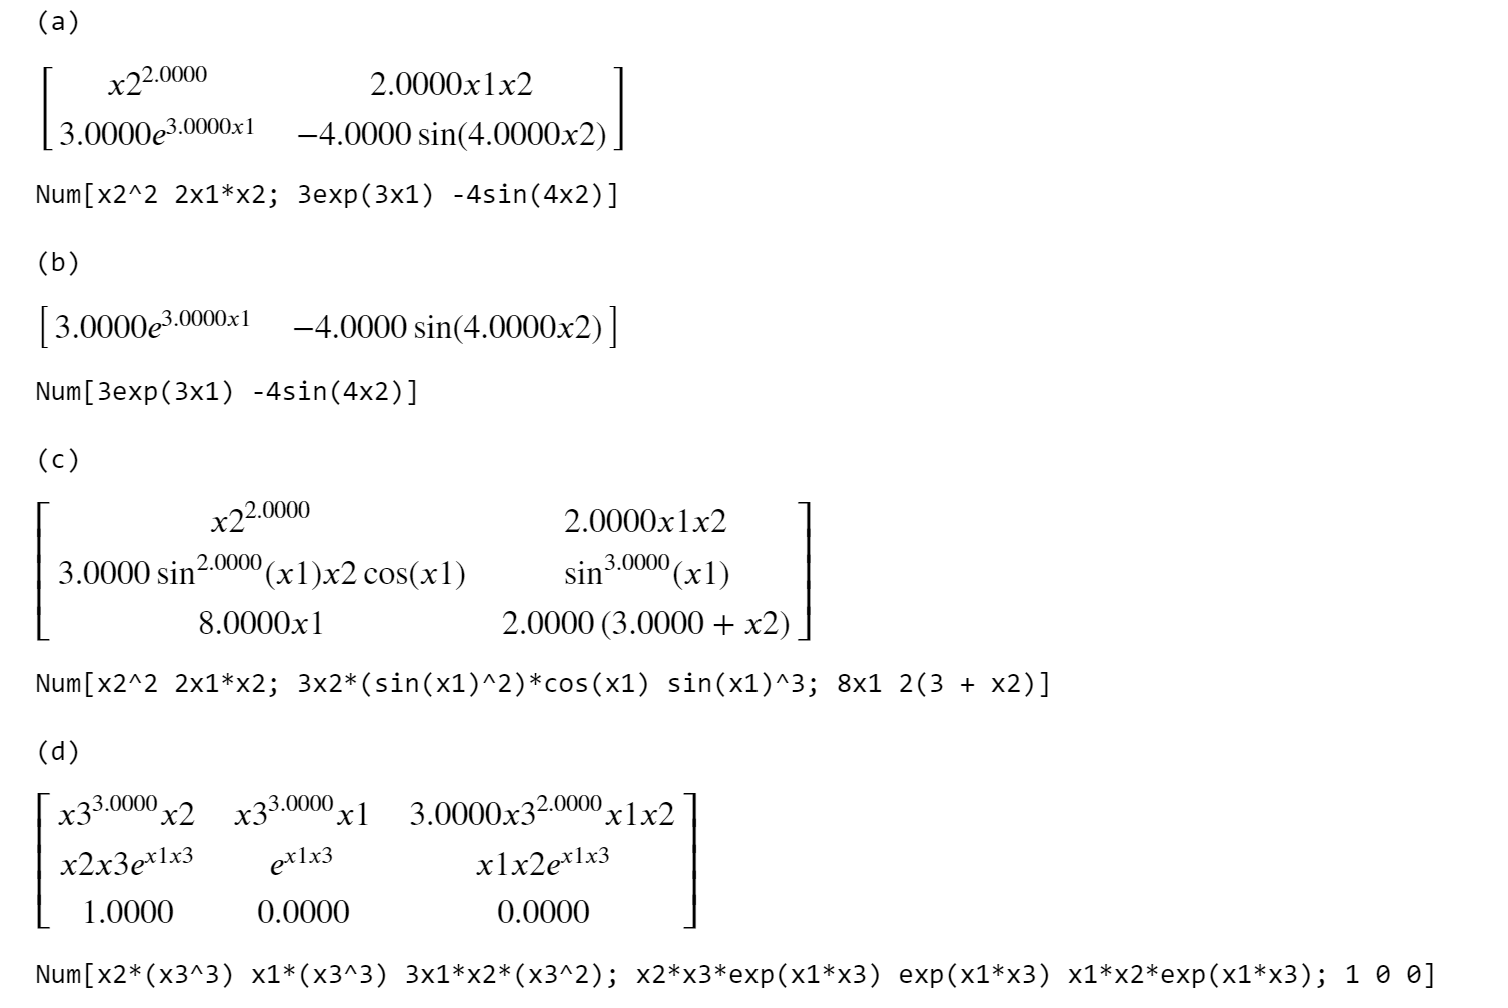
\includegraphics[width=0.95\columnwidth]{graphics/Chap05/ScreenshotJacobianOutputV02.png}
\end{center}

Next, we evaluate the Jacobians at a point. 

\begin{lstlisting}[language=Julia,style=mystyle]
using ForwardDiff
# Example of converting from Symbolic to Numerical Functions
using Symbolics, ForwardDiff

#a)
x0 = [sqrt(2); pi]
# Build a numerical function from the symbolic expression
fa_num = build_function(fa, [x1, x2])
fa_num = eval(fa_num[1])
# Compute the Jacobian of the new function at the test point
Jaca = ForwardDiff.jacobian(fa_num, x0)
println("(a) ")
display(Jaca)
println(" ")

#b) 
x0 = [0.77; 11.6]
fb_num = build_function(fb, [x1, x2])
fb_num = eval(fb_num[1])
# Compute the Jacobian of the new function at the test point
Jacb = ForwardDiff.jacobian(fb_num, x0)
println("(b) ")
display(Jacb)
println(" ")

#c)
x0 = [sqrt(7); 1.0]
fc_num = build_function(fc, [x1, x2])
fc_num = eval(fc_num[1])
# Compute the Jacobian of the new function at the test point
Jacc = ForwardDiff.jacobian(fc_num, x0)
println("(c) ")
display(Jacc)
println(" ")

#d)
x0 = [0.0; 0; 0]
# Build a numerical function from the symbolic expression
fd_num = build_function(fd, [x1, x2, x3])
fd_num = eval(fd_num[1])
# Compute the Jacobian of the new function at the test point
Jacd = ForwardDiff.jacobian(fd_num, x0)
println("(d) ")
display(Jacd)
println(" ")
\end{lstlisting}
\textbf{Output} 
\begin{verbatim}
(a) 
2×2 Matrix{Float64}:
   9.8696  8.88577
 208.774   1.95943e-15
 
(b) 
1×2 Matrix{Float64}:
 30.2233  -2.64922
 
(c) 
3×2 Matrix{Float64}:
  1.0       5.2915
 -0.597294  0.107695
 21.166     8.0
 
(d) 
3×3 Matrix{Float64}:
 0.0  0.0  0.0
 0.0  1.0  0.0
 1.0  0.0  0.0
\end{verbatim}

\vspace*{.2cm}

{\bf In each case, the first-order linear approximation is $\bm{f(x_0) + \frac{\partial f(x_0)}{\partial x} \cdot (x - x_0)}$. All of the Jacobians have been evaluated. }

\section*{Converting Symbolic Functions to Numerical Functions in Julia}

The various Julia packages for computing derivatives do not yet play so nicely with one another. They will someday. The following method was found by applying numerous prompts to ChatGPT4 and Bard (25 Sept 2023). After many false starts, it's actually pretty clean and is what we used above. In the following, the code is explained.

\begin{lstlisting}[language=Julia,style=mystyle]
# Example of converting from Symbolic to Numerical Functions
using Symbolics, ForwardDiff

@variables x1 x2 x3
fd = [x1*x2*(x3)^3; x2*exp(x1*x3); x1]

# Build a numerical function from the symbolic expression
fd_num = build_function(fd, [x1, x2, x3])
fd_num = eval(fd_num[1])

# Test the new function
x0 = [1.0, 2.0, 3.0]
result = fd_num(x0)
println("Result of fd_num(x0): ", result)

# Compute the Jacobian of the new function at the test point
Jac = ForwardDiff.jacobian(fd_num, x0)
println("Jacobian: ", Jac)
\end{lstlisting}

The above code snippet demonstrates how to convert a symbolic function to a numerical function in Julia using the Symbolics and ForwardDiff packages. The symbolic function is defined with variables \(x_1, x_2, x_3\) and consists of three components. The numerical function is then tested at a point \(x_0 = [1.0, 2.0, 3.0]\), and its Jacobian is computed at this point.

\textbf{Importing Packages}
\begin{lstlisting}[language=Julia]
using Symbolics, ForwardDiff
\end{lstlisting}
The Symbolics package is used for symbolic computations, and ForwardDiff is used for automatic differentiation.

\textbf{Defining Symbolic Variables and Function}
\begin{lstlisting}[language=Julia]
@variables x1 x2 x3
fd = [x1*x2*(x3)^3; x2*exp(x1*x3); x1]
\end{lstlisting}
Symbolic variables \(x_1, x_2, x_3\) are defined, and a symbolic function \( \text{fd} \) is created as a vector of three components.

\textbf{Building the Numerical Function}
\begin{lstlisting}[language=Julia]
fd_num = build_function(fd, [x1, x2, x3])
fd_num = eval(fd_num[1])
\end{lstlisting}
The \texttt{build\_function} method from the Symbolics package is used to convert the symbolic function into a numerical function. The \texttt{eval} function is then used to make it callable.

\textbf{Testing the Numerical Function}
\begin{lstlisting}[language=Julia]
x0 = [1.0, 2.0, 3.0]
result = fd_num(x0)
println("Result of fd_num(x0): ", result)
\end{lstlisting}
The numerical function is tested at a point \( x_0 = [1.0, 2.0, 3.0] \).

\textbf{Computing the Jacobian}
\begin{lstlisting}[language=Julia]
Jac = ForwardDiff.jacobian(fd_num, x0)
println("Jacobian: ", Jac)
\end{lstlisting}
The Jacobian of the numerical function at the point \( x_0 \) is computed using ForwardDiff's \texttt{jacobian} function.
\textbf{Output} 
\begin{verbatim}
Result of fd_num(x0): [54.0, 40.171073846375336, 1.0]
Jacobian: [54.0 27.0 54.0; 120.51322153912601 20.085536923187668 40.171073846375336; 
1.0 0.0 0.0]
\end{verbatim}

\begin{center}
\setlength{\fboxrule}{2pt}  % Setting the thickness of the border line
   \fbox{\parbox{0.9\linewidth}{\textcolor{blue}{\bf \large You may prefer the following alternative method.} {\bf It is simpler but has some manual intervention. The purest among you will not like that. Those who just want to get their HW completed, however, may love it!} 
}
} 
\end{center}


\begin{lstlisting}[language=Julia,style=mystyle]
# Exercise in textbook
using Symbolics
# define variables 
@variables x[1:3]

fa = [x[1] * (x[2])^2; exp(3*x[1]) + cos(4*x[2])]
fb = [exp(3*x[1]) + cos(4*x[2])]
fc = [x[1] * (x[2])^2; x[2]*( sin(x[1]) )^3 + 11; 4*(x[1])^2 + ( x[2] +3 )^2]
fd = [x[1]*x[2]*(x[3])^3; x[2]*exp(x[1]*x[3]); x[1]]

# Compute Symbolic Jacobians
#a)
Ja = Symbolics.jacobian(fa, x[1:2])
println("(a) ")
display(Ja)
println(Ja)
println(" ")

#b)

Jb = Symbolics.jacobian(fb, x[1:2]) # The Jacobian function want a vector
                                 # hence, the brackets
println("(b) ")
display(Jb)
println(Jb)
println(" ")

#c)
Jc = Symbolics.jacobian(fc, x[1:2])
println("(c) ")
display(Jc)
println(Jc)
println(" ")

#d)
Jd = Symbolics.jacobian(fd, x)
println("(d) ")
display(Jd)
println(Jd)
println(" ")
\end{lstlisting}
\textbf{Output} 
\begin{center}
    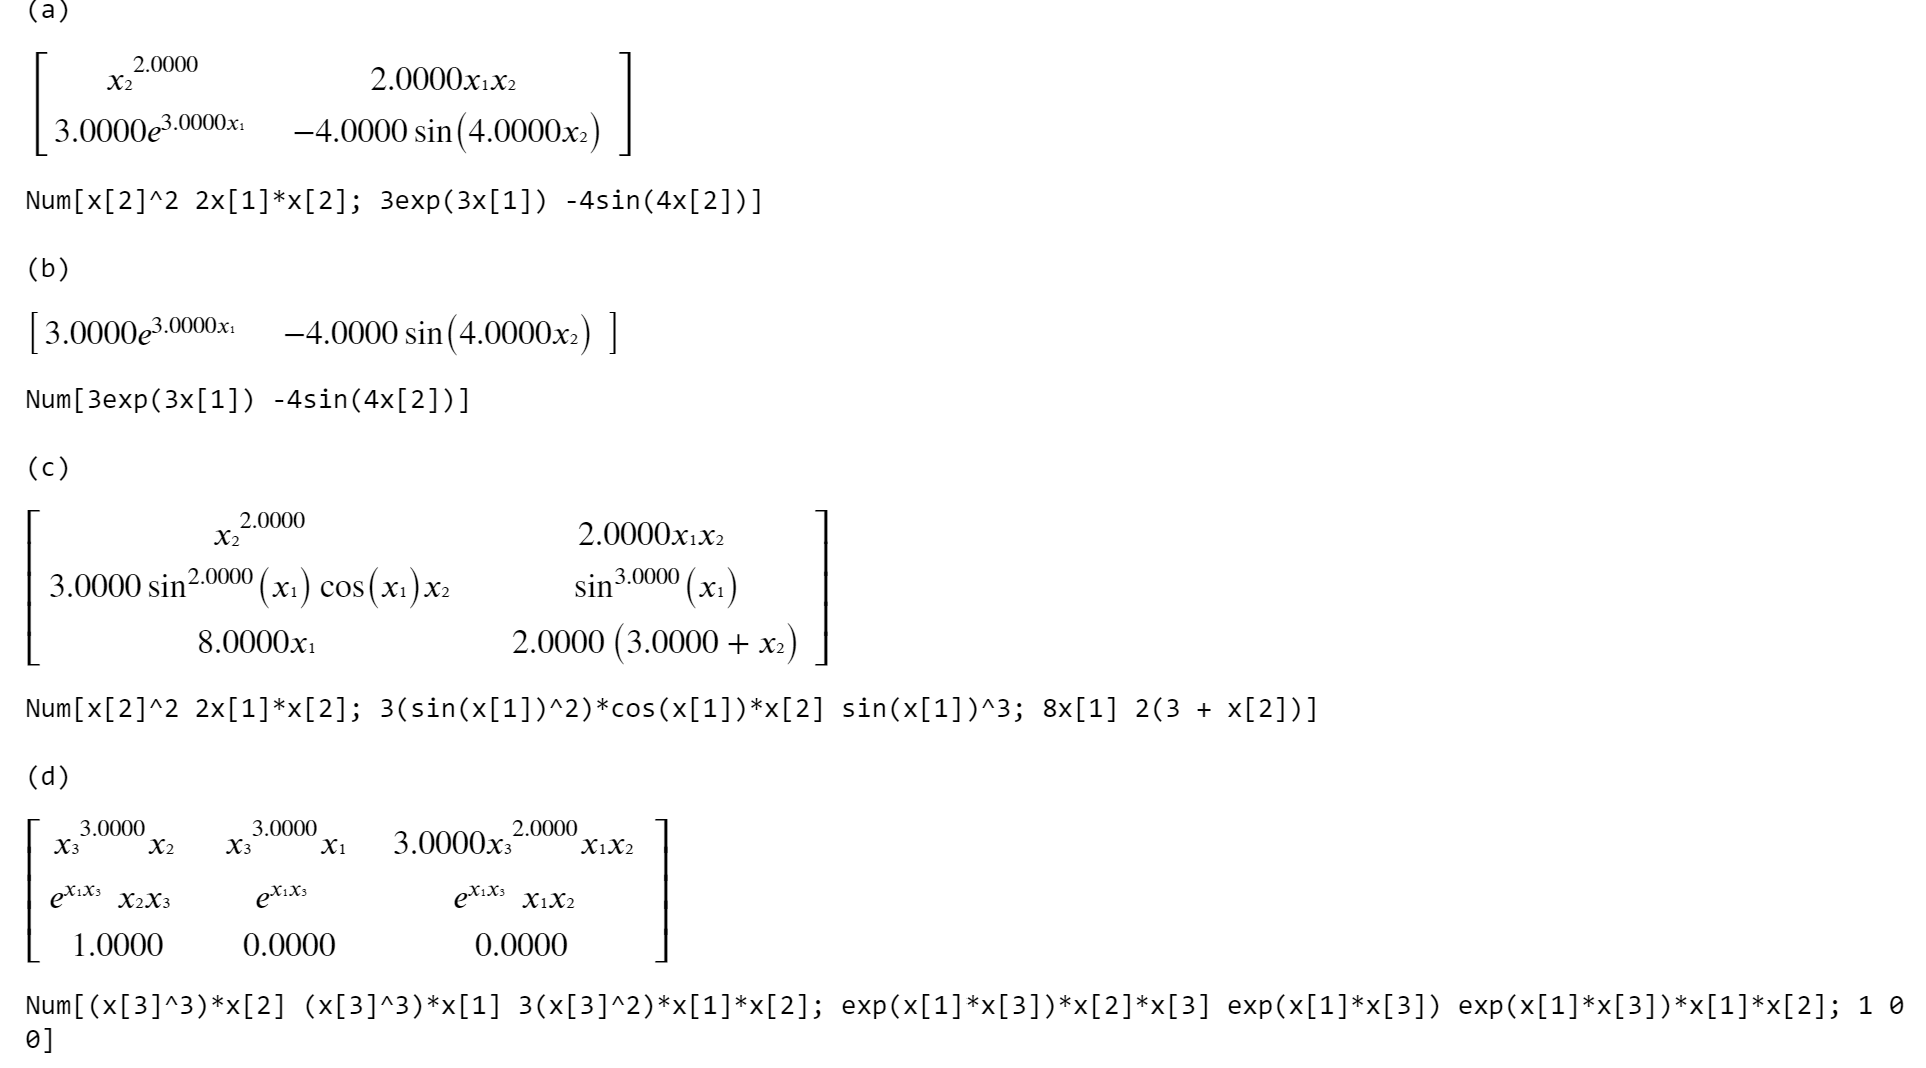
\includegraphics[width=0.95\columnwidth]{graphics/Chap05/ScreenshotJacobianOutputV01.png}
\end{center}

\begin{lstlisting}[language=Julia,style=mystyle]
using ForwardDiff

# Copy and paste to create regular Julia functions. The names are slightly altered so as 
# not to have a conflict with the Symbolic functions fa, fb, fc, fd

fA(x) = [x[1] * (x[2])^2; exp(3*x[1]) + cos(4*x[2])]
fB(x) = [exp(3*x[1]) + cos(4*x[2])]
fC(x) = [x[1] * (x[2])^2; x[2]*( sin(x[1]) )^3 + 11; 4*(x[1])^2 + ( x[2] +3 )^2]
fD(x) = [x[1]*x[2]*(x[3])^3; x[2]*exp(x[1]*x[3]); x[1]];

#a)
x0 = [sqrt(2); pi]
Ja = ForwardDiff.jacobian(fA, x0)
println("(a) ")
display(Ja)
println(" ")

#b)  
x0 = [0.77; 11.6]
Jb = ForwardDiff.jacobian(fB, x0)
println("(b) ")
display(Jb)
println(" ")

#c)
x0 = [sqrt(7); 1.0]
Jc = ForwardDiff.jacobian(fC, x0)
println("(c) ")
display(Jc)
println(" ")

#d)
x0 = [0.0; 0; 0]
Jd = ForwardDiff.jacobian(fD, x0)
println("(d) ")
display(Jd)
println(" ")
\end{lstlisting}
\textbf{Output} 
\begin{verbatim}
(a) 
2×2 Matrix{Float64}:
   9.8696  8.88577
 208.774   1.95943e-15
 
(b) 
1×2 Matrix{Float64}:
 30.2233  -2.64922
 
(c) 
3×2 Matrix{Float64}:
  1.0       5.2915
 -0.597294  0.107695
 21.166     8.0
 
(d) 
3×3 Matrix{Float64}:
 0.0  0.0  0.0
 0.0  1.0  0.0
 1.0  0.0  0.0
\end{verbatim}

\vspace*{.2cm}

One more example, just for fun.

\begin{lstlisting}[language=Julia,style=mystyle]
@variables t x y z a b

# Define a gnarly function with variables t, x, y, z, a, b and 3 components
f_gnarly = [
    sin(a*x^3) + cos(b*exp(y)) + t*z^2 + exp(a - b),
    a*x^2*y - b*t*z + log(x + y + z + 1),
    a*b*t*x*y*z + sin(t) + cos(a) + (atan(exp(b))+11)^z]

# Compute the Jacobian symbolically
Jacobian_gnarly = Symbolics.jacobian(f_gnarly, [t, x, y, z, a, b])

@show f_gnarly
Jacobian_gnarly
\end{lstlisting}
\textbf{Output} 
To save space, we replace $f_{\rm gnarly}(t, x, y, z, a, b)$ with $f(...)$, and note that
$$ {\rm Jac} f(...) = \left[ \begin{array}{cccccc}
\frac{\partial f(...)}{ \partial t} & \frac{\partial f(...)}{ \partial x} & \frac{\partial f(...)}{ \partial y} & 
\frac{\partial f(...)}{ \partial z} & \frac{\partial f(...)}{ \partial a} & \frac{\partial f(...)}{ \partial b}
\end{array}
\right],$$
where

$$ \frac{\partial f(...)}{ \partial t}  =  \left[
\begin{array}{c}
z^{2} \\
 - b z \\
a b x y z + \cos\left( t \right)  \\
\end{array}
\right], 
%
\frac{\partial f(...)}{ \partial x}  =  \left[
\begin{array}{c}
3 x^{2} a \cos\left( x^{3} a \right) \\
\frac{1}{1 + x + y + z} + 2 a x y \\
a b t y z \\
\end{array}
\right],
%
\frac{\partial f(...)}{ \partial y}  = \left[
\begin{array}{c}
 - b e^{y} \sin\left( b e^{y} \right) \\
x^{2} a + \frac{1}{1 + x + y + z} \\
a b t x z \\
\end{array}
\right]
$$
\vspace*{.1cm}
$$
\frac{\partial f(...)}{ \partial z}  =\left[
\begin{array}{c}
2 t z \\
\frac{1}{1 + x + y + z} - b t \\
\left( 11 + \arctan\left( e^{b} \right) \right)^{z} \log\left( 11 + \arctan\left( e^{b} \right) \right) + a b t x y \\
\end{array}
\right]
$$
\vspace*{.2cm}
%
$$
\frac{\partial f(...)}{ \partial a} = \left[
\begin{array}{c}
x^{3} \cos\left( x^{3} a \right) + e^{a - b} \\
x^{2} y \\
 - \sin\left( a \right) + b t x y z \\
\end{array}
\right],  
%
\frac{\partial f(...)}{ \partial b} = \left[
\begin{array}{c}
 - e^{a - b} - e^{y} \sin\left( b e^{y} \right) \\
 - t z \\
\frac{\left( 11 + \arctan\left( e^{b} \right) \right)^{-1 + z} z e^{b}}{1 + \left( e^{b} \right)^{2}} + a t x y z \\
\end{array}
\right].
$$
That would be hard to do by hand. 
\Qed


 
 \subsection{The Gradient}
 
 The \textbf{gradient} is the special name given to the \textbf{transpose of the Jacobian} of a function $f:\real^{n} \to \real$, (i.e., for each $x \in \real^{n}$, $f(x)\in \real$ is a scalar). In Chapter~\ref{sec:MinNoConstraints}, where we deal with optimization, we will show that the gradient of a function  $f:\real^{n} \to \real$ \textbf{points in the direction of maximum increase of the function}, and hence the negative of the gradient points in the \textbf{direction of maximum decrease}. All of the marvelous AI tools at our disposal today rely on the gradient for \textit{training} the neural networks on which the tools are based. \textcolor{blue}{\bf That makes the gradient one of the most important objects in all of Calculus}...and yet, it is just a collection of partial derivatives stacked into a column vector. Who could have imagined that? \\
 
 \begin{tcolorbox}[colback=mylightblue, title=\textbf{The Gradient}, breakable]

 \begin{definition} 
\label{def:Gradient}
The \textbf{gradient} of $f:\real^{n} \to \real$ is the partial derivatives of $f$ with respect to $x_i$ arranged to form a \textbf{column vector}\footnote{In ROB 101 \textit{Computational Linear Algebra}, we did not assume Calculus. When we introduced the gradient, for simplicity, we left it as a row vector.}, instead of a row vector,
\begin{equation}
    \label{eq:GradientDef}
    \nabla f(x_0):=\left[\begin{array}{c}
        \frac{\partial f(x_0)}{\partial x_1} \\  \frac{\partial f(x_0)}{\partial x_2} \\ \vdots \\ \frac{\partial f(x_0)}{\partial x_n} 
    \end{array} \right].
\end{equation} 
The cool symbol $\nabla$ is usually pronounced as ``\textbf{grad}'' and one says ``\textbf{grad f}'' when speaking of $\nabla f$. 
\end{definition}

\begin{rem}
\label{rem:GradAndLinearization}
The Jacobian of $f:\real^{n} \to \real$ is the row vector, 
$\frac{\partial f(x)}{\partial x} := \left[\begin{array}{cccc}
      \frac{\partial f(x)}{\partial x_1} & \frac{\partial f(x)}{\partial x_2} & \cdots & \frac{\partial f(x)}{\partial x_n}
    \end{array} \right] $. It is a $1 \times n$ row vector because each entry, $\frac{\partial f(x)}{\partial x_i}$, is $1 \times 1$ due to $f$ having codomain $\real$, and it has $n$ columns because $x \in \real^{n}$.\\

The gradient is the transpose of the Jacobian. Hence the linearization of $f:\real^{n} \to \real$ can be written as
\begin{equation}
    \label{eq:GradLinearization}
    \begin{aligned}
           f(x) &\approx f(x_0) + \left(\nabla f(x_0) \right)^\top \cdot (x - x_0) \\
           & \approx f(x_0) + \nabla f(x_0) \bullet (x - x_0),
    \end{aligned}
\end{equation}
where $\nabla f(x_0) \bullet (x - x_0)$ is the dot product of the $n \times 1$ gradient vector with the $n \times 1$ vector $(x-x_0)$.  
\end{rem}
\end{tcolorbox}
    


 % \nabla f(x_0):=\left[\begin{array}{c}
 %        \frac{\partial f(x_0)}{\partial x_1} \\  \frac{\partial f(x_0)}{\partial x_2} \\ \vdots \\ \frac{\partial f(x_0)}{\partial x_n} 
 %    \end{array} \right]

\vspace*{.2cm}

\begin{example} 
\label{ex:GradientPartialDerivative} 
Compute the gradient of $f:\real^2 \to \real$, for $f(x_1, x_2) = x_1 \cos(x_2)$ and $x_0=[2~~\pi/4]^\top$.
\end{example}

\textbf{Solution:} We'll compute $\nabla f(x)$ first by hand and then compute both $\nabla f(x)$ and $\nabla f(x_0)$ in software. 

\begin{lstlisting}[language=Julia,style=mystyle]
using Symbolics

@variables x[1:2]
f = x[1] * cos(x[2])
grad_f = Symbolics.gradient(f, [x[1], x[2]])

@show f
@show grad_f

x0 = [2; pi/4]
f_num = build_function(f , x)
f_num = eval(f_num)
# Compute the Jacobian of the new function at the test point
Grad_f_num= ForwardDiff.gradient(f_num, x0)
println(" ")
display(Grad_f_num)
println(" ")

\end{lstlisting}
\textbf{Output} 
$$ \frac{\partial}{\partial x}\left(x_1 \cos(x_2) \right)= \left[\begin{array}{c}
        \frac{\partial }{\partial x_1} \left(x_1 \cos(x_2) \right)\\  \frac{\partial }{\partial x_2} \left(x_1 \cos(x_2) \right)
    \end{array} \right] = \left[\begin{array}{c}
       \cos(x_2)\\  -x_1 \sin(x_2) 
    \end{array} \right].$$


$$ \left. \frac{\partial}{\partial x}\left(x_1 \cos(x_2) \right) \right|_{x_0}=
\left[
\begin{array}{r}
0.70710678 \\
-1.41421356 \\
\end{array}
\right]
$$
\Qed

\vspace*{0.2cm}

One could easily do a ``gnarly'' example with the gradient as well. We leave that to you!

\subsection{A Handy Product Rule for the Gradient and the Jacobian}

On one hand, because partial derivatives are ordinary derivatives taken one variable at a time while holding the others constant, all of the rules for differentiation presented in Chapter~\ref{sec:DiffRules} apply to individual partial derivatives, $\frac{\partial }{\partial x_i}$. On the other hand, applying these rules in a matrix-vector form typically requires tensor notation, which we do not want to touch in this textbook. You are likely very happy about that! There is, however, one useful case where things work out nicely, and we treat that here.


\begin{propColor}{Gradient and Jacobian Meet the Dot Product}{aVectorProductRule}
    Suppose $f:\real^{n} \to \real^{m}$ and $g:\real^{n} \to \real^{m}$ are vector-valued functions and define $h:\real^{n} \to \real$ by 
    \begin{equation}
        h(x):= \left(f(x)\right) ^\top \cdot g(x) = f(x) \bullet g(x), 
    \end{equation}
the dot product of $f$ and $g$. If $f$ and $g$ are both differentiable, then so is $h$ and 
   \begin{equation}
   J_h(x) := \left[ \begin{array}{cccc} \frac{\partial h(x)}{\partial x_1}  & \frac{\partial h(x)}{\partial x_2} & \cdots & \frac{\partial h(x)}{\partial x_n} \end{array} \right] = \left[g(x)\right]^\top \cdot\frac{\partial f(x)}{\partial x}  + \left[f(x)\right]^\top \cdot\frac{\partial g(x)}{\partial x} \end{equation}
and because the gradient is the transpose of the Jacobian, and the transpose of a product equals the product of the transposes in reverse order, we have 
   \begin{equation}
  \nabla h(x) :=  \left[ \begin{array}{c} \frac{\partial h(x)}{\partial x_1}  \\ \frac{\partial h(x)}{\partial x_2}  \\ \vdots  \\  \frac{\partial h(x)}{\partial x_n} \end{array} \right] = \left[ \frac{\partial g(x)}{\partial x} \right]^\top \cdot  f(x)  + 
   \left[ \frac{\partial f(x)}{\partial x} \right]^\top \cdot g(x).
\end{equation}
\end{propColor}

\textbf{Proof:}
The function $h(x)$ is equal to
$$h(x) = \sum_{j=1}^{n} f_j(x) g_j(x). $$ 
Taking the partial derivative of \( h \) with respect to a specific component \( x_i \), we can apply the product rule for single-variable derivatives to obtain,
\begin{align*}
    \frac{\partial h(x)}{\partial x_i} &= \sum_{j=1}^{m} \left( \frac{\partial f_j(x)}{\partial x_i} g_j(x) + f_j(x) \frac{\partial g_j(x)}{\partial x_i} \right) ~~(\text{next, rewrite each sum as a row vector times a column vector}) \\[1em]
    %%
    & = \left[ \begin{array}{cccc} g_1(x)  & g_2(x) & \cdots &g_m(x)  \end{array} \right] \cdot \left[ \begin{array}{c} \frac{\partial f_1(x)}{\partial x_i}  \\ \frac{\partial f_2(x)}{\partial x_i}   \\ \vdots \\ \frac{\partial f_m(x)}{\partial x_i} \end{array} \right]  + 
     \left[ \begin{array}{cccc} f_1(x) & f_2(x) & \cdots & f_m(x)  \end{array} \right] \cdot  \left[ \begin{array}{c} \frac{\partial g_1(x)}{\partial x_i}  \\ \frac{\partial g_2(x)}{\partial x_i}  \\ \vdots  \\  \frac{\partial g_m(x)}{\partial x_i} \end{array} \right] \\[1em]
     %%
     & = \left[g(x) \right]^\top \cdot \left[ \frac{\partial f(x)}{\partial x}   \right]_i  + \left[f(x)\right]^\top \cdot \left[ \frac{\partial g(x)}{\partial x}   \right]_i ,
\end{align*}
 where $\left[ \frac{\partial f(x)}{\partial x}   \right]_i $  and $\left[ \frac{\partial g(x)}{\partial x}   \right]_i$ denote the \(i\)-th columns of the Jacobian matrices. Hence, putting it all together,
$$
J_h(x) := \left[ \begin{array}{cccc} \frac{\partial h(x)}{\partial x_1}  & \frac{\partial h(x)}{\partial x_2} & \cdots & \frac{\partial h(x)}{\partial x_n} \end{array} \right] = \left[g(x)\right]^\top \cdot\frac{\partial f(x)}{\partial x}  + \left[f(x)\right]^\top \cdot\frac{\partial g(x)}{\partial x}.
$$

\Qed



\subsection{(Optional Read:) The Hessian}

Assume that the gradient of the scalar-valued function $f:\real^{n} \to \real$ exists. Then $\nabla f: \real^{n} \to \real^{n}$ is an ($n \times 1)$ vector-valued function. If its partial derivatives with respect to $x=(x_1, x_2, \ldots, x_n)$ exist, then we can compute its Jacobian, which will be an $n \times n$ matrix. The name \href{https://en.wikipedia.org/wiki/Hessian_matrix}{Hessian} for this object is in honor of its inventor, Ludwig Otto Hesse.

\begin{tcolorbox}[colback=mylightblue, title = {\bf Hessian of a Function}, breakable]

\begin{definition} 
\label{def:DefHessian}
The \textbf{Hessian} of $f:\real^{n} \to \real$ is
\begin{equation}
    \label{eq:DefHessian}
   H_f(x):= \frac{\partial \nabla f(x)}{\partial x} := \frac{\partial}{\partial x}\left(  \nabla f(x)\right) =  \left[\begin{array}{cccc}
      \frac{\partial \nabla f(x)}{\partial x_1} & \frac{\partial \nabla  f(x)}{\partial x_2} & \cdots & \frac{\partial \nabla f(x)}{\partial x_n}
    \end{array} \right],
\end{equation}
assuming the indicated partial derivatives exist. 
The Hessian of a function is formed by packaging the column vectors $\frac{\partial \nabla f(x)}{\partial x_j}$ into a matrix. We need to keep in mind that, for each value of $x\in \real^{n}$, the compact and awesome-looking object
$$ H_f(x):= \frac{\partial \nabla f(x)}{\partial x} $$
is really an $n \times n$ matrix: because there are $n$ columns of the form $ \frac{\partial \nabla f(x)}{\partial x_j}$, and each column is an $n$-vector. \textbf{There are software tools that compute the Hessian in one fell swoop. You do not need to first compute the gradient and then the Jacobian, as in the definition}. 

\end{definition}
\end{tcolorbox}


\vspace*{.2cm}

\begin{funColor}{Point Where Many Calc III Students Throw Up Their Hands and Run!}{runaway}
\begin{enumerate}
\renewcommand{\labelenumi}{(\alph{enumi})}
\setlength{\itemsep}{.2cm}
    \item Yes, we forgot to mention that Jacobians, gradients, and Hessians are typically taught in Calc III, Multivariable Calculus, aka Vector Calculus\footnote{Math 215 Multiv \& Vector Calc, at Michigan. In addition to differentiation, it covers multivariable integration as well.}. Because we introduced all of these topics in ROB 101 \textit{Computational Linear Algebra} in the context of root finding for vector-valued functions (Newton-Raphson Algorithm) and minimization of a scalar-valued function depending on $m$-variables (Gradient Descent), we knew you could handle it.
    \item The Julia commands for the Hessian are \texttt{Symbolics.hessian(f, x)} and \texttt{ForwardDiff.hessian(f, x0)}, one line of code. 
    %We'll illustrate these commands in the applications of the Hessian to second-order optimization. 
    \item Below, we write out the Hessian explicitly. It's a mess! Just the thought of having to compute it by hand is terrifying. In math courses, the teachers often take pity on the students and only assign trivial examples for computing the Hessian or have students compute just a few of the terms in the matrix. Consequently, the whole exercise seems pointless to the students. Whence, this textbook.
    \item \textbf{A math fact on \href{https://en.wikipedia.org/wiki/Symmetry_of_second_derivatives}{mixed partial derivatives}}. If 
    $$ \frac{\partial^2 f(x)}{\partial x_i \partial x_j} ~ \text{ and }~ \frac{\partial^2 f(x)}{\partial x_j \partial x_i}$$
    are both continuous functions, then
      $$ \frac{\partial^2 f(x)}{\partial x_i \partial x_j} = \frac{\partial^2 f(x)}{\partial x_j \partial x_i}.$$ \textbf{Hence, for most engineering applications, the Hessian matrix is symmetric.} In math courses, the Hessian is defined to be the transpose of \eqref{eq:DefHessian}. For examples of interest to us, the difference is unimportant because our Hessians are square symmetric matrices.
\end{enumerate}

    
\end{funColor}



 \vspace*{.2cm}

\textbf{Just for the record, we write out $\bm{ H_f(x):= \frac{\partial \nabla f(x)}{\partial x}  }$ as an $\bm{n \times n}$ matrix}. Suppose
$f(x) = f(x_1, x_2, \dots, x_n) $. Then, 
$$\nabla f(x) =\left[
\begin{array}{c}
\frac{\partial f(x)}{\partial x_1} \\[1em]
\frac{\partial f(x)}{\partial x_2}\\[1em]
\vdots \\
\frac{\partial f(x)}{\partial x_n}
\end{array}
\right] .$$
Computing the Jacobian of the gradient, and writing out all of the entries in their $m \times m$ matrix glory, gives
\begin{equation}
    \label{eq:VectorFunctions04}
   H_f(x) =  \frac{\partial \nabla f(x)}{\partial x} := \left[\begin{array}{cccc}
      \frac{\partial \nabla f(x)}{\partial x_1} & \frac{\partial \nabla  f(x)}{\partial x_2} & \cdots & \frac{\partial \nabla f(x)}{\partial x_n}
    \end{array} \right] =\left[\begin{array}{cccc}
      \frac{\partial^2 f(x)}{\partial x_1 \partial x_1} & \frac{\partial^2 f(x)}{\partial x_2 \partial x_1} & \cdots & \frac{\partial^2 f(x)}{\partial x_n \partial x_1} \medskip \\
      \frac{\partial^2 f(x)}{\partial x_1 \partial x_2} & \frac{\partial^2 f(x)}{\partial x_2 \partial x_2} & \cdots & \frac{\partial^2 f(x)}{\partial x_n \partial x_2} \medskip \\
      \vdots & \vdots & \ddots & \vdots \medskip \\
      \frac{\partial^2 f(x)}{\partial x_1 \partial x_n} & \frac{\partial^2 f(x)}{\partial x_2 \partial x_n} & \cdots & \frac{\partial^2 f(x)}{\partial x_n \partial x_n} 
    \end{array} \right].
\end{equation}
In other symbols, the $ij$ component of $H_f(x) :=\frac{\partial \nabla f(x)}{\partial x}$ is
\begin{equation}
\label{eq:HessianEachEntry}
\left[ \frac{\partial \nabla f(x)}{\partial x}  \right]_{ij} = \frac{\partial^2 f(x)}{\partial x_j \partial x_i} ~~\left(= \frac{\partial^2 f(x)}{\partial x_i \partial x_j}  ~~\text{when the partial derivatives are continuous}\right).
\end{equation}

%Examples are given in the next section. 

\subsection{(Optional Read:) More Matrix-Vector Calculus}
\label{sec:MoreMatrixVectorCalculus}

The first thing we want to do is highlight this very useful site: \href{https://www.matrixcalculus.org/}{Matrix Calculus}, an online tool that computes vector and matrix derivatives (matrix calculus), so that you do not have to memorize all the formulas. Now, this site brings up an issue we mentioned previously: there are different conventions for whether $\frac{\partial }{\partial x}$ applied to a scalar-valued function $f:\real^{m} \to \real$ is interpreted as a row vector, which would be a Jacobian, or a column vector, which would be a gradient. Sheesh, you are thinking, after 200 years of Calculus, can't they at least have this settled? Probably not until one of you mounts a worldwide campaign to settle this ``atrocious state of affairs''. We discuss the ``why'' of this below, in case you are interested. Let's note, though, that in spoken and written language, you deal with contradictory meanings and conventions all the time and accept that as part of being fluent. It's no different in math. \textbf{Context usually settles any possible confusion}.


With these comments out of the way, we'll list a few key formulas and derive them so that you have confidence when using matrix-vector calculus.


\begin{propColor}{Key Matrix-vector Calculus Formulas}{MatrixVectorCalculusFormulas}

Most useful formulas for engineers: 
\begin{enumerate}
\renewcommand{\labelenumi}{(\alph{enumi})}
\setlength{\itemsep}{.2cm}
\item For $C$ an $m \times n$ matrix and $x \in \real^{n}$, $\frac{\partial }{\partial x} \left( C  x \right) = C$.

\item For $x \in \real^{n}$, $ \frac{\partial~ }{\partial x} \left(x^\top x\right) = 2 x ^\top $.

\item For $x \in \real^{n}$, $\nabla \left( x^\top x\right) = 2 x$.

\item For $Q$ an $n \times n$ symmetric matrix and $x \in \real^{n}$, $\frac{\partial }{\partial x} \left( x^\top Q x \right)= 2 x^\top \cdot Q $.

\item For $Q$ an $n \times n$ symmetric matrix and $x \in \real^{n}$, $\nabla  \left(x^\top Q  x \right) = 2 Q  x$.

\item For $Q$ an $n \times n$ symmetric matrix and $x \in \real^{m}$, $\frac{\partial \nabla \left(x^\top Q  x \right)}{\partial x}  = 2 Q$ ~~(yes, this is the Hessian of $x^\top Q x$). You will also see it written as 
$\frac{\partial }{\partial x} \left(\frac{\partial \left( x^\top Q x \right)}{\partial x}   \right) = 2 Q$, especially when using the \texttt{Symbolics} package or \texttt{SymPy}.

\end{enumerate}

\textbf{Note:} You will often see a $\frac{1}{2}$ inserted into $ x^\top x$ and $x^\top QX$ so that
$\nabla\left( \frac{1}{2} x^\top x \right) =x$ and $\nabla\left( \frac{1}{2} x^\top Qx \right) =Qx$. There has to be a two or a one-half somewhere! It's your call.
    
\end{propColor}

\vspace*{.2cm}

\textbf{Row vs Column? How to Know:}
The Jacobian matrix provides a linear approximation of a multivariable function. In this context, if \( f: \real^{n} \to \real^{m}\) and $m \ge 2$, then the Jacobian of \( f \) has to be an $m \times n$ matrix. However, when $m =1$, all bets are off! \textbf{Because the gradient is just the transpose of the Jacobian, in many contexts, it seems redundant to use both operations}. The choice to represent either the gradient or Jacobian of $f:\real^{n} \to \real$ as a row vector or a column vector, therefore, depends on conventions, contexts, and the operations you're planning to perform with it. Here's how it usually plays out:

\begin{enumerate}[label=(\roman*)]
    \item When $f:\real^{n} \to \real^{m}$, $m > 1$, then the Jacobian $\frac{\partial f(x)}{\partial x}$ is an $m \times n$ matrix.

    \item When $f:\real^{n} \to \real$, (i.e., $m =1$), then it's 25-75\% whether the Jacobian $\frac{\partial f(x)}{\partial x}$ is a $1 \times n$ row vector (25\%) or $n \times 1$ column vector (75\%), even in this textbook. Whenever possible, we will write the Jacobian as a row vector and use the gradient when we want a column vector. However, we cannot fly in the face of tradition and rewrite famous equations in a form that would be unrecognizable to most users. When treating Lagrange Multipliers in Chapter~\ref{sec:ConstrainedOptimization}, it is very natural to use the gradient for a column of partial derivatives, and we will. When treating Lagrangian Dynamics in Chapter~\ref{sec:LagrangianDynamics}, indicating a column of partial derivatives with a gradient instead of a Jacobian would make the equations unrecognizable, to the point that if you showed them to someone who studied the topic in a different course, they'd think you were from Mars. Alas, sometimes tradition prevails. 

    \item Hence, for us, the Jacobian of $x^\top x$ is a row vector. The extremely useful site, \href{https://www.matrixcalculus.org/}{Matrix Calculus}, the online tool that computes vector and matrix derivatives so that you do not have to, makes the Jacobian of $x^\top x$ a column vector. Outside of this course, when writing out the Jacobian or gradient, always be clear about which convention you're using, especially if your colleagues might be used to a different convention. 

    \item When the gradient of \( f:\real^{n} \to \real\) is represented as a column vector, it is the transpose of the Jacobian matrix of \( f \), 
    $$ \nabla f(x) = \begin{bmatrix}
    \frac{\partial f(x)}{\partial x_1} \\[1em]
    \frac{\partial f(x)}{\partial x_2} \\
    \vdots \\
    \frac{\partial f(x)}{\partial x_n}
    \end{bmatrix} = \left[ J_f(x) \right]^\top.$$
    This is the more common representation, especially in optimization contexts.

    \item The gradient of \( f:\real^{n} \to \real \) can also be represented as a row vector, in which case it's exactly the Jacobian matrix for \( f \),
    $$\nabla f(x) = \begin{bmatrix}
    \frac{\partial f(x)}{\partial x_1} & \frac{\partial f(x)}{\partial x_2} & \dots & \frac{\partial f(x)}{\partial x_n}
    \end{bmatrix} = J_f(x). $$
    We used this convention in ROB 101 \textit{Computational Linear Algebra} to ``keep things simple'' because Calculus was not a prerequisite.
\end{enumerate}
In conclusion, while mathematical conventions can guide the choice of representation, the ultimate decision often depends on the specific context and operations in which the gradient or Jacobian is used. Always prioritize clarity and correctness in your work. \textbf{Always ensure that the dimensionality matches the operations you intend to perform. That's what we mean by context!} \\


\textbf{Proofs of Prop.~\ref{thm:MatrixVectorCalculusFormulas}}

In the following, $x = \left[ \begin{array}{c} x_1 \\x_2 \\ \vdots \\ x_n\end{array} \right]$.\\

\begin{enumerate}
\renewcommand{\labelenumi}{(\alph{enumi})}
\setlength{\itemsep}{.2cm}
\item For $C$ an $m \times n$ matrix and $x \in \real^{n}$, $\frac{\partial }{\partial x} \left( C  x \right) = C$. Express  $C = \left[ \begin{array}{cccc} C_1 & C_2 & \cdots & C_n \end{array} \right]$ in terms of its columns. Then $ C x = x_1 C_1 + x_2 C_2 + \cdots + x_n C_n.$
Hence, 
$\frac{\partial (Cx)}{\partial x_i} = C_i,$
the $i$-th column of $C$. Therefore, 
$ \frac{\partial }{\partial x} \left( C  x \right) = \left[ \begin{array}{cccc} \frac{\partial Cx}{\partial x_1}  & \frac{\partial Cx}{\partial x_2} & \cdots & \frac{\partial Cx}{\partial x_n} \end{array} \right] = C.$\\

Notice what we did: we broke it down to first computing $\frac{\partial }{\partial x_i}$ and then stacked things into rows or columns as required. Keep this in mind when you get stuck making vector computations with derivatives.

\item For $x \in \real^{n}$, $ \frac{\partial~ }{\partial x} \left(x^\top x\right) = 2 x ^\top $.\\

%%%  \frac{\partial }{\partial x_i}

%%% \left[ \begin{array}{cccc}   &    & \cdots &   \end{array} \right]

$x^\top x = x_1^2 + x_2 ^2 + \cdots + x_n^2$. Hence, $\frac{\partial }{\partial x_i}\left( x^\top x\right) = 2 x_i$. Therefore, $\frac{\partial \left( x^\top x\right)}{\partial x} = \left[ \begin{array}{cccc} \frac{\partial \left( x^\top x\right)}{\partial x_1}  & \frac{\partial \left( x^\top x\right)}{\partial x_2} & \cdots & \frac{\partial \left( x^\top x\right)}{\partial x_n} \end{array} \right] = \left[ \begin{array}{cccc}2 x_1  &  2x_2  & \cdots &  2x_n \end{array} \right] = 2 x^\top$.

Alternative proof based on the Product Rule in Prop.~\ref{thm:aVectorProductRule}. We identify $f(x) = x$ and $g(x) = x.$ Hence, $\frac{\partial f(x)}{\partial x} = \frac{\partial g(x)}{\partial x} = \frac{\partial x}{\partial x} =I_n$, where $I_n$ is the $n \times n$ identity matrix. This gives the result immediately.

\item For $x \in \real^{n}$, $\nabla \left( x^\top x\right) = 2 x$.\\

The gradient of a scalar-valued function, being in this textbook, is always the transpose of the Jacobian. The result is immediate from the previous part or from Prop.~\ref{thm:aVectorProductRule}.

\item For $Q$ an $n \times n$ symmetric matrix and $x \in \real^n$, $\frac{\partial }{\partial x} \left( x^\top Q x \right)= 2 x^\top \cdot Q $.\\

This part follows from the next part by taking transposes and noting that that $Q$ symmetric implies that $Q^\top = Q$.

\item For $Q$ an $n \times n$ symmetric matrix and $x \in \real^n$, $\nabla  \left(x^\top Q  x \right) = 2 Q  x$.\\

We apply Prop.~\ref{thm:aVectorProductRule} by identifying $f(x) = x$ and $g(x) =Q  x.$ Hence, $\frac{\partial f(x)}{\partial x} = I_n$, and by part (a) of this problem, $\frac{\partial Q x}{\partial x} = Q$. Hence, 
$$ \nabla \left(x^\top Q  x \right) =  I_n^\top \cdot Q x + Q^\top \cdot x = I_n\cdot Q x + Q^ \cdot x = 2 Q x,$$
because both $I_n$ and $Q$ are symmetric.

\item For $Q$ an $n \times n$ symmetric matrix and $x \in \real^n$, $\frac{\partial \nabla \left(x^\top Q  x \right)}{\partial x}  = 2 Q$ ~~(yes, this is the Hessian of $x^\top Q x^\top$).  \\

Apply part (a) to part (e). 

\end{enumerate}

\section{The Total Derivative or the Chain Rule on Steroids}
\label{sec:TotalDerivative}

Our journey into the realm of differentiation began with the study of functions of a single variable. It was a straightforward world where changes took place in a one-dimensional landscape. But as with most explorations, our innate curiosity led us to broaden our horizons. We ventured into the more intricate domain of functions of several variables, acquainting ourselves with the powerful tool of Jacobians. 

%\jwg{Change to $f:\real^{m} \to \real^{n}$}

Now, imagine combining the simplicity of our initial one-dimensional world with the complexity of the multi-dimensional one. Enter the \textbf{total derivative}. This handy tool allows us to efficiently compute the derivative of a function of a single scalar variable, \( t \), that emerges from the composition of two functions: \( f: \mathbb{R}^{n} \to \mathbb{R}^{m} \) and \( g: \mathbb{R} \to \mathbb{R}^{n} \). In essence, the total derivative marries our initial knowledge with our further explorations, showcasing the true power of differentiation and meriting its place as the last section in this Chapter.

\textbf{Here's the intuition:} Suppose we are given a scalar-valued function of three variables, $f(x, y, z)$, where each of the variables in turn depends on time, denoted as $x(t)$, $y(t)$, and $z(t)$. Then the \textbf{total derivative of $\bm{f}$ with respect to $\bm{t}$ is} 
\begin{equation}
\label{eq:ExampleTotalDerivative}
    \frac{df}{dt} = \frac{ \partial f}{\partial x}  \frac{ d x}{dt}+  \frac{ \partial f}{\partial y} \frac{ d y}{dt} + \frac{ \partial f}{\partial z}  \frac{ d z}{dt},
\end{equation}
which we recognize as being $\bm{\big(}$the rate of change of $f$ with respect to $x$$\bm{\big)}$ \textbf{times} $\bm{\big(}$the rate of change of $x$ with respect to $t$$\bm{\big)}$, plus dot dot dot, \textbf{plus} 
$\bm{\big(}$ the rate of change of $f$ with respect to $z$ $\bm{\big)}$ \textbf{times} $\bm{\big(}$the rate of change of $z$ with respect to $t$$\bm{\big)}$. Hence, \eqref{eq:totalDerivative} is a vector version of the Chain Rule given in Prop.~\ref{thm:DifferentiationRules} Differentiation Rules, parts (d) and (e). Because \eqref{eq:ExampleTotalDerivative} \textcolor{blue}{\bf adds up all of the individual rates of change}, it is given the name \textcolor{blue}{\bf total derivative}.

You may be thinking, ``Couldn't we have simply plugged in $x(t)$, $y(t)$, and $z(t)$ into $f$ and then differentiated with respect to $t$?'' and you would be absolutely correct. It is equivalent, and in some instances, that would be the easier thing to do. But just as it is easier to compute 
$$ \frac{d}{dx}\left(\sin(x^2) \right) =  \left( \cos(x^2) \right)\cdot \left(2x \right) = 2 x \cdot \cos(x^2)$$
with the Chain Rule, than it is to memorize a ginormous table of derivatives that includes the above function, it can be easier to compute the total derivative using a formula such as \eqref{eq:ExampleTotalDerivative}. That is all that is going on here. 



This discussion is formalized in the following definition,which also treats the case of vector valued multivariable functions.


\begin{tcolorbox}[colback=mylightblue, title = {\bf Total Derivative of a Multivariable Function}, breakable]
Suppose that $f:\real^{n} \to \real^{m}$ is a differentiable function and $x:\real \to \real^{n}$ by $x(t) = g(t)$ is also differentiable. 
\begin{definition}
\label{def:totalDerivative}
The \textbf{total derivative} of $f(g(t))$ is $\frac{d}{dt} f(g(t))$, which can be computed as
 \begin{equation}
\label{eq:totalDerivative}
\frac{d}{dt} f(g(t)) = \left. \frac{\partial f(x)}{\partial x}\right|_{x = g(t)} \cdot ~~\frac{d g(t)}{dt} .
\end{equation}



\bigskip

\textbf{Notes:} 
\begin{itemize}
    \item $ \left. \frac{\partial f(x)}{\partial x}\right|_{x = g(t)}$ is the Jacobian of $f(x)$ evaluated 
    at $x=g(t)$.
    \item $\frac{d g(t)}{dt}$ is the ordinary derivative of $g(t)$ with respect to $t$. When $g$ is a vector of functions of $t$, you simply differentiate each of its components.
    \item When $f(x)$ is scalar-valued, that is $f:\real^{n} \to \real$, then expanding out the terms in $\ \frac{\partial f(x)}{\partial x}$ yields a formula like \eqref{eq:ExampleTotalDerivative}.
    \item Indeed, to obtain a formula similar to \eqref{eq:ExampleTotalDerivative} for vector-valued functions, we rewrite \eqref{eq:totalDerivative} as follows:
    \begin{itemize}
        \item let $J_f(x):= \frac{\partial f(x)}{\partial x}$ denote the Jacobian of $f(x)$ and
        \item let $g'(t):=\frac{d g(t)}{dt}$ be the ordinary derivative of $g$ with respect to $t$;
        \item then, the total derivative becomes 
        $$ \frac{d}{dt} f(g(t)) = J_f(g(t)) \cdot g'(t).$$
    \end{itemize}
\end{itemize}

\vspace{.1cm}
\end{definition}
\end{tcolorbox}

\bigskip




\bigskip
We'll illustrate the total derivative on (i) two basic examples to show the mechanics of its computation and (ii) on an example that is much closer to its real use for us: an application to an equation with derivatives, aka, a differential equation. In Chapter~\ref{sec:LagrangianDynamics} we begin laying the groundwork for differential equations through the study of Lagrange's powerful reformulation of Newtonian Mechanics (i.e., F= ma), allowing us to derive dynamical models of multi-link robots and other things that move and go bump in the night.

\bigskip

\begin{example} 
\text{Mechanics of the Total Derivative:} Suppose that $f:\real^2 \to \real$ by
$$f(x_1, x_2) = x_1 \cdot \sin(x_2) $$
and 
$$g(t) =\left[
\begin{array}{c}
g_1(t) \\
g_2(t) \\
\end{array}
\right] = \left[
\begin{array}{c}
t^2\\
t^3
\end{array}
\right]. $$
Compute $\frac{df(t)}{dt} := \frac{d}{dt} f(g(t))$.
\end{example}

\textbf{Solution:} $\frac{df(t)}{dt} = 
2 t \cdot \sin\left( t^{3} \right) + 3 t^{4} \cdot \cos\left( t^{3} \right)$.\\

Using the Chain Rule,
\[
\frac{df(g(t))}{dt} = \left. \frac{\partial f(x)}{\partial x}\right|_{x = g(t)} \cdot  \left[
\begin{array}{c}
\frac{d g_1(t)}{dt} \\
\frac{d g_2(t)}{dt}  \\
\end{array}
\right].
\]
We compute that
\begin{align*}
    \frac{\partial f(x)}{\partial x} &= \left[
\begin{array}{cc}
\sin(x_2) &
x_1 \cos(x_2) 
\end{array}
\right] \\[1em]
\left. \frac{\partial f(x)}{\partial x}\right|_{x = g(t)} &= \left[ \begin{array}{cc}
\sin(t^2) &
t^2 \cdot \cos(t^3) 
\end{array}
\right].
\end{align*}
and
$$
\left[
\begin{array}{c}
\frac{d g_1(t)}{dt} \\
\frac{d g_2(t)}{dt}  \\
\end{array}
\right] = \left[
\begin{array}{c}
2 t\\
3 t^2
\end{array}
\right].
$$

Putting it all together, we obtain
$$
\frac{df(g(t))}{dt} =  \left. \frac{\partial f(x)}{\partial x}\right|_{x = g(t)} \cdot  \left[
\begin{array}{c}
\frac{d g_1(t)}{dt} \\
\frac{d g_2(t)}{dt}  \\
\end{array}
\right] = \left[ \begin{array}{cc}
\sin(t^2) &
t^2 \cdot \cos(t^3) 
\end{array}
\right] \cdot  \left[
\begin{array}{c}
2 t\\
3 t^2
\end{array}
\right] = 2 t \sin\left( t^{3} \right) + 3 t^{4} \cos\left( t^{3} \right).
$$
\Qed

\bigskip

\textbf{You will need to do examples like this by hand in various courses. In code, to check your work, you could do the following:}

\begin{lstlisting}[language=Julia,style=mystyle]
using Symbolics

# Create a custom function to make differentiation convenient
function deriv(f, x)
    return expand_derivatives.(Symbolics.Differential(x)(f))
end

@variables x1, x2, t

f = x1*sin(x2)

# Compute the Jacobian of f with respect to x1, x2
Jac = Symbolics.jacobian([f], [x1, x2])

# Define the functions x1(t), x2(t)
x1_def = t^2
x2_def = t^3


# Compute the derivatives of x1(t) and x2(t) with respect to t
derivatives = [deriv(x1_def, t), deriv(x2_def, t)]

# Compute the total derivative of f using the chain rule (matrix multiplication)
df_dt_chain = Jac * derivatives

# Substitute in for x1(t) and x2(t)
df_dt = substitute(df_dt_chain, Dict(x1 => x1_def, x2 => x2_def))
    
# The result of df_dt_chain = Jac * derivatives is a 1 x 1 column vector. 
# In Julia, we need to extract the first (and only) element of this 
# vector using df_dt_chain[1] to produce a scalar-valued function. Why?
# The simplify command in Symbolics expects a scalar and not a vector.
# You can also use broadcasting to make it work
#    
df_dt = Symbolics.simplify(df_dt[1],expand=true) # extract scalar


println("\nThe total derivative of f with respect to t is:\n\n", df_dt)
\end{lstlisting}
\textbf{Output} 
\begin{verbatim}
The total derivative of f with respect to t is:

2t*sin(t^3) + 3(t^4)*cos(t^3)
\end{verbatim}

\bigskip

\begin{example} \text{Mechanics of the Total Derivative:} Suppose that $f:\real^3 \to \real$ by
$$f(x, y, z) = x^3 + y^3 + z^3$$
and 
$$\left[
\begin{array}{c}
x(t) \\
y(t) \\
z(t)
\end{array}
\right] = \left[
\begin{array}{c}
e^t\\
e^t \sin(t) \\
e^t \cos(t)
\end{array}
\right]. $$
Compute $\frac{df(t)}{dt} := \frac{d}{dt} f(x(t), y(t), z(t))$.
\end{example}

\textbf{Solution:} $\frac{df(t)}{dt} = 3e^{3t} - 3\cos^2(t) \cdot \sin(t) + 3\cos(t)  \cdot \sin^2(t)$.\\

We solve this one using non-vector notation so that you can find a preference: Using the Chain Rule and leaving out the arguments on the functions, we have
\[
\frac{df}{dt} = \frac{\partial f}{\partial x} \frac{dx}{dt} + \frac{\partial f}{\partial y} \frac{dy}{dt} + \frac{\partial f}{\partial z} \frac{dz}{dt}.
\]
We compute that
\[
\frac{\partial f}{\partial x} = 3x^2, \quad \frac{\partial f}{\partial y} = 3y^2, \quad \text{and} \quad \frac{\partial f}{\partial z} = 3z^2,
\]
and
\[
\frac{dx}{dt} = e^t, \quad \frac{dy}{dt} =  e^t \sin(t) + e^t \cos(t) , \quad \text{and} \quad \frac{dz}{dt} =e^t \cos(t) - e^t \sin(t).
\]
Combining these values and doing the required substitutions, we obtain
\begin{align*}
    \frac{df}{dt} &= \underbrace{3\left(e^t \right)^2}_{\frac{\partial f}{\partial x}} \cdot \underbrace{\left(e^t \right)}_{\frac{dx}{dt}} + \underbrace{3\left(e^t\sin(t)\right)^2}_{\frac{\partial f}{\partial y}} \cdot \underbrace{\left(  e^t\sin(t) + e^t\cos(t) \right)}_{\frac{dy}{dt}} + \underbrace{3 \left(e^t\cos(t) \right)^2}_{\frac{\partial f}{\partial z}} \cdot \underbrace{\left( e^t\cos(t) -e^t\sin(t)\right)}_{\frac{dz}{dt}}\\
    & = \textcolor{red}{\text{\bf (lol, where's Julia?)}}\\
    & = 3e^{3t} - 3\cos^2(t) \cdot \sin(t) + 3\cos(t)  \cdot \sin^2(t).
\end{align*}

\emstat{\textbf{Some Perspective:} The above illustrates the ``grind of Calculus''. Everyone dislikes it. You will have to do some messy calculations in your Science and Engineering courses. Once again, this is just part of the learning process, akin to running wind sprints in sports---they're no fun, but they make you better in the game! As a practicing STEM professional, you will use ``productivity tools'', such as Julia or MATLAB. As a student, you can always check your HW with Julia! \textcolor{blue}{\bf On an exam, you are unlikely to face a math calculation like this one because the instructor is evaluating your mastery of some newly acquired STEM skills (we hope) and not your ability to do fussy algebra.}}

\begin{lstlisting}[language=Julia,style=mystyle]
using Symbolics

# Create a custom function to make differentiation convenient
function deriv(f, x)
    return expand_derivatives.(Symbolics.Differential(x)(f))
end

@variables x, y, z, t

f = [x^3 + y^3 + z^3]

# Compute the Jacobian of f with respect to x, y, z
Jac = Symbolics.jacobian(f, [x, y, z])

# Define the functions x(t), y(t), and z(t)
x_def = exp(t)
y_def = sin(t)
z_def = cos(t)

# Compute the derivatives of x(t), y(t), and z(t) with respect to t
derivatives = [deriv(x_def, t), deriv(y_def, t), deriv(z_def, t)]

# Compute the total derivative of f using the chain rule (matrix multiplication)
df_dt_chain = Jac * derivatives

# Substitute in for x(t), y(t), and z(t)
df_dt = substitute(df_dt_chain, Dict(x => x_def, y => y_def, z => z_def))
    
# The result of df_dt_chain = Jac * derivatives is a 1 x 1 column vector. 
# In Julia, we need to extract the first (and only) element of this 
# vector using df_dt_chain[1] to produce a scalar-valued function. Why?
# The simplify command in Symbolics expects a scalar and not a vector.
# You can also use broadcasting to make it work
#    
df_dt = Symbolics.simplify.(df_dt,expand=true) # broadcasting, note the dot

println("\nThe total derivative of f with respect to t using the chain rule is:\n\n", df_dt)

\end{lstlisting}
\textbf{Output} 
\begin{verbatim}
The total derivative of f with respect to t using the chain rule is:

3exp(3t) - 3(cos(t)^2)*sin(t) + 3cos(t)*(sin(t)^2)
\end{verbatim}

\vspace*{.2cm}

\textbf{Setting the stage for the next example:} The following is called a linear system of differential equations, 
\begin{equation}
\label{eq:SpecificLinearODE}
\begin{bmatrix}
\frac{d x_1(t)}{dt} \\
\frac{d x_2(t)}{dt} \
\end{bmatrix}
=
\begin{bmatrix}
0 & 1 \\
-1 & -1
\end{bmatrix}
\begin{bmatrix}
x_1(t) \\
x_2(t)
\end{bmatrix} = \begin{bmatrix}
x_2(t) \\
-x_1(t) - x_2(t)
\end{bmatrix}.
\end{equation}
Physically, this system of equations, with derivatives on the left side and unknown (aka, to be found) functions of time on the right side, represents a linear approximation of a pendulum with friction at the pivot: $x_1(t)$ is the angle of the pendulum and $x_2(t)$ is the angular velocity of the pendulum.

We do not yet know how to find the unknown functions, $x_1(t)$ and $x_2(t)$. When we come to this later in the book, we'll understand that a solution to this system of equations is not so different than what is required for solving any system of equations: we need to find functions that, when substituted into the left side (which involves taking their derivatives), equals the right side (which involves only substituting in the functions). That's why they are called equations: an equality holds. 

The next example asks (and answers) an intriguing question: without knowing the solutions to the above differential equations, can we prove that the solutions do not explode? That is, 
\begin{equation}
\label{eq:LimitForSpecificLinearODE}
    \lim_{t \to \infty} \left(x_1(t) \right)^2 + \left(x_2(t) \right)^2
\end{equation}
is finite? And just maybe, that it even equals zero? Huh? We do not know the solution, but we seek to determine some of its properties anyway? That seems like a power mindset! \textcolor{blue}{\bf To answer these questions, we will use the total derivative.} 

\vspace*{.2cm}

\begin{example} 
\label{ex:TotalDerivativeWithODE}
For the differential equations in \eqref{eq:SpecificLinearODE}: 
\begin{enumerate} 
\renewcommand{\labelenumi}{(\alph{enumi})}
\setlength{\itemsep}{.2cm}
    \item Show that the limit in \eqref{eq:LimitForSpecificLinearODE} does not blow up.
    \item Bonus: Give a plausible argument that the limit is, in fact, equal to zero.
\end{enumerate}
    
\end{example}

\textbf{Solution:} Define a function $V(x_1, x_2):= (x_1)^2 + (x_2)^2$, which is the norm squared of the vector $(x_1, x_2)$. We compute its total derivative with respect to time, $\frac{dV(x_1(t), x_2(t))}{dt},$ using the Chain Rule,
\begin{align*}
    \frac{d}{dt}V(x_1(t), x_2(t)) &= \frac{\partial V(x_1(t), x_2(t))}{\partial x_1 } \cdot \frac{d x_1(t)}{dt} + 
     \frac{\partial V(x_1(t), x_2(t))}{\partial x_2 } \cdot \frac{d x_2(t)}{dt} \\[1em]
     &= \underbrace{2 x_1(t)}_{\frac{\partial V}{\partial x_1 }} \cdot \frac{d x_1(t)}{dt} + 
     \underbrace{2 x_2(t)}_{\frac{\partial V}{\partial x_2}} \cdot \frac{d x_2(t)}{dt} \\[1em]
     & = 2 x_1(t) \cdot \underbrace{x_2(t)}_{\frac{d x_1(t)}{dt}} + 2 x_2(t) \cdot \underbrace{(-x_1(t) - x_2(t) )}_{\frac{d x_2(t)}{dt}} ~~(\text{plugging in from \eqref{eq:SpecificLinearODE}})\\[1em]
     & = -2 (x_2(t))^2.
\end{align*}

Because 
\begin{equation}
    \frac{d}{dt}V(x_1(t), x_2(t)) =  -2 (x_2(t))^2 \le 0
\end{equation}
for all $t$, Prop.~\ref{thm:Monotonicity} implies that the function $V(x_1(t), x_2(t))$ is nonincreasing! We do not know the actual time-function $V(t) = V(x_1(t), x_2(t))$, but we know that its initial value at time $t=0$ is its largest possible value (otherwise, it could not be nonincreasing). Therefore, the limit in \eqref{eq:LimitForSpecificLinearODE}, if it exists, cannot go to infinity. \textbf{That settles the first part of the question, which is already an awesome demonstration of the total derivative in action}. What about the second part of the question? 

\textbf{Bonus: The limit likely goes to zero, and the reasoning is as follows.} If a pendulum is not at rest at the downward position, it oscillates. That's what pendulums are designed to do. Now, as long as the angular velocity $x_2(t)$ of the pendulum is non-zero, the time rate of change of $V(x_1(t), x_2(t))$ is negative, so $V(x_1(t), x_2(t))$ continues to decrease. The angular velocity of the pendulum goes to zero when the pendulum reaches one of its two ``extreme swing angles'' and reverses course. So, as long as the pendulum is not at rest in its downward position, $V(x_1(t), x_2(t))$ is decreasing. It cannot decrease below zero because $(x_1(t))^2 + (x_2(t))^2$ represents the norm squared of the vector $(x_1(t), x_2(t))$. Hence $V(x_1(t), x_2(t))$ likely converges to zero as $t \to \infty$. At Michigan, the course EECS 562: Nonlinear Systems and Control makes this argument fully rigorous. 

\begin{lstlisting}[language=Julia,style=mystyle]
using Symbolics

# Create a custom function to make differentiation convenient
function deriv(f, x)
    return expand_derivatives.(Differential(x)(f))
end

@variables x1 x2
x=[x1 x2]

# Define the differential equations as a vector
dx_dt = [x2; -x1 - x2]

# Define a function V(x)
V = x1^2 + x2^2 

# Compute the Jacobian of V with respect to x
Jac_V = Symbolics.jacobian([V], x)

# Compute the total derivative of V using the chain rule 
dV_dt = Jac_V * dx_dt

# The result of the matrix multiplication Jac_V * dx_dt 
# is a 1 x 1column vector. 
# Since we are interested in the scalar value of the derivative, 
# we extract the first (and only) element of this vector using dV_dt[1].
#
# Simplify the result and expand polynomial expressions
#
dV_dt = Symbolics.simplify(dV_dt[1], expand=true)

println("The total derivative of V with respect to t using the chain rule is:\n \n", dV_dt)

\end{lstlisting}
\textbf{Output} 
\begin{verbatim}
The total derivative of V with respect to t using the chain rule is:
 
-2(x2^2)
\end{verbatim}
\Qed







%% For the end of the section
\textbf{Bottom Line:}

\begin{itemize}
    \item \textbf{Multidimensional Chain Rule:} The total derivative can be thought of as the chain rule's multidimensional counterpart. While the partial derivative captures the rate of change of a multivariable function with respect to a single variable, the total derivative encapsulates the compounded effect of each variable's rate of change on the function. It's the chain rule, but on a grander scale.
    
    \item \textbf{Versatility:} While plugging in \(x(t)\), \(y(t)\), and \(z(t)\) directly into \(f\) and differentiating is a straightforward approach, the total derivative offers a more structured method. This becomes especially valuable when dealing with functions where the relationship between variables isn't immediately clear (such as our differential equation) or when the function's form makes direct differentiation less intuitive.
    
    \item \textbf{Efficiency:} Just as the chain rule can simplify differentiation for certain composite functions, the total derivative can be more efficient for functions of multiple variables. Instead of working out derivatives for every possible combination of functions, the total derivative provides a systematic approach that breaks the computation down into simpler pieces. Recall that Automatic Differentiation, heavily used in Machine Learning, also uses the Chain Rule to decompose a complicated derivative into simpler parts.
\end{itemize}

\vspace*{.2cm} 

\begin{funColor}{Let's ask ChatGPT4}{ChatGPT4ImportantMath}
    
\textcolor{blue}{\bf \large Grizzle to ChatGPT4: What do you think is the most important mathematical tool used for training your neural networks?}\\

\textbf{Answer: The training of neural networks, like mine, relies on a combination of mathematical concepts, algorithms, and techniques. If we had to pinpoint the most fundamental mathematical tool, it would be:}

\begin{enumerate}
    \item \textbf{Calculus and the Chain Rule:} The backpropagation algorithm, which is central to training deep neural networks, is essentially an application of the chain rule from calculus. It computes the \textcolor{blue}{\bf gradient of the loss function with respect to each weight} by propagating the gradient backward through the network.
\end{enumerate}

Other important mathematical tools and concepts include:

\begin{enumerate}
    \setcounter{enumi}{1}
    \item \textbf{Linear Algebra:} Neural networks involve a lot of matrix multiplications and transformations, especially in architectures like convolutional neural networks (CNNs) and recurrent neural networks (RNNs).
    
    \item \textbf{Probability and Statistics:} These are crucial for understanding concepts like regularization, dropout, and batch normalization. They also play a role in the design of loss functions and the interpretation of neural network outputs, especially in classification tasks.
    
    \item \textbf{Optimization:} Gradient descent and its variants (like stochastic gradient descent, Adam, RMSprop, etc.) are optimization algorithms used to adjust the weights of the network to minimize the loss function.
    
    \item \textbf{Differential Equations:} Especially relevant in the context of understanding and designing recurrent neural networks and more recent architectures like Neural ODEs.
    
    \item \textbf{Information Theory:} Concepts like entropy and cross-entropy, which are foundational to certain loss functions (e.g., the cross-entropy loss for classification tasks).
\end{enumerate}

While the chain rule and calculus form the backbone of the training process, the successful training and deployment of neural networks require a holistic understanding and application of various mathematical tools and concepts.\\

\textcolor{blue}{\bf Grizzle: Just like Robotics!}\\

\hfill 13 October 2023, Saint-R\'emy-de-Provence, France

\end{funColor}

\section{(Optional Read): Proofs Associated with the Chapter}

 

\begin{tcolorbox}[title=\textcolor{black}{Proof of Prop.~\ref{thm:DifferntiableImpliesContinuous} (Differentiable at $x_0$ Implies Continuous at $x_0$)}, sharp corners, colback=green!30, colframe=green!80!blue, breakable, fonttitle=\bfseries]

Suppose $f:[a, b] \to \real$ is differentiable at $x_0 \in [a, b]$. Then, $f$ is continuous at $x_0$. 

\end{tcolorbox}

\textbf{Proof:} If we assume $f$ is differentiable at $x_0$, then
$$L:= \lim_{h \to 0} \frac{f(x_0 + h) - f(x_0)}{h} $$
exists and is finite. We can rewrite the above as 
$$\lim_{h \to 0} \left[ \frac{f(x_0 + h) - f(x_0)}{h} - L \right] = 0, $$
or in other symbols, if we define
$$ {\rm err}(h):=  \frac{f(x_0 + h) - f(x_0)}{h} - L $$
to be the error in the limit for $h\neq 0$, then $\displaystyle \lim_{h \to 0} {\rm err}(h) = 0. $ But that, in turn by Prop.~\ref{thm:LimitProdRatio}, implies that 
$\displaystyle \lim_{h \to 0} h \cdot {\rm err}(h) = 0$, which gives us
$$ \lim_{h \to 0} \left[ f(x_0 + h) - f(x_0) - h \cdot L \right] = 0.$$
From this, we deduce that 
$$ \lim_{h \to 0}  f(x_0 + h) = \lim_{h \to 0} \left[ f(x_0) - h \cdot L \right]  =   f(x_0) - \lim_{h \to 0}  h \cdot L  = f(x_0).$$
In other words, $f$ is continuous at $x_0$ by Definition~\ref{def:Continuity}.
\Qed




